\documentclass{beamer}   % {article} [handout]
\usepackage{etoolbox}
%\setbeameroption{show notes}
%\usepackage{beamerarticle}
\usepackage{graphicx}
%\mode<handout>{Differential Equations Notes}


 



\usetheme{Frankfurt}%
\usecolortheme{seagull}
\logo{
\includegraphics[height=.25in]{img/clarksonGreen}}

\definecolor{garnet}{RGB}{136,0,0}
%\definecolor{clarksonGreen}{RGB}{0,71,28}
\definecolor{clarksonGreen}{RGB}{0,52,21}
\setbeamercolor{palette primary}{fg=clarksonGreen,bg=white}
\setbeamercolor{palette secondary}{fg=clarksonGreen,bg=white}
\setbeamercolor{palette tertiary}{fg=clarksonGreen,bg=white}
\setbeamercolor{palette quaternary}{bg=clarksonGreen,fg=white}
\setbeamercolor{block title}{fg=black,bg=black!15}
\setbeamercolor{block body}{fg=black,bg=black!10}
\setbeamercolor{titlelike}{bg=clarksonGreen,fg=white} % parent=palette quaternary}

\newcommand{\half}{\mbox{$\frac{1}{2}$}}
\newcommand{\deltat}{\mbox{$\triangle t$}}
\newcommand{\deltax}{\mbox{$\triangle x$}}
\newcommand{\deltay}{\mbox{$\triangle y$}}

\newcommand{\deriv}[2]{\frac{d}{d#2}#1}
\newcommand{\derivTwo}[2]{\frac{d^2}{d#2^2}#1}

\newcommand{\lp}{\left(}
\newcommand{\rp}{\right)}


\includeonlylecture{Linear-Equations}
\includeonly{week2-Day1}
%test

\newtoggle{clicker}
\toggletrue{clicker}
%\togglefalse{clicker}
\newcounter{clickerQuiz}      % Create a counter to determine which clicker quiz to give
\setcounter{clickerQuiz}{1}   % Set the counter to 1, 2, or 3 for the section number


\begin{document}
\author{Kelly Black and Guangming Yao}
\institute{Clarkson University}


\part{Introduction}
\lecture{Introduction}{Introduction}
\section{Introduction}

\title{Ordinary Differential Equations}
\subtitle{Introduction}
\date{27 Aug 2012}

\begin{frame}
  \titlepage
\end{frame}

\begin{frame}
  \frametitle{Outline}
  \tableofcontents[pausesection,hideothersubsections,sectionstyle=show/hide]
\end{frame}

\subsection{Syllabus}
\begin{frame}
  \frametitle{Syllabus}

  Read the syllabus! The syllabus will take precedence over any
  discrepancies here. It includes \textbf{all} of our policies. We
  will not cover them all here.

  Faculty: \\
  \begin{tabular}{l@{\hspace{3em}}l@{\hspace{3em}}l}
    Kelly Black                      & Guangming Yao    \\
    361B Science Center              & 363 Science Center   \\
    268-3831                         & 268- 6496\\
    kjblack@gmail.com                &  gyao@clarkson.edu\\ [10pt]
  \end{tabular}

\end{frame}


\begin{frame}
  \frametitle{Materials}

  \begin{itemize}
  \item {\em Differential Equations and Linear Algebra}, second
    edition
  \item Recitation manual \\
    The UPS Store, \\
    200 Market St, \\
    315.265.4565, \\
    store5986$@$theupsstore.com
  \item Turning Point Technologies ResponseCard RF LCD clicker \\
    \url{https://store.turningtechnologies.com} \\
    The Clarkson University promotional code is Z0k0.
  \end{itemize}
  
\end{frame}


\begin{frame}
  \frametitle{Test Dates}

   The tests will be given 18 September, 30 October,
  and 29 November. The exams will take place in the evenings from
  7:00pm to 8:20pm. You should bring your own pencils.  The professor
  will not have any spare materials. The location will vary depending
  on your recitation section, and your room assignments will be given
  prior to the exams.
  
\end{frame}


\begin{frame}
  \frametitle{Grading}

   \begin{tabular}[t]{rl}
    45\% & 3 Tests. \\
    20\% & Final Exam. \\
    15\% & Homework and Webwork. \\
    15\% & Quiz. \\
     5\% & Clickers
  \end{tabular}

  \begin{itemize}
  \item The right to miss a scheduled exam and take a make up exam can
    be awarded only by your professor.
  \item If for some reason you must miss an exam, you must apply in
    writing {\bf before} the exam.
  \item In case of emergency contact the professor as soon as possible
    and provide documentation to confirm why you cannot take part in
    the exam. 
  \item An unexcused absence will result in a grade of zero on the
    exam.
  \end{itemize}


  
\end{frame}


\begin{frame}
  \frametitle{Academic Accommodations}

  If you require any kind of special
  accommodation please see your professor.  Requests for academic
  accommodations must be made during the first three weeks of the
  semester, except for unusual circumstances.  Students must register
  with the Office of Accommodative Services, located in the Student
  Success Center, 110 ERC, to verify their eligibility for appropriate
  accommodations.
  
\end{frame}

\begin{frame}
  \frametitle{Clickers}

  We will start using the clickers this Friday. Each day one or more
  questions will be asked.

  You need to register your clicker. Go to our course page on moodle:
  \begin{enumerate}
  \item Choose the ``clicker ID'' option at the top of the page.
  \item Enter your clicker Device ID (found on the back of the
    clicker.)
  \item Click on the submit button.
  \item Click on the ``next'' button.
  \item Click on ``Submit all and finish.''
  \item Confirm your choice.
  \item Click on ``Finish Review'' at the bottom of the page.
  \end{enumerate}

  If you do not click on ``Finish Review'' your device ID may not be saved.
   
  
\end{frame}


\begin{frame}
  \frametitle{Recitations}

  \begin{itemize}
  \item Take place every Thursday.
  \item Will have a quiz almost every session.
  \item Some days the quiz will consist of the pre-class activity in
    your lab manual. (Random!)
  \item The recitation is where you \textbf{DO} things. It is where
    you will learn the most in this class.
  \end{itemize}
\end{frame}

\subsection{What is a Differential Equation}


\begin{frame}
  \frametitle{What is a DE?}

  Given
  \begin{eqnarray*}
    y'(x) & = & y(x),
  \end{eqnarray*}
  what is $y(x)=?$

  \begin{eqnarray*}
    \deriv{y(x)}{x} & = & y(x)
  \end{eqnarray*}

\end{frame}


\begin{frame}{Question:}
  Given
  \begin{eqnarray*}
    y'' + 3y' +2y & = & 0
  \end{eqnarray*}

  what is $y(x)$?

  \uncover<2->{
    Note: we leave often leave off the function notation.
    }

  \uncover<3->{
    Why? We are lazy!
    }

\end{frame}

\begin{frame}
  \frametitle{Notation}
  \begin{eqnarray*}
    \dot{y} & = & \deriv{y}{t} \\
    \only<2->{\ddot{y} & = & \derivTwo{y}{t} }\\
    \only<3->{y' & = & \mathrm{depends.... usually ~~} \deriv{y(x)}{x} }\\
    \only<4->{y'' & = & \derivTwo{y(x)}{x} }
  \end{eqnarray*}
\end{frame}

\begin{frame}
  \frametitle{Nomenclature}
  
  \vfill

  $\deriv{y}{x}$ - then ``ordinary differential equation.''

  \vfill

  $\frac{\partial y}{\partial x}$ - then ``partial differential
  equation.''

  \vfill

  Order is the highest number of derivatives:
  \begin{eqnarray*}
    y'' - 3 y' + 2y & = & 0, \mathrm{second~order} \\
    y'  & = & 4y, \mathrm{first~order} 
  \end{eqnarray*}

  \vfill


\end{frame}

\subsection{Modeling}


\begin{frame}
  \frametitle{Modeling}

  Why bother?

  Many ``mathematical models'' provide a relationship between rates.

  ex: Newton's Second Law, ``$\vec{F} = m \vec{a}$'' In 1 dimension:
  \begin{eqnarray*}
    m\mathrm{~(acceleration)} & = & \sum_i \lp F_x \rp_i, \\
    m \ddot{x} & = & \sum_i \lp f_x \rp_i
  \end{eqnarray*}

  
\end{frame}


\begin{frame}
  \frametitle{Circuit}
  
  The voltage across a resistor is proportional to the current flowing
  through it.

  \only<2->
  {
    There is some number, R, where
    \begin{eqnarray*}
      V & = & IR
    \end{eqnarray*}
  }
\end{frame}

\begin{frame}
  \frametitle{Proportionality}
  
  If $a$ is proportional to $b$ then there is a constant, $k$, where 
  \begin{eqnarray*}
    a  & = & k \cdot b
  \end{eqnarray*}

  if $a$ is inversely proportional to $b$ then there is a constant $c$
  where 
  \begin{eqnarray*}
    a & = & c \frac{1}{b}
  \end{eqnarray*}
\end{frame}

\begin{frame}
  \frametitle{Example - Newton's Law of Cooling}

  The rate of change of the temperature of an object is proportional
  to the difference between the object and its surroundings (the
  ambient temperature).

  \uncover<2->
  {

    Define:
    \begin{itemize}
    \item $T(t)$ is the temperature at a time $t$.
    \item $A$ is the ambient temperature (the temperature of the
      surroundings).
    \item The rate of change of the temperature is $\frac{dT(t)}{dt}$.
    \end{itemize}

  }

  \uncover<3->
  {

    There is some constant number, $k$, where 
    \begin{eqnarray*}
      \frac{dT(t)}{dt} & = & -k (T-A).
    \end{eqnarray*}

  }


\end{frame}


\begin{frame}
  \frametitle{Newton's Law of Cooling}

  The rate of change of the temperature of an object is proportional
  to the difference between the object and its surroundings (the
  ambient temperature).

    There is some constant number, $k$, where 
    \begin{eqnarray*}
      \frac{dT(t)}{dt} & = & -k (T-A).
    \end{eqnarray*}

    Question: What is the temperature at any given time?

\end{frame}


% LocalWords:  Clarkson pausesection hideothersubsections sectionstyle Yao
% LocalWords:  Guangming ResponseCard Webwork moodle


\part{Solutions-to-DEs}
\lecture{Solutions to DEs}{Solutions-to-DEs}


\title{Ordinary Differential Equations}
\subtitle{Math 232 - Week 1, Day 2}

\author{Kelly Black}
\institute{Clarkson University}
\date{30 Aug 2011}

\begin{frame}
  \titlepage
\end{frame}

\begin{frame}
  \frametitle{Outline}
  \tableofcontents[pausesection,hideallsubsections]
\end{frame}


\section{Solutions to DEs}


\begin{frame}
  \frametitle{What is a solution to a DE?}

  \begin{eqnarray*}
    y' & = & y
  \end{eqnarray*}

  Solution: $y=3e^t$

  \uncover<2->{
    Check: 
    \begin{eqnarray*}
      y' & = & 3e^t \\
      y  & = & 3e^t
    \end{eqnarray*}

    The same!
  }

\end{frame}


\begin{frame}
  \frametitle{What is a solution to a DE?}

  \begin{eqnarray*}
    y' & = & y
  \end{eqnarray*}

  Solution: $y=2e^t$

  \uncover<2->{
    Check: 
    \begin{eqnarray*}
      y' & = & 2e^t \\
      y  & = & 2e^t
    \end{eqnarray*}

    The same!
  }


\end{frame}


\begin{frame}
  \frametitle{What is a solution to a DE?}

  \begin{eqnarray*}
    y' & = & y, \\
    y(0) & = & 1
  \end{eqnarray*}

  Neither is a solution! 

  \uncover<2->{
    Solution: $y=e^t$

    Check: 
    \begin{eqnarray*}
      y' & = & e^t \\
      y  & = & e^t \\
      y(0) & = & 1
    \end{eqnarray*}

    This is the solution.
  }

\end{frame}


\begin{frame}
  \frametitle{What is a solution to a DE?}

  Show that 
  \begin{eqnarray*}
    y & = & 3 e^{2t} - \half
  \end{eqnarray*}
  is a solution to
  \begin{eqnarray*}
    y' & = & 2y + 1.
  \end{eqnarray*}

  \uncover<2->{
    \begin{eqnarray*}
      y' & = & 6 e^{2t} \\
      2y+1 & = & 2(3 e^{2t} - \half) +1 \\
      & = & 6 e^{2t}
    \end{eqnarray*}
  }


\end{frame}


\begin{frame}
  \frametitle{What is a solution to a DE?}

  Show that 
  \begin{eqnarray*}
    y & = & \half e^{2t} - \half
  \end{eqnarray*}
  is a solution to
  \begin{eqnarray*}
    y' & = & 2y + 1, \\
    y(0) & = & 0.
  \end{eqnarray*}

  \uncover<2->{
    \begin{eqnarray*}
      y' & = & e^{2t} \\
      2y+1 & = & 2(\half e^{2t} - \half) +1 \\
      & = & e^{2t} \\
      y(0) & = & 0
    \end{eqnarray*}
  }



\end{frame}


\section{Slope Fields}

\begin{frame}
  \frametitle{What is the derivative?}

  The derivative is the slope of the tangent line.

  \begin{tabular}{lll}
    if y'=2 & slope=2 & (inc) \\
    if y'=3 & slope=3 & (inc) \\
    if y'=-2 & slope=-2 & (dec) \\
  \end{tabular}


\end{frame}


\begin{frame}
  \frametitle{Example}

  \begin{eqnarray*}
    y' & = & 5t + 3, \\
    \int y' ~ dt & = & \int 5t + 3 ~ dt \\
    \uncover<2->{y & = & \frac{5}{2} t^2 + 3t + C}
  \end{eqnarray*}

  We get a ``family of solutions.'' 

  If $y(0)=2$ then
  \begin{eqnarray*}
    y(0) & = & \frac{5}{2} (0)^2 + 3(0) + C, \\
    2    & = & C
  \end{eqnarray*}


\end{frame}


\begin{frame}
  \frametitle{Slope Fields}

  Given the differential equation can we predict the \textit{general
    behavior} of the solution? (Qualitative behavior)

  If we have 
  \begin{eqnarray*}
    y' & = & f(t,y),
  \end{eqnarray*}
  then if we know that the function goes through a point, $t=a$ and
  $y(a)=v$, then we can calculate the slope of the tangent line.

\end{frame}


\begin{frame}
  \frametitle{Example}

  \vspace*{-4em}

  \begin{eqnarray*}
    y' & = & 2y
  \end{eqnarray*}

  At $t=3$ if you happen to know that $y=4$ then the slope is 2(4)=8.

  At $t=3$ if you happen to know that $y=5$ then the slope is 2(5)=10.

  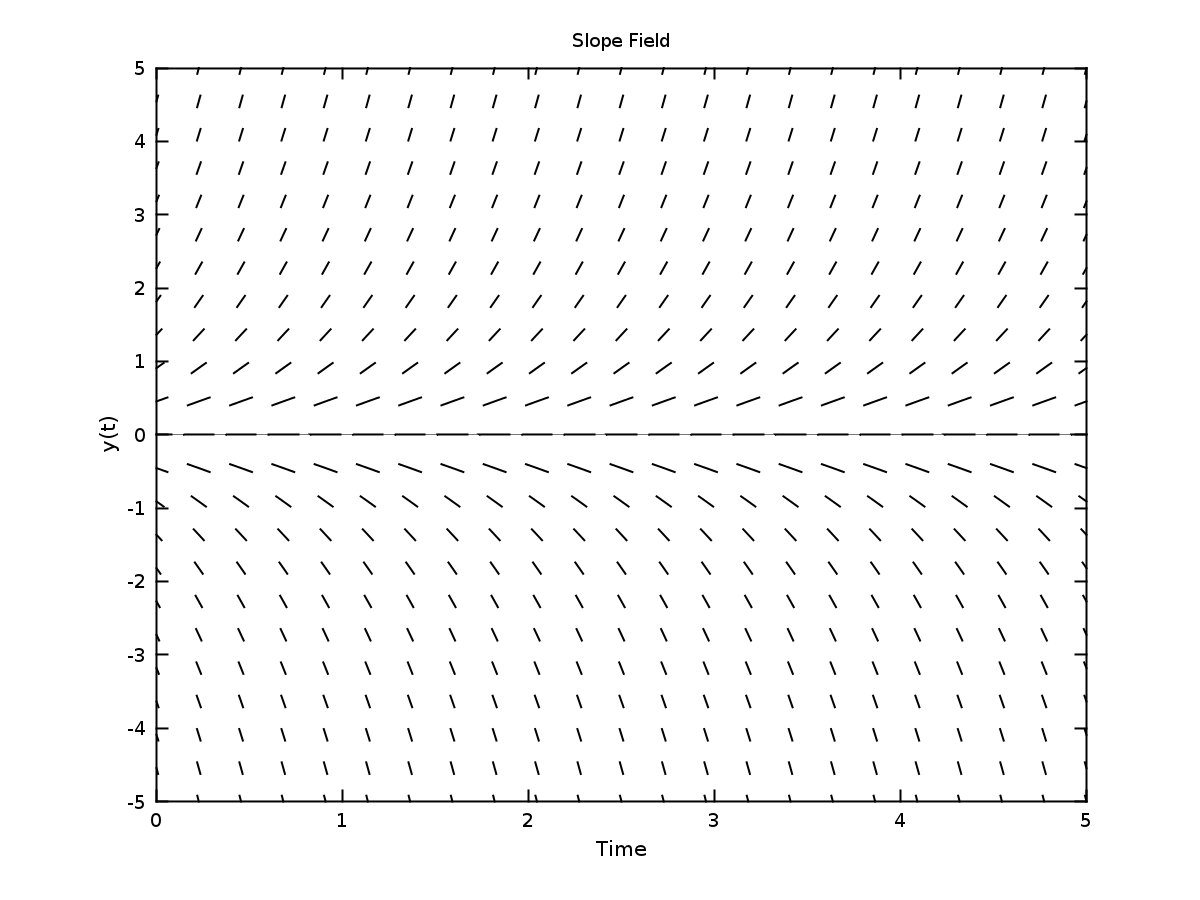
\includegraphics[height=4cm]{week1Day2SlopeField}

  A direction field is a collection of segments that indicate the
  tangent lines. 
  
\end{frame}


\begin{frame}
  \frametitle{Example}

  \vspace*{-4em}

  \begin{eqnarray*}
    y' & = & y - t
  \end{eqnarray*}

  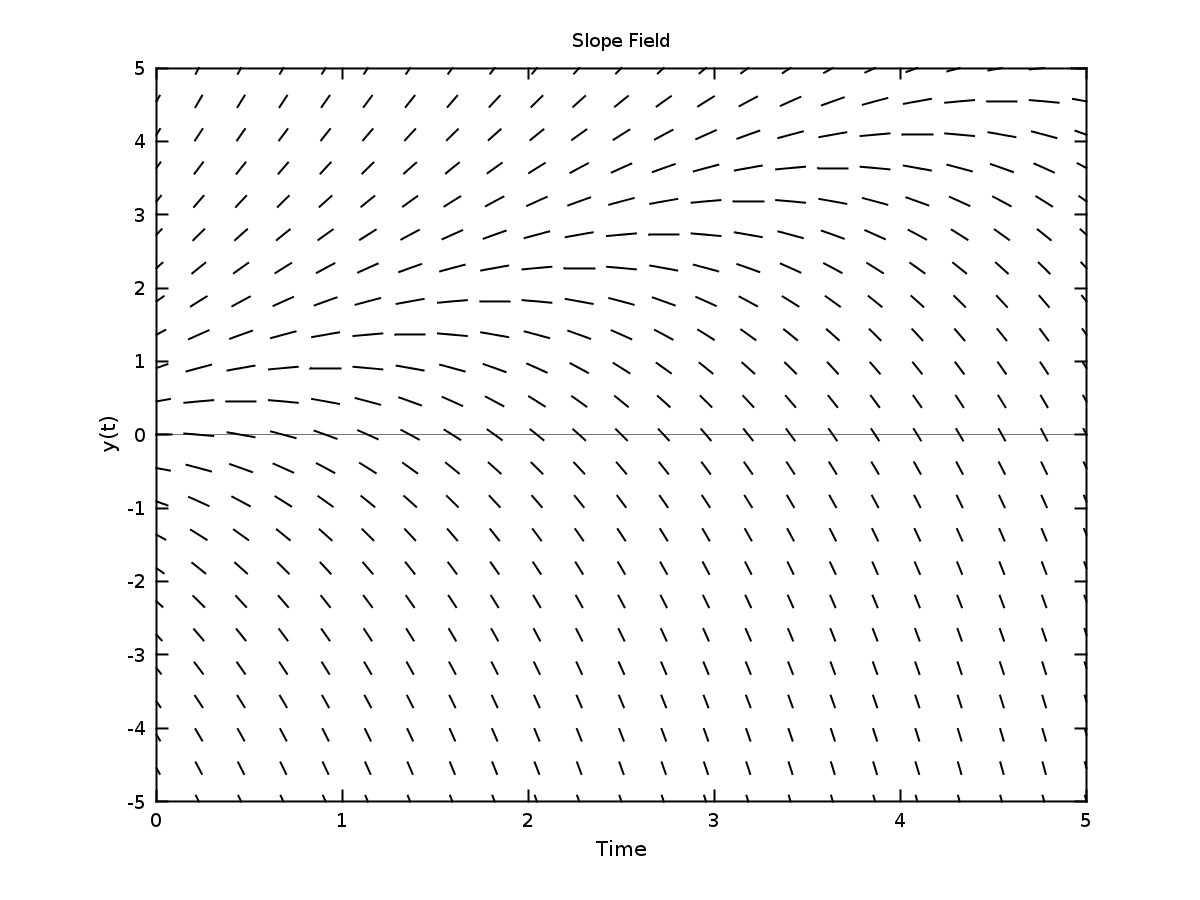
\includegraphics[height=5cm]{week1Day2SlopeField2}

  Tools:
  \begin{itemize}
  \item A ``stationary point'' is a point where $y'=0$.
  \item An isocline is a curve where $y'$ is equal to a constant.
  \end{itemize}

\end{frame}


\begin{frame}
  \frametitle{Example}

  \vspace*{-4em}

  \begin{eqnarray*}
    y' & = & y^2 - 3y
  \end{eqnarray*}

  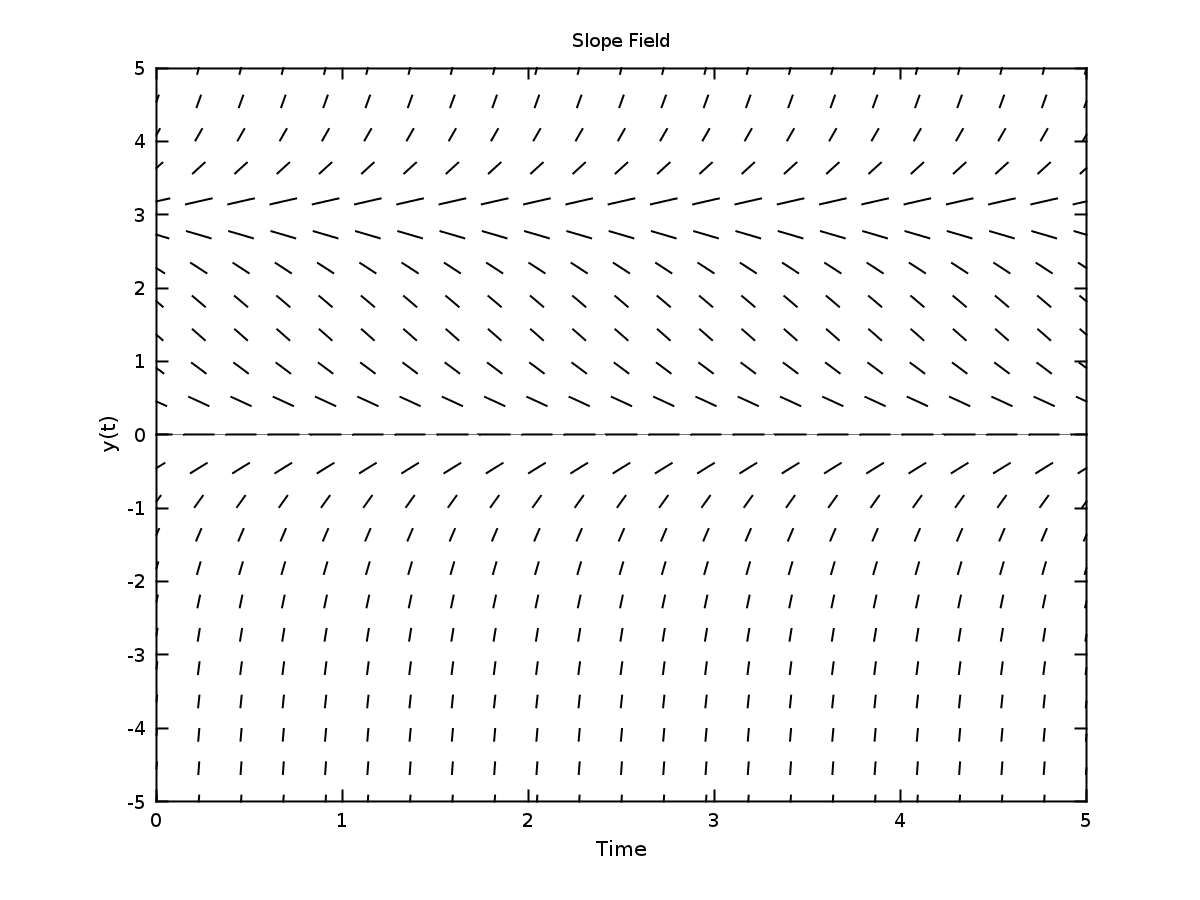
\includegraphics[height=5cm]{week1Day2SlopeField3}

  Definition: An equilibrium solution is a value for which the
  solution does not change in time.

  \uncover<2->{$y(t)=0$ and $y(t)=3$ are equilibrium solutions.}

\end{frame}

\section{Stability}

\begin{frame}
  \frametitle{Stability}

  \begin{itemize}
  \item An \textit{equilibrium solution} is \textbf{stable} if values
    of the solution tend to stay close to it as $t$ increases.
  \item An \textit{equilibrium solution} is \textbf{unstable} if
    values of the solution tend to move away from it as $t$ increases.
  \end{itemize}

  In the previous example $y=0$ is stable while $y=3$ is unstable.

\end{frame}



% LocalWords:  Clarkson pausesection hideallsubsections isocline



\title{Ordinary Differential Equations}
\subtitle{Math 232 - Week 1, Day 3}

\author{Kelly Black}
\institute{Clarkson University}
\date{2 Sep 2011}

\begin{frame}
  \titlepage
\end{frame}

\begin{frame}
  \frametitle{Outline}
  \tableofcontents[pausesection,hideallsubsections]
\end{frame}


\section{The Chain Rule}


\begin{frame}
  \frametitle{Finding Solutions}

  How do we find a solution to a DE?

  \uncover<2->{Depends!}


\end{frame}


\begin{frame}
  \frametitle{The Chain Rule}

  \begin{eqnarray*}
    \int \lp 1 + \ln(t) \rp \frac{1}{t} ~ dt & = & ?
  \end{eqnarray*}

  \uncover<2->{
    Let $u=1+\ln(t)$ then $du=\frac{1}{t}.$
  }

  \uncover<3-> {
    \begin{eqnarray*}
      \int \lp 1 + \ln(t) \rp \frac{1}{t} ~ dt & = & \int u ~ du \\
      & = & \half u^2 + C \\
      & = & \half \lp 1+\ln(t) \rp^2 + C
    \end{eqnarray*}
  }


\end{frame}

\begin{frame}
  \frametitle{The Chain Rule}

  \begin{eqnarray*}
    \int \lp 1 + \ln(t) \rp \frac{1}{t} ~ dt & = & ?
  \end{eqnarray*}

  \uncover<2->{
    Let $y=1+\ln(t)$ then $dy=\frac{1}{t}.$
  }

  \uncover<3-> {
    \begin{eqnarray*}
      \int \lp 1 + \ln(t) \rp \frac{1}{t} ~ dt & = & \int y ~ dy \\
      & = & \half y^2 + C \\
      & = & \half \lp 1+\ln(t) \rp^2 + C
    \end{eqnarray*}
  }


\end{frame}

\begin{frame}
  \frametitle{The Chain Rule}
  \begin{eqnarray*}
    \int f(y) y' ~ dt & = & \int f(y) ~ dy
  \end{eqnarray*}

  So what?

\end{frame}


\begin{frame}
  \frametitle{A Differential Equation}
  
  \begin{eqnarray*}
    y' & = & 2y
  \end{eqnarray*}

  What is $y$?

  \uncover<2->{
    Note:
    \begin{eqnarray*}
      \frac{1}{y} y' & = & 2
    \end{eqnarray*}
    I can get all the ``$y$''s on the left and the ``t''s on the
    right.
  }

\end{frame}

\section{Separable Equations}

\begin{frame}
  \frametitle{Separable Equations}

  Definition: A \textbf{separable differential equation} is an
  equation that can be expressed in the form 
  \begin{eqnarray*}
    y' & = & f(t) g(y).
  \end{eqnarray*}

  In our example:
  \begin{eqnarray*}
    y' & = & 2y \\
    f(t) & = & 2 \\
    g(y) & = & y
  \end{eqnarray*}

\end{frame}


\begin{frame}
  \frametitle{Solving Our Example}

  \begin{eqnarray*}
    y' & = & 2y \\
    \frac{1}{y} y' & = & 2, \\
    \uncover<2->{
      \int \frac{1}{y} y' ~ dt & = & \int 2 ~ dt \\
      \int \frac{1}{y} ~ dy & = & \int 2 ~ dt } \\
    \uncover<3->{
      \ln(y) & = & 2t + C } \\
    \uncover<4->{
      y & = & e^{2t + C} \\
      y & = & e^{2t} \cdot e^C \\
      y & = & k e^{2t}
    }
  \end{eqnarray*}

\end{frame}


\begin{frame}
  \frametitle{In General}

  \begin{eqnarray*}
    y' & = & f(t) g(y) \\
    \frac{1}{g(y)} y' & = & f(t) \\
    \int \frac{1}{g(y)} y' ~ dt & = & \int f(t) ~ dt \\
    \int \frac{1}{g(y)} ~ dy & = & \int f(t) ~ dt 
  \end{eqnarray*}

  \begin{itemize}
  \item Solve the integrals
  \item Solve for $y$ (if possible)
  \end{itemize}


\end{frame}


\begin{frame}
  \frametitle{Example}

  \begin{eqnarray*}
    y' & = & \frac{t}{y+y^2} \\
    \uncover<2->{
      \lp y + y^2 \rp y' & = & t } \\
    \uncover<3->{
      \int \lp y + y^2 \rp y' ~ dt & = & \int t ~ dt \\
      \int \lp y + y^2 \rp ~ dy & = & \int t ~ dt } \\
    \uncover<4->{
      \half y^2 + \frac{1}{3} y^3 & = & \half t^2 + C
    }
  \end{eqnarray*}

  \uncover<5->{
    Cannot solve explicitly for $y(t)$!
  }

\end{frame}


\begin{frame}
  \frametitle{Example}

  \begin{eqnarray*}
    y' & = & 3y + t
  \end{eqnarray*}

  \uncover<2-> { Not separable! }

\end{frame}


\begin{frame}
  \frametitle{Example}

  \begin{eqnarray*}
    y' & = & y^2 + 1 \\
    \uncover<2->{
      \frac{1}{y^2 + 1} y' & = & 1 } \\
    \uncover<3->{
      \int \frac{1}{y^2 + 1} y' ~ dt  & = & \int 1 ~ dt \\
      \int \frac{1}{y^2 + 1}  ~ dy  & = & \int 1 ~ dt } \\
    \uncover<4->{
      \arctan(y) & = & t + C } \\
    \uncover<5->{
      y & = & \tan(t+C)}
  \end{eqnarray*}

\end{frame}


\begin{frame}
  \frametitle{Example}

  \begin{eqnarray*}
    y' & = & yt + t \\
    \uncover<2->{
      y' & = & t(y+1) }\\
    \uncover<3->{
      \int \frac{1}{y+1} y' ~ dt & = & \int t ~ dt \\
      \int \frac{1}{y+1} ~ dy & = & \int t ~ dt \\
    }
    \uncover<4->{
      \ln(y+1) & = & \half t^2 + C }\\
    \uncover<5->{
      y+1 & = & e^{\half t^2 + C} \\
      y+1 & = & e^{\half t^2}e^{C} \\
      y+1 & = & k e^{\half t^2} \\
      y = ke^{\half t^2} - 1 }
  \end{eqnarray*}

\end{frame}


\begin{frame}
  \frametitle{Example}

  \begin{eqnarray*}
    y' & = & \cos(ty) 
  \end{eqnarray*}

  \uncover<2->{Not Separable!}

\end{frame}


\begin{frame}
  \frametitle{Example}

  \begin{eqnarray*}
    y' & = & \frac{t}{y}, ~~~ y(0)=2 \\
    \uncover<2->{
      y y' & = & t } \\
    \uncover<3->{
      \int y y' ~ dt & = & \int t ~ dt } \\
    \uncover<4->{
      \half y^2 & = & \half t^2 + C \\
      y^2 & = & t^2 + k } \\
    \uncover<5->{
      2^2 & = & 0 + k \\
      k   & = & 4 \\
      y & = & \pm \sqrt{t^2+4} } \\
    \uncover<6->{
      \mathrm{Must ~ be ~ positive!} \\
      y & = & \sqrt{t^2+4} }
  \end{eqnarray*}

  \uncover<6->{
    See example 4 in the book.
  }

\end{frame}


\begin{frame}
  \frametitle{Example}

  \begin{eqnarray*}
    ty' & = & y^2 t^2 + 1 \\
    \uncover<2->{
      y'  & = & y^2 t + \frac{1}{t} }
  \end{eqnarray*}

  \uncover<3->{Not separable!}

\end{frame}


\begin{frame}
  \frametitle{Example}

  \begin{eqnarray*}
    t y' & = & y^2+1 \\
    \uncover<2->{
      \frac{y'}{y^2+1} & = & \frac{1}{t} } \\
    \uncover<3->{
      \int \frac{y'}{y^2+1} ~ dt & = & \int \frac{1}{t} ~ dt \\
      \int \frac{1}{y^2+1} ~ dy & = & \int \frac{1}{t} ~ dt } \\
    \uncover<4->{
      \arctan(y) & = & \ln(t)+C } \\
    \uncover<5->{
      y & = & \tan(\ln(t)+C)}
  \end{eqnarray*}





\end{frame}


\begin{frame}
  \frametitle{Example}

  \vspace*{-3em}
  \begin{eqnarray*}
    y' & = & \sec(y) t^2 + \sec(y) \sin(4t) \\
    \uncover<2->{
      y' & = & \sec(y) \lp t^2 + \sin(4t) \rp } \\
    \uncover<3->{
      \frac{y'}{\sec(y)} & = & t^2 + \sin(4t) } \\
    \uncover<4->{
      \int \frac{y'}{\sec(y)} ~ dt & = & \int t^2 + \sin(4t) ~ dt \\
      \int \frac{1}{\sec(y)} ~ dy & = & \int t^2 + \sin(4t) ~ dt }\\
    \uncover<5->{
      \int \cos(y) ~ dy & = & \int t^2 + \sin(4t) ~ dt } \\ 
    \uncover<6->{
      \sin(y) & = & \frac{1}{3} t^3 - \frac{1}{4} \cos(4t) + C } \\
    \uncover<7->{
      y & = & \arcsin\lp\frac{1}{3} t^3 - \frac{1}{4} \cos(4t) + C\rp } \\
  \end{eqnarray*}

  \uncover<8->{This is problematic!}

\end{frame}
 


% LocalWords:  Clarkson pausesection hideallsubsections




% %%%%%%%%%%%%%%%%%%%%%%%%%%%%%%%%%%%%%%%%%%%%%%%%%%%%%%%%%%%%

\part{Linear-Equations}
\lecture{Linear Equations}{Linear-Equations}
\section{Linear Equations}


\title{Ordinary Differential Equations}
\subtitle{Math 232 - Week 2, Day 1}
\date{3 Sep 2012}

\begin{frame}
  \titlepage
\end{frame}

\begin{frame}
  \frametitle{Outline}
  \tableofcontents[pausesection,hideothersubsections]
\end{frame}


\subsection{Linear Equations}


\iftoggle{clicker}{%
\begin{frame}
  \frametitle{Clicker Quiz}
    
      \ifnum\value{clickerQuiz}=1{%

       Determine the solution to the differential equation
       \begin{eqnarray*}
         y' & = & y + 1.
       \end{eqnarray*}

       \vfill

       \begin{tabular}{l@{\hspace{3em}}l}
         A: & $y=-1 + e^t + C$. \\
         B: & $y=-1+ke^t$. \\
         C: & $y=ke^t$. \\
         D: & $y=1+ke^t$. \\
       \end{tabular}
     }\fi

     \ifnum\value{clickerQuiz}=2{%
       Determine the solution to the differential equation
       \begin{eqnarray*}
         y' & = & ty.
       \end{eqnarray*}

       \vfill

       \begin{tabular}{l@{\hspace{3em}}l}
         A: & $y=\half ke^{t^2}$. \\
         B: & $y=ke^{t}$. \\
         C: & $y=ke^{t^2/2}$. \\
         D: & $y=e^{t^2/2} + C$. \\
       \end{tabular}
     }\fi

      \ifnum\value{clickerQuiz}=3{%
       Determine the solution to the differential equation
       \begin{eqnarray*}
       y' & = & -2t^2y? 
       \end{eqnarray*}

       \vfill

       \begin{tabular}{l@{\hspace{3em}}l}
         A: & $y=e^{\frac{-2t^3}{3}}+C$. \\
         B: & $y=-\dfrac{2t^3}{3}+C$. \\
         C: & $y=\sqrt[3]{\half t^2+C}$. \\
         D: & $y= k e^{\frac{-2t^3}{3}}$. \\
       \end{tabular}
     }\fi

    \vfill
    \vfill
    \vfill

\end{frame}
}



\begin{frame}
  \frametitle{Linear Equations}

  If we have variables $x_1$, $x_2$, \ldots, $x_n$ then an equation of
  the form
  \begin{eqnarray*}
    a_1 x_1 + a_2 x_2 + \cdots + a_n x_n & = & c,
  \end{eqnarray*}
  where $a_1$, $a_2$, \ldots, $a_n$, and $c$ are constants, is a
  \textbf{linear equation}.

  if $c$ is zero the equation is \textbf{homogeneous}.

\end{frame}


\begin{frame}
  \frametitle{Linear Equations}

  \begin{eqnarray*}
    3 x_1 + 4 x_2 = 5 & & \uncover<2->{\mathrm{Linear}} \\
    3 x_1 + 4 x^3_2 = 5 & & \uncover<3->{\mathrm{Not~Linear}} \\
    3 \sqrt{x_1} + 4 x_2 = 5 & & \uncover<4->{\mathrm{Not~Linear}} \\
  \end{eqnarray*}


\end{frame}


\begin{frame}
  \frametitle{Linear Differential Equations}

  In the context of DEs an equation is linear if it is in the form
  \begin{eqnarray*}
    a_0(t) y(t) + a_1(t) \frac{d}{dt}y(t) + \cdots +
    a_n(t) \frac{d^n}{dt^n}y(t) & = & f(t).
  \end{eqnarray*}

  if $f(t)$ is zero the equation is \textbf{homogeneous}.

\end{frame}


\begin{frame}
  \frametitle{Example}

  \vspace*{-3em}
  \begin{eqnarray*}
    3t y + y' - \sin(t) y'' & = & \ln(t)
  \end{eqnarray*}
  \centerline{\color{red}{\uncover<2->{Linear, variable coefficients, nonhomogeneous!}}}

  \begin{eqnarray*}
    3t \sqrt{y} + y' - \sin(t) y'' & = & \ln(t)
  \end{eqnarray*}
  \centerline{\color{red}{\uncover<3->{Not Linear, variable coefficients, nonhomogeneous!}}}

  \begin{eqnarray*}
    3 y' -y'' & = & 4 y
  \end{eqnarray*}
  \centerline{\color{red}{\uncover<4->{Linear, constant coefficients, homogeneous!}}}
  \centerline{\uncover<5->{Linear, \textbf{constant coefficient}, and homogeneous}}

  Recognizing the form is the hardest part!

\end{frame}

\subsection{Solutions to Differential Equations}

\begin{frame}
  \frametitle{Solutions to Differential Equations}

  If an equation is linear and homogeneous then:
  \begin{itemize}
  \item If $y_1(t)$ is a solution, and
  \item if $y_2(t)$ is a solution
  \end{itemize}

  then,
  \begin{eqnarray*}
    y_1(t) + y_2(t)
  \end{eqnarray*}
  is a solution.

  Also if $C_1$ and $C_2$ are constants then
  \begin{eqnarray*}
    C_1 y_1(t) + C_2 y_2(t)
  \end{eqnarray*}
  is also a solution.

  Because:
  \begin{eqnarray*}
    \frac{d}{dt} \lp C_1 y_1(t) + C_2 y_2(t) \rp & = &
    C_1 y_1'(t) + C_2 y_2'(t)
  \end{eqnarray*}


\end{frame}


\begin{frame}
  \frametitle{Example}

  Solutions to the second order equation,
  \begin{eqnarray*}
    y'' + y & = & 0,
  \end{eqnarray*}
  are
  \begin{eqnarray*}
    y_1(t) & = & \cos(t) \\
    y_2(t) & = & \sin(t).
  \end{eqnarray*}

  \uncover<2->{%

    Because:
    \begin{eqnarray*}
      y''_1(t) & = & -\cos(t), \\
      \Rightarrow y''_1(t) + y_1(t) & = & -\cos(t)+\cos(t), \\
      y''_2(t) & = & -\sin(t), \\
      \Rightarrow y''_2(t) + y_2(t) & = & -\sin(t)+\sin(t).
    \end{eqnarray*}

  }

\end{frame}

\begin{frame}
  \frametitle{Example}

  Also:
  \begin{eqnarray*}
    y(t) & = & C_1 \cos(t) + C_2 \sin(t), \\
    y'(t) & = & -C_1 \sin(t) + C_2 \cos(t), \\
    y''(t) & = & -C_1 \cos(t) - C_2 \sin(t), \\
    y''(t) + y(t) & = & -C_1 \cos(t) - C_2 \sin(t) + C_1 \cos(t) + C_2 \sin(t) \\
    & = & 0
  \end{eqnarray*}


\end{frame}


\iftoggle{clicker}{%
\begin{frame}
  \frametitle{Clicker Quiz}
    
      \ifnum\value{clickerQuiz}=1{%

        The function $y=-2e^{3t} + 4 e^{2t}$ is a solution to the
        equation
        \begin{eqnarray*}
          y'' - 5 y' + 6y & = & 0.
        \end{eqnarray*}

        Is the function $y=5e^{3t} - e^{2t}$ also a solution?

       \vfill

       \begin{tabular}{l@{\hspace{3em}}l}
         A: & Yes, it is a solution. \\
         B: & No, it is not a solution.
       \end{tabular}

     }\fi

     \ifnum\value{clickerQuiz}=2{%

        The function $y=2e^{3t}$ is a solution to the
        equation
        \begin{eqnarray*}
          y' & = & y^2.
        \end{eqnarray*}

        Is the function $y=50e^{3t}$ also a solution?

       \vfill

       \begin{tabular}{l@{\hspace{3em}}l}
         A: & Yes, it is a solution. \\
         B: & No, it is not a solution.
       \end{tabular}

     }\fi

      \ifnum\value{clickerQuiz}=3{%
      The function $y=-\frac{1}{t+3}$ is a solution to the
        equation
        \begin{eqnarray*}
          y' & = & y^2.
        \end{eqnarray*}

        Is the function $y=\frac{2}{t+3}$ also a solution?

       \vfill

       \begin{tabular}{l@{\hspace{3em}}l}
         A: & Yes, it is a solution. \\
         B: & No, it is not a solution.
       \end{tabular}

     }\fi

    \vfill
    \vfill
    \vfill

\end{frame}
}



\subsection{Nonhomogeneous Solutions and Homogeneous Solutions}


\begin{frame}
  \frametitle{It Gets Worse!}

  Suppose that an equation is linear but not homogeneous,
  \begin{eqnarray*}
    a_0(t) y_p(t) + a_1(t) \frac{d}{dt} y_p(t) + \cdot + a_n(t) \frac{d^n}{dt^n} y_p(t) & = & f(t)
  \end{eqnarray*}
  where $f(t)$ is not zero.

  The homogeneous version is
  \begin{eqnarray*}
    a_0(t) y_h(t) + a_1(t) \frac{d}{dt} y_h(t) + \cdot + a_n(t) \frac{d^n}{dt^n} y_h(t) & = & 0.
  \end{eqnarray*}

  then $y_p(t)+y_h(t)$ is a solution to the original equation!


\end{frame}


\begin{frame}
  \frametitle{Example}

  \begin{eqnarray*}
    y' - y & = & t
  \end{eqnarray*}

  Particular: $y_p = -t-1$

  \begin{eqnarray*}
    y'_p & = & -1, \\
    -1 - (-t -1) & = & t.
  \end{eqnarray*}

  Homogeneous: $y_h = k e^t$

  \begin{eqnarray*}
    y'_h - y_h & = & 0, \\
    y'_h & = & k e^t, \\
    k e^t - k e^t & = & 0.
  \end{eqnarray*}

\end{frame}

\begin{frame}
  \frametitle{Example}

  \begin{eqnarray*}
    y' - y & = & t
  \end{eqnarray*}

  \begin{eqnarray*}
    y & = & -t - 1 + ke^t, \\
    y' & = & -1 + ke^t, \\
    -1-ke^t - (-t-1-ke^t) & = & t.
  \end{eqnarray*}

\end{frame}


\begin{frame}
  \frametitle{Example}

  \begin{eqnarray*}
    y'' + 4y & = & t.
  \end{eqnarray*}

  \begin{eqnarray*}
    y_p & = & \frac{1}{4} t, \\
    y'_p & = & \frac{1}{4}, \\
    y''_p & = & 0, \\
    0 + 4\frac{1}{4} t & = & t
  \end{eqnarray*}
\end{frame}

\begin{frame}
  \frametitle{Example - Homogeneous Part}

  \begin{eqnarray*}
    y''_h + 4y_h & = & 0, \\
    y_h & = & C_1 \cos(2t) + C_2 \sin(2t), \\
    y'_h & = & -2 C_1 \sin(2t) + 2 C_2 \cos(2t), \\
    y''_h & = & -4 C_1 \cos(2t) - 4 C_2 \sin(2t),
  \end{eqnarray*}
  \begin{eqnarray*}
    -4 C_1 \cos(2t) - 4 C_2 \sin(2t) + 4\lp C_1 \cos(2t) + C_2 \sin(2t) \rp & = & 0.
  \end{eqnarray*}

\end{frame}


\begin{frame}
  \frametitle{Example - Bring them together}

  \begin{eqnarray*}
    y & = & y_p + y_h \\
    & = & \frac{1}{4} t + C_1 \cos(2t) + C_2 \sin(2t), \\
    y' & = & \frac{1}{4} - 2 C_1 \sin(2t) + 2 C_2 \cos(2t), \\
    y'' & = & - 4 C_1 \cos(2t) - 4 C_2 \sin(2t),
  \end{eqnarray*}

  \begin{eqnarray*}
    - 4 C_1 \cos(2t) - 4 C_2 \sin(2t) + 4 \lp \frac{1}{4} t + C_1 \cos(2t) + C_2 \sin(2t) \rp & = & t
  \end{eqnarray*}

\end{frame}


\begin{frame}
  \frametitle{Example}

  \begin{eqnarray*}
    y' - 3y & = & 4
  \end{eqnarray*}

  \begin{eqnarray*}
    y_p & = & -\frac{4}{3}, \\
    y_h & = & k e^{3t}
  \end{eqnarray*}

  \begin{eqnarray*}
    y & = & -\frac{4}{3} + k e^{3t}, \\
    y' & = & 3 k e^{3t}, \\
    3 k e^{3t} - 3 \lp -\frac{4}{3} + k e^{3t} \rp & = & 4
  \end{eqnarray*}


\end{frame}


\begin{frame}
  \frametitle{Example}

  \begin{eqnarray*}
    y' - 3ty & = & t^3
  \end{eqnarray*}

  \begin{eqnarray*}
    y_p & = & -\frac{1}{3} t^2 - \frac{2}{9}, \\
    y_h & = & k e^{\frac{3}{2}t^2}
  \end{eqnarray*}

  \begin{eqnarray*}
    y & = & -\frac{1}{3} t^2 - \frac{2}{9} + k e^{\frac{3}{2}t^2} \\
    y' & = & -\frac{2}{3} t + 3t k e^{\frac{3}{2}t^2}
  \end{eqnarray*}

  Substituting back into the equation we get
  \begin{eqnarray*}
    -\frac{2}{3} t + 3t k e^{\frac{3}{2}t^2} - 3t \lp -\frac{1}{3} t^2 - \frac{2}{9} + k e^{\frac{3}{2}t^2} \rp & = & t^3.
  \end{eqnarray*}

\end{frame}




\part{First-Order-Linear-Equations}
\lecture{First Order Linear Equations}{First-Order-Linear-Equations}
\section{First Order Linear Equations}

\title{Ordinary Differential Equations}
\subtitle{Math 232 - Week 2, Day 2}
\date{4 Sep 2012}

\begin{frame}
  \titlepage
\end{frame}

\begin{frame}
  \frametitle{Outline}
  \tableofcontents[pausesection,hideothersubsections]
\end{frame}


\subsection{First Order Linear Equations}

\iftoggle{clicker}{%

  \begin{frame}
    \frametitle{Clicker Quiz}

      \ifnum\value{clickerQuiz}=1{%

        Which differential equation is a linear equation?

       \vfill

       \begin{tabular}{l@{\hspace{3em}}l}
         A: & $y'=y^2$. \\
         B: & $y'' + 3y'-2y=0$. \\
         C: & $y'+\sqrt{y}=\sin(t)$. \\
         D: & $y' + \cos(t)y  =  \ln(t)$. \\
         E: & A and B. \\
         F: & B and D.
       \end{tabular}

     }\fi

     \ifnum\value{clickerQuiz}=2{%

        Which differential equation is a linear equation?

       \vfill

       \begin{tabular}{l@{\hspace{3em}}l}
         A: & $y'=3y$. \\
         B: & $y'' + 3\sin(t)y'-2y=0$. \\
         C: & $y''+ y^2 =\sin(t)$. \\
         D: & $y' + y y'  =  \ln(t)$. \\
         E: & A and B. \\
         F: & A and D.
       \end{tabular}


     }\fi
    

      \ifnum\value{clickerQuiz}=3{%

      }\fi

    \vfill
    \vfill
    \vfill

  \end{frame}

}


\begin{frame}
  \frametitle{Another ``Special Form''}

  \begin{eqnarray*}
    y' + p(t) y & = & f(t)
  \end{eqnarray*}

  read pages 63-66 

  I will only cover integrating factors in class.

\end{frame}

\subsection{Product Rule}

\begin{frame}
  \frametitle{The Product Rule}

  \begin{eqnarray*}
    \frac{d}{dt} \lp u v \rp & = & u' v + u v'
  \end{eqnarray*}

\end{frame}


\begin{frame}
  \frametitle{Example}

  \begin{eqnarray*}
    y ' & = & - y + t \\
    \uncover<2->{ y' + y & = & t} \\
    \uncover<3->{y' e^t + y e^ t & = & t e^t } \\
    \uncover<4->{\deriv{~}{t} \lp y e^t \rp & = & t e^t } \\
    \uncover<5->{y e^t  & = & \int t e^t ~ dt } \\
    \uncover<6->{y e^t  & = & t e^t - e^t + C } \\
    \uncover<7->{ y & = & t -1 + Ce^{-t}}
  \end{eqnarray*}

  \uncover<8->{How did I know how to do this?}


\end{frame}


\subsection{Integrating Factors}

\begin{frame}
  \frametitle{Let's Backup}

  \begin{eqnarray*}
    y' + p(t) y & = & f(t) \\
    e^{G(t)} y' + p(t) e^{G(t)} y & = & e^{G(t)} f(t)
  \end{eqnarray*}


\end{frame}



\begin{frame}
  \frametitle{Product Rule Redux}

  \begin{eqnarray*}
    \frac{d}{dt} \lp e^{G(t)} \rp & = & G'(t) e^{G(t)} 
  \end{eqnarray*}

  Let
  \begin{eqnarray*}
    G'(t) & = & p(t) \\
    \Rightarrow G(t) & = & \int p(t) ~ dt.
  \end{eqnarray*}


\end{frame}


\begin{frame}
  \frametitle{Product Rule Redux}

  \begin{eqnarray*}
    \frac{d}{dt} \lp e^{G(t)} y \rp & = & e^{G(t)} y' + G'(t) e^{G(t)} y \\
    & = & e^{G(t)} y' + p(t) e^{G(t)} y \\
    & = & e^{G(t)} \lp y' + p(t) y \rp \\
    & = & f(t) e^{G(t)}
  \end{eqnarray*}

  or
  \begin{eqnarray*}
    e^{G(t)} y & = & \int f(t) e^{G(t)} ~ dt
  \end{eqnarray*}
  \textit{Hope and pray!}

\end{frame}


\subsection{Examples}

\begin{frame}
  \frametitle{Example}

  \vspace*{-3em}
  \begin{eqnarray*}
    y' + 2y & = & t \\
    p(t) & = & 2, \\
    \int 2 ~ dt & = & 2t + K, \\
    e^{2t} & & 
  \end{eqnarray*}

  \begin{eqnarray*}
    e^{2t} y' + 2 e^{2t} y & = & t e^{2t}, \\
    \frac{d}{dt} \lp e^{2t} y \rp & = & t e^{2t} \\
    e^{2t} y & = & \int t e^{2t} ~ dt \\
    e^{2t} y & = & \half t e^{2t} - \frac{1}{4} e^{2t} + C \\
    y & = & \half t - \frac{1}{4} + C e^{-2t}
  \end{eqnarray*}

\end{frame}


\iftoggle{clicker}{%
\begin{frame}
  \frametitle{Clicker Quiz}
    
      \ifnum\value{clickerQuiz}=1{%

        What is the integrating factor for the equation
        \begin{eqnarray*}
          y' & = & ty + 1 ?
        \end{eqnarray*}

       \vfill

       \begin{tabular}{l@{\hspace{3em}}l}
         A: & $e^{t}$. \\
         B: & $e^{-t}$. \\
         C: & $e^{t^2/2}$. \\
         D: & $e^{-t^2/2}$. \\
       \end{tabular}

     }\fi

     \ifnum\value{clickerQuiz}=2{%

        What is the integrating factor for the equation
        \begin{eqnarray*}
          y' & = & ty + t^4 ?
        \end{eqnarray*}

       \vfill

       \begin{tabular}{l@{\hspace{3em}}l}
         A: & $e^{t}$. \\
         B: & $e^{-t}$. \\
         C: & $e^{t^2/2}$. \\
         D: & $e^{-t^2/2}$. \\
       \end{tabular}


     }\fi

      \ifnum\value{clickerQuiz}=3{%

     }\fi

    \vfill
    \vfill
    \vfill

\end{frame}

}


\begin{frame}
  \frametitle{Example}

  \vspace*{-3em}
  \begin{eqnarray*}
    y' & = & ty + t^3 \\
    y' - ty & = & t^3 \\
    p(t) & = & -t, \\
    \int -t ~ dt & = & -\half t^2 + K \\
    e^{-\half t^2} & & 
  \end{eqnarray*}

  \begin{eqnarray*}
    y' e^{-\half t^2} - t e^{-\half t^2} y & = & t^3 e^{-\half t^2} \\
    \frac{d}{dt} \lp y e^{-\half t^2} \rp & = & \int t^3 e^{-\half t^2} ~ dt \\
    y e^{-\half t^2} & = & -t^2 e^{-\half t^2} - 2 e^{-\half t^2} + C \\
    y & = & -t^2 - 2 + C e^{\half t^2}
  \end{eqnarray*}

\end{frame}


\iftoggle{clicker}{%
\begin{frame}
  \frametitle{Clicker Quiz}
    
      \ifnum\value{clickerQuiz}=1{%

        What is the integrating factor for the equation
        \begin{eqnarray*}
          y' & = & -\frac{4}{t} y + 4 ?
        \end{eqnarray*}

       \vfill

       \begin{tabular}{l@{\hspace{3em}}l}
         A: & $4t$. \\
         B: & $4\ln(t)$. \\
         C: & $t^4$. \\
         D: & $t^{-4}$. \\
       \end{tabular}

     }\fi

     \ifnum\value{clickerQuiz}=2{%

        What is the integrating factor for the equation
        \begin{eqnarray*}
          y' & = & -\frac{4}{t} y + t^3?
        \end{eqnarray*}

       \vfill

       \begin{tabular}{l@{\hspace{3em}}l}
         A: & $t^{-4}$. \\
         B: & $t^4$. \\
         C: & $4\ln(t)$. \\
         D: & $4t$. \\
       \end{tabular}


     }\fi

      \ifnum\value{clickerQuiz}=3{%

     }\fi

    \vfill
    \vfill
    \vfill

\end{frame}

}


\begin{frame}
  \frametitle{Example}

  \begin{eqnarray*}
    y' & = & -\frac{4}{t} y + 4 t \\
    y' + \frac{4}{t} y & = & 4 t \\
    p(t) & = & \frac{4}{t} \\
    \int \frac{4}{t} ~ dt & = & 4 \ln(t) + K \\
    e^{4 \ln(t) } & = & t^4
  \end{eqnarray*}

\end{frame}

\begin{frame}
  \frametitle{Example - continues}

  \begin{eqnarray*}
    t^4 y' + 4t^3& = & 4 t^5 \\
    \frac{d}{dt} \lp t^4 y \rp & = & 4 t^5 \\
    t^4 y & = & \int 4 t^5 ~ dt \\
    t^4 y & = & \frac{4}{6} t^6 + C \\
    y & = & \frac{2}{3} t^2 + \frac{C}{t^4}
  \end{eqnarray*}

\end{frame}



\begin{frame}
  \frametitle{Example}

  \vspace*{-3em}
  \begin{eqnarray*}
    y' & = & -\frac{1}{t} y + \frac{1}{t^2 -1} \\
    y' + \frac{1}{t} y & = & \frac{1}{t^2 -1} \\
    p(t) & = & \frac{1}{t} \\
    \int \frac{1}{t} ~ dt & = & \ln(t) + k \\
    e^{\ln(t)} & = & t
  \end{eqnarray*}

  \begin{eqnarray*}
    t y' + y & = & \frac{t}{t^2-1} \\
    \frac{d}{dt} \lp t y \rp & = & \frac{t}{t^2-1} \\
    t y & = & \int \frac{t}{t^2-1} ~ dt.
  \end{eqnarray*}

\end{frame}


\begin{frame}
  \frametitle{Solving the Integral}

  Let $u=t^2-1$, and $du=2t$:
  \begin{eqnarray*}
    ty & = & \int \half \frac{1}{u} ~ du, \\
    t y & = & \half \ln(u) + C, \\
    t y & = & \half \ln \lp t^2 - 1 \rp + C, \\
    y & = & \frac{\ln\lp t^2-1 \rp}{t} + \frac{C}{t}.
  \end{eqnarray*}

\end{frame}


\begin{frame}
  \frametitle{Partial Fractions}

  \vspace{-3em}
  \begin{eqnarray*}
    \frac{t}{(t-1)(t+1)} & = & \frac{A}{t-1} + \frac{B}{t+1} \\
    t & = & A(t+1) + B(t-1)
  \end{eqnarray*}

  Let $t=-1$
  \begin{eqnarray*}
    -1 & = & -2B, \\
    B & = & \half
  \end{eqnarray*}

  Let $t=1$
  \begin{eqnarray*}
    1 & = & 2A \\
    A & = & \half
  \end{eqnarray*}

  \begin{eqnarray*}
    t y & = & \int \frac{\half}{t-1} + \frac{\half}{t+1} ~ dt \\
    t y & = & \half \ln(t-1) + \half \ln(t+1) \\
    y &  = & \frac{\half \ln(t-1) + \half \ln(t+1)}{t}
  \end{eqnarray*}


\end{frame}


\begin{frame}
  \frametitle{Example}

  \begin{eqnarray*}
    y' & = & \cos(t) y - \cos(t) \\
    \uncover<2->{ y' & = & \cos(t) \lp y-1 \rp,} \\
    \uncover<3->{\frac{y'}{y-1} & = & \cos(t) \\
      \ln(y-1) & = & \sin(t) + C \\
      y - 1 & = & k e^{\sin(t)} \\
      y & = & 1 + ke^{\sin(t)} }
  \end{eqnarray*}

\end{frame}


\begin{frame}
  \frametitle{Example}

  \begin{eqnarray*}
    y' & = & y^2 + 1, \\
    \uncover<2->{ \frac{y'}{y^2+1} & = & 1,} \\
    \uncover<3->{\int \frac{y'}{y^2+1} ~ dt  & = & \int 1 ~ dt, \\
      \arctan(y) & = & t + C \\
      y  & = & \tan(t+C) }
  \end{eqnarray*}

\end{frame}



% LocalWords:  Clarkson pausesection hideothersubsections


\part{Growth-and-Decay}
\lecture{Growth and Decay}{Growth-and-Decay}
\section{Growth and Decay}

\title{Ordinary Differential Equations}
\subtitle{Math 232 - Week 2, Day 3}
\date{7 Sep 2012}

\begin{frame}
  \titlepage
\end{frame}

\begin{frame}
  \frametitle{Outline}
  \tableofcontents[pausesection,hideothersubsections]

  (Section 2.3 in book)
\end{frame}


\subsection{Growth and Decay}



\iftoggle{clicker}{%
\begin{frame}
  \frametitle{Clicker Quiz}
    
      \ifnum\value{clickerQuiz}=1{%

        What is the integrating factor for the equation
        \begin{eqnarray*}
          y' & = & \frac{2}{t} y + t ?
        \end{eqnarray*}

       \vfill

       \begin{tabular}{l@{\hspace{3em}}l}
         A: & $t^{2}$. \\
         B: & $-2\ln(t)$. \\
         C: & $e^{-t^2}$. \\
         D: & $t^{-2}$. \\ 
       \end{tabular}

     }\fi

     \ifnum\value{clickerQuiz}=2{%

        What is the integrating factor for the equation
        \begin{eqnarray*}
          y' & = & \frac{7}{t} y + 1?
        \end{eqnarray*}

       \vfill

       \begin{tabular}{l@{\hspace{3em}}l}
         A: & $t^{7}$. \\
         B: & $-7\ln(t)$. \\
         C: & $e^{-t^7}$. \\
         D: & $t^{-7}$. \\
       \end{tabular}


     }\fi

      \ifnum\value{clickerQuiz}=3{%
        What is the integrating factor for the equation
        \begin{eqnarray*}
          y' & = & 2 t y + 12t^2e^{t^2}?
        \end{eqnarray*}

       \vfill

       \begin{tabular}{l@{\hspace{3em}}l}
         A: & $t^{2}$. \\
         B: & $-t^{2}$. \\
         C: & $e^{-t^2}$. \\
         D: & $e^{t^2}$. \\
       \end{tabular}

     }\fi

    \vfill
    \vfill
    \vfill

\end{frame}

}


\begin{frame}
  \frametitle{Growth and Decay}

  \begin{quote}
    Rate of growth is proportional to the amount that is present.
  \end{quote}

  \begin{tabular}{rrcl}
    & amount present & $=$ & $y$ \\
    \uncover<2->{& rate of growth & $=$ & $y'$} \\
    \uncover<3->{$\Rightarrow$ & There is a constant where & & $y'=ky$.}
  \end{tabular}


\end{frame}


\begin{frame}
  \frametitle{Growth, $k>-$}

  \includegraphics<1>[height=6cm]{img/week2GrowthSlopeField}
  \includegraphics<2>[height=6cm]{img/week2GrowthSlopeFieldSolutions}


\end{frame}


\begin{frame}
  \frametitle{Decay, $k<0$}

  \includegraphics<1>[height=6cm]{img/week2DecaySlopeField}
  \includegraphics<2>[height=6cm]{img/week2DecaySlopeFieldSolutions}


\end{frame}


\begin{frame}
  \frametitle{Solution}

  \begin{eqnarray*}
    y' & = & k y \\
    \frac{y'}{y} & = & k \\
    \int \frac{y'}{y} ~ dt & = & \int k ~ dt \\
    \ln(y) & = & kt + C \\
    y & = & e^{kt+C} \\
    y & = & A e^{kt}
  \end{eqnarray*}

  where $A$ is a constant.

  Solution decays if $k<0$

  Solution grows if $k>0$

\end{frame}

\subsection{Examples}

\begin{frame}
  \frametitle{Example - Radioactive Decay}

  The rate of decay of the radioactive material is proportional to the
  amount present. A sample of wood is found at the site. It contains
  15\% of what modern wood contains of C-14. The half-life of C-14 is
  5600 years. How old is the wood?

\end{frame}


\begin{frame}

  Let $Q$ be the amount of C-14 in the sample.

  \begin{eqnarray*}
    Q' & = & kQ \\
    Q & = & A e^{kt}
  \end{eqnarray*}

  \uncover<2->{In 5600 years $Q$ is cut in half.}

  \uncover<3->{Let $t=0$ be the start time:}
    \begin{eqnarray*}
      \uncover<4->{Q(t) & = & A e^{kt} }\\
      \uncover<5->{Q(0) & = & A }\\
      \uncover<6->{Q(5600) & = & \half A } \\
      \uncover<7->{Q(5600) & = & A e^{k 5600} }\\
      \uncover<8->{\half & = & e^{k 5600} }\\
      \uncover<9->{\ln\lp\half\rp & = & k 5600 }\\
      \uncover<10->{k & = & \frac{\ln\lp\half\rp}{5600} }\\
  \end{eqnarray*}

\end{frame}


\begin{frame}

  \begin{eqnarray*}
    Q(t) & = & A e^{\frac{\ln\lp\half\rp}{5600}t} \\
    \uncover<2->{Q(T) & = & 0.15 A } \\
    \uncover<3->{.15A & = & A e^{\frac{\ln\lp\half\rp}{5600}T} }\\
    \uncover<4->{.15 & = & e^{\frac{\ln\lp\half\rp}{5600}T} }\\
    \uncover<4->{\ln(.15) & = & \frac{\ln\lp\half\rp}{5600}T }\\
    \uncover<4->{T & = & \frac{\ln(.15) 5600}{\ln\lp\half\rp} ~ \mathrm{years}}
  \end{eqnarray*}

\end{frame}




\begin{frame}
  \frametitle{Continual Interest}

  The rate of change of the balance in a bank account is proportional
  to the amount of money present.

  Let $A(t)$ be the amount of money.

  \uncover<2->{%

    \begin{eqnarray*}
      A' & = & r A \\
      A(0) & = & A_0 \\
      A(t) & = & k e^{rt} \\
      A_0 & = & k e^0 \\
      k  & = & A_0 \\
      A(t) & = & A_0 e^{rt}
    \end{eqnarray*}

  }

\end{frame}



\iftoggle{clicker}{%
\begin{frame}
  \frametitle{Clicker Quiz}
    
      \ifnum\value{clickerQuiz}=1{%

        A bank promises 5\% interest compounded annually. What is the governing equation?

       \vfill

       \begin{tabular}{l@{\hspace{3em}}l}
         A: & $A' = A_0 e^{0.05t}$. \\
         B: & $A'= 0.05A$. \\
         C: & $A'=-0.05A$. \\
         D: & What is up with Hank Williams?
       \end{tabular}

     }\fi

     \ifnum\value{clickerQuiz}=2{%

        A bank promises 5\% interest compounded annually. What is the governing equation?

       \vfill

       \begin{tabular}{l@{\hspace{3em}}l}
         A: & $A' = A_0 e^{0.05t}$. \\
         B: & $A'= 0.05A$. \\
         C: & $A'=-0.05A$. \\
         D: & What is up with Hank Williams?
       \end{tabular}


     }\fi

      \ifnum\value{clickerQuiz}=3{%
      A bank promises 8\% interest compounded annually. 
      What is the governing equation?

       \vfill

       \begin{tabular}{l@{\hspace{3em}}l}
         A: & $A' = A_0 e^{0.08t}$. \\
         B: & $A'= 0.08A$. \\
         C: & $A'=-0.08A$. \\
         D: & $A'= e^{0.08t}$.
       \end{tabular}


     }\fi

    \vfill
    \vfill
    \vfill

\end{frame}

}


\begin{frame}
  \frametitle{Example}
  A bank promises 5\% interest compounded annually. How long till it
  takes to double your money?

  \begin{eqnarray*}
    A(t) & = & A_0 e^{0.05t} 
  \end{eqnarray*}

  \uncover<2->{When does $A(t)=2A_0$?}

  \begin{eqnarray*}
    \uncover<3->{
      2A_0 & = & A_0 e^{0.05T}, \\
      2 & = & e^{0.05T} \\
      \ln(2) & = & .05T \\
      T & = & \frac{\ln(2)}{.05}
    }
  \end{eqnarray*}


\end{frame}


\begin{frame}
  \frametitle{Light Attenuation}

  Light shining in water is attenuated at a rate proportional to its
  intensity.

  $L$ is the intensity of light (in Lumens).

  \begin{eqnarray*}
    L' & = & k L \\
    L & = & A e^{kd}
  \end{eqnarray*}


\end{frame}

\begin{frame}
  \frametitle{Example}
  
  A diver measures the light intensity at $d=10m$ and finds 1800
  Lumens.

  A diver measures the light intensity at $d=20m$ and finds 1200
  Lumens.

  What is the rate of decay?

  \uncover<2->
  {
    We have two data points, one at 10m:
    \begin{eqnarray*}
      L(10) & = & 1800 \\
      & = & A e^{10k} 
    \end{eqnarray*}


    The other at 20m:
    \begin{eqnarray*}
      L(20) & = & 1200 \\
      & = & A e^{20k}
    \end{eqnarray*}

  }

\end{frame}

\begin{frame}
  \frametitle{Example}

  \begin{eqnarray*}
    1800 e^{-10k} & = & 1200 e^{-20k} \\
    e^{10k} & = & \frac{2}{3} \\
    10k & = & \ln(2/3) \\
    k & = & \frac{1}{10} \ln(2/3)
  \end{eqnarray*}

\end{frame}


% LocalWords:  Clarkson pausesection hideothersubsections



% %%%%%%%%%%%%%%%%%%%%%%%%%%%%%%%%%%%%%%%%%%%%%%%%%%%%%%%%%%%%

\documentclass{beamer}

\mode<presentation>





\usetheme{Frankfurt}%
\usecolortheme{seagull}
\logo{
\includegraphics[height=.25in]{clarksonGreen}}

\definecolor{garnet}{RGB}{136,0,0}
%\definecolor{clarksonGreen}{RGB}{0,71,28}
\definecolor{clarksonGreen}{RGB}{0,52,21}
\setbeamercolor{palette primary}{fg=clarksonGreen,bg=white}
\setbeamercolor{palette secondary}{fg=clarksonGreen,bg=white}
\setbeamercolor{palette tertiary}{fg=clarksonGreen,bg=white}
\setbeamercolor{palette quaternary}{bg=clarksonGreen,fg=white}
\setbeamercolor{block title}{fg=black,bg=black!15}
\setbeamercolor{block body}{fg=black,bg=black!10}
\setbeamercolor{titlelike}{bg=clarksonGreen,fg=white} % parent=palette quaternary}

\newcommand{\half}{\mbox{$\frac{1}{2}$}}
\newcommand{\deltat}{\mbox{$\triangle t$}}
\newcommand{\deltax}{\mbox{$\triangle x$}}
\newcommand{\deltay}{\mbox{$\triangle y$}}

\newcommand{\deriv}[2]{\frac{d}{d#2}#1}
\newcommand{\derivTwo}[2]{\frac{d^2}{d#2^2}#1}

\newcommand{\lp}{\left(}
\newcommand{\rp}{\right)}



\begin{document}

\title{Ordinary Differential Equations}
\subtitle{Math 232 - Week 3, Day 1}

\author{Kelly Black}
\institute{Clarkson University}
\date{12 Sep 2011}

\begin{frame}
  \titlepage
\end{frame}

\begin{frame}
  \frametitle{Outline}
  \tableofcontents[pausesection,hideallsubsections]
\end{frame}


\section{Mixing Problems}


\begin{frame}
  \frametitle{Example}

  Brine is pumped into a tank at 50 liters per hour and has .5 kg per
  liter of salt. The volume of the tank is 500 liters, and initially
  the tank contains pure water. The well mixed solution is pumped out
  at 50 liters per hour.

  What is the concentration of the tank at any time?

\end{frame}


\begin{frame}
  \frametitle{Conservation of Mass}

  Mass is conserved.

  \uncover<2->{Let $A(t)$ be the amount of ``stuff'' in the tank (kg).}

  \uncover<3->{

    \begin{eqnarray*}
      \Rightarrow ~ \frac{dA}{dt} & = & \mathrm{Rate ~ it ~ changes ~
        (kg/hr)} \\
      & = & \mathrm{rate ~ in ~ - ~ rate ~ out}.
    \end{eqnarray*}

  }

\end{frame}


\begin{frame}

  \begin{eqnarray*}
    \mathrm{rate~in~kg/hr} & = & \uncover<2->{.5 \frac{kg}{l} \cdot 50 \frac{l}{hour} \\
    & = & 25 \frac{kg}{hour}}
  \end{eqnarray*}

  \uncover<3->{

    \begin{eqnarray*}
      \mathrm{rate~out~kg/hr} & = & \uncover<4->{A~kg \cdot
        \frac{1}{500~l} \cdot 50 \frac{l}{hr} \\
        & = & \frac{1}{10}A}
    \end{eqnarray*}

  }

  \uncover<5->{

    \begin{eqnarray*}
      A' & = & 25 - \frac{1}{10} A, \\
      A(0) & = & 0
    \end{eqnarray*}

  }

\end{frame}


\begin{frame}

  \begin{eqnarray*}
    \frac{1}{25 - \frac{1}{10}A} A' & = & 1, \\
    \int \frac{1}{25 - \frac{1}{10}A} A' ~ dt & = & \int 1 ~ dt, \\
    -10 \ln\lp25 - \frac{1}{10}A\rp & = & t + c \\
     \ln\lp25 - \frac{1}{10}A\rp & = & -\frac{t + c}{10} \\
     25 - \frac{1}{10} A & = & ke^{-t/10}, \\
     A & = & 250 - 10ke^{-t/10}, \\
     A(0) & = & 0 \\
     & = & 250-10k, \\
     k & = & 25, \\
     A(t) & = & 250-250e^{-t/10}
  \end{eqnarray*}

\end{frame}

\begin{frame}

  Concentration:
  \begin{eqnarray*}
    C(t) & = & A(t)/500 \\
    & = & \frac{1}{2} - \frac{1}{2} e^{-t/10}.
  \end{eqnarray*}

\end{frame}

\begin{frame}
  \frametitle{Example}

  A 2000 liter tank initially contains water with a solution of 0.2 kg
  per liter of salt. Brine is pumped in at a rate of 100 liters per
  hour with a concentration of 0.3 kg per liter. The well mixed
  solution is pumped out at a rate of 100 liters per hour. Determine
  the amount of salt in the tank at any time.

\end{frame}


\begin{frame}

  Let $A(t)$ be the amount of salt in the tank at time $t$.

  \begin{eqnarray*}
    A' & = & \mathrm{rate~in~} - \mathrm{~rate~out}.
  \end{eqnarray*}

  \begin{eqnarray*}
    \mathrm{rate~in} & = & 100 \frac{l}{hr} \cdot .3 \frac{kg}{l} \\
    & = & 30 \frac{kg}{hr}
  \end{eqnarray*}

  \begin{eqnarray*}
    \mathrm{rate~out} & = & A ~ kg \cdot \frac{1}{2000 l} \cdot 100 \frac{l}{hr} \\
    & = & \frac{1}{20} A
  \end{eqnarray*}

\end{frame}

\begin{frame}
   
  \begin{eqnarray*}
    A' & = & 30 - \frac{1}{20} A, \\
    A(0) & = & 2000 l \cdot .2 \frac{kg}{l} \\
    & = & 400 ~ kg
  \end{eqnarray*}

\end{frame}


\begin{frame}

  \begin{eqnarray*}
    A' + \frac{1}{20} A & = & 30 \\
    \uncover<2->{
      A' e^{t/20} + \frac{1}{20} e^{t/20} A & = & 30 e^{t/20} \\
      \frac{d}{dt} \lp A e^{t/20} \rp  & = & 30 e^{t/20} \\
      A e^{t/20}  & = & 600 e^{t/20} + C \\
      A  & = & 600 + C e^{-t/20} \\
      A(0) & = & 400 \\
      & = & 600 + C \\
      \Rightarrow C & = & -200 \\
      A(t) & = & 600-200 e^{-t/20}
    }
  \end{eqnarray*}

\end{frame}


\begin{frame}
  \frametitle{Example}

  A 500 liter tank initially contains fresh water. Brine with a
  concentration of 0.1 kg per liter is pumped into the tank at a rate
  of 20 liters per hour. The well mixed solution is pumped out at a
  rate of 30 liters per hour. What will the concentration be at the
  moment the tank is half full?

\end{frame}


\begin{frame}

  \begin{eqnarray*}
    A' & = & \mathrm{rate~in~} - \mathrm{~rate~out}
  \end{eqnarray*}

  \begin{eqnarray*}
    \mathrm{Rate~in} & = & .1 \frac{kg}{l} \cdot 20 \frac{l}{hr} \\
    & = & 2 \frac{kg}{l}
  \end{eqnarray*}

  \begin{eqnarray*}
    v(t) & = & 500-10t
  \end{eqnarray*}

  \begin{eqnarray*}
    \mathrm{rate~out} & = & A kg \cdot \frac{1}{500-10t ~ l} \cdot 30 \frac{l}{hr} \\
    & = & A \frac{30}{500-10t}
  \end{eqnarray*}

  \begin{eqnarray*}
    A' & = & 2 - A \frac{30}{500-10t}
  \end{eqnarray*}

\end{frame}


\begin{frame}

  \begin{eqnarray*}
    A' + A \frac{30}{500-10t} & = & 2 \\
    (500-10t)^{-3} A' + 30(500-10t)^{-4} A & = & 2 (500-10t)^{-3} \\
    \frac{d}{dt} \lp (500-10t)^{-3} A \rp & = & 2 (500-10t)^{-3} \\
    (500-10t)^{-3} A  & = & \int 2 (500-10t)^{-3} ~ dt  \\
    (500-10t)^{-3} A  & = & \frac{1}{10} (500-10t)^{-2} + C  \\
    A(0) & = & 0 \\
    & = & \frac{1}{10} 500^{-2} + C \\
    C & = & -\frac{1}{10\cdot500^{-2}}
  \end{eqnarray*}

  \begin{eqnarray*}
    A(t) & = & \frac{1}{10} (500-10t) - \frac{1}{10\cdot500^{-2}} (500-10t)^3
  \end{eqnarray*}

\end{frame}


\begin{frame}

  The tank is empty at 50 hours:
  \begin{eqnarray*}
    v(t) & = & 0 \\
    & = & 500-10t \\
    \Rightarrow t & = & 50.
  \end{eqnarray*}

  \begin{eqnarray*}
    A(25) & = & \frac{1}{10} (500-10\cdot 25) - \frac{1}{10\cdot500^{-2}} (500-10\cdot 25)^3 \\
    & \approx & 18.75 ~ kg
  \end{eqnarray*}

  \begin{eqnarray*}
    \mathrm{Concentration} & = & A(25)/250 \\
    & \approx & 0.75 kg/l
  \end{eqnarray*}

\end{frame}

\section{Newton's Law of Cooling}

\begin{frame}
  \frametitle{Newton's Law of Cooling}

  the rate of change of the temperature of an object is proportional
  to the difference in the objects temperature and the difference in
  the object's surroundings.

  Let M be the ambient temperature

  Let $T(t)$ be the temperature

  \begin{eqnarray*}
    T'(t) & = & k (M-T)
  \end{eqnarray*}


\end{frame}

\section{Examples of Newton's Law of Cooling}

\begin{frame}
  \frametitle{Example}

  A brick is pulled out of a furnace and is 350 degrees Celsius. It is
  placed outside where the temperature is 20 degrees Celsius. After
  one hour the temperature of the brick is 280 degrees Celsius. What
  will the temperature of the brick be after 6 hours?

  \uncover<2->{
    
    \begin{eqnarray*}
      T' & = & k(M-T) \\
      T(0) & = & 350 \\
      M & = & 20 \\
      T(1) & = & 280 \\
      T(6) & = & ??
    \end{eqnarray*}

  }

\end{frame}


\begin{frame}

  \begin{eqnarray*}
    T' & = & k (20-T) \\
    \frac{T'}{20-T} & = & k \\
    -\ln(20-T) & = & kt + C \\
    T & = & 20 - A e^{-kt}
  \end{eqnarray*}

  \begin{eqnarray*}
    T(0) & = & 350 \\
    & = & 20 - A \\
    A & = & -330, \\
    T(t) & = & 20 + 330 e^{-kt}
  \end{eqnarray*}

\end{frame}


\begin{frame}

  \begin{eqnarray*}
    T(1) & = & 280 \\
    & = & 20 + 330 e^{-k} \\
    k & = & -\ln\lp\frac{26}{33}\rp \\
    T(t) & = & 20 + 330 e^{t\ln\lp\frac{26}{33}\rp}
  \end{eqnarray*}

  \begin{eqnarray*}
    T(6) & = & 20 + 330 e^{6\ln\lp\frac{26}{33}\rp} \\
    & \approx & 98.9 ~C
  \end{eqnarray*}

\end{frame}


\begin{frame}
  \frametitle{Example}

  A cup of coffee is found. The temperature when it is found is 70
  degrees Celsius. Thirty minutes later it's temperature is 65 degrees
  Celsius. The temperature in the room is 18 degrees Celsius. When the
  coffee was poured the temperature was 85 degrees Celsius. When was
  the coffee poured?

  \uncover<2->{
    
    \begin{eqnarray*}
      t_0 & = & \mathrm{time~when~the~coffee~was~found.} \\
      M & = & 18 \\
      T(t_0) & = & 70 \\
      T(t_0+30) & = & 65.
    \end{eqnarray*}

  }

\end{frame}


\begin{frame}

  \begin{eqnarray*}
    T' & = & k(18-T) \\
    \frac{T'}{18-T} & = & k \\
    -\ln(18-T) & = & kt + C \\
    T & = & 18 - A e^{-kt} 
  \end{eqnarray*}

\end{frame}

\begin{frame}

  At time $t_0$:
  \begin{eqnarray*}
    T(t_0) & = & 70 \\
    & = & 18 - Ae^{-kt_0} \\
    \Rightarrow Ae^{-kt_0} & = & -52
  \end{eqnarray*}

  At time $t_0+30$:
  \begin{eqnarray*}
    A(t_0+30) & = & 65 \\
    & = & 18 - A e^{-kt_0-30k} \\
    & = & 18 - A e^{-kt_0} e^{-30k} \\
    & = & 18 + 52 e^{30k} \\
    \Rightarrow k & = & -\frac{1}{30} \ln\lp\frac{47}{52}\rp.
  \end{eqnarray*}

\end{frame}


\begin{frame}

  \begin{eqnarray*}
    T(0) & = & 85 \\
    & = & 18 - A e^{0} \\
    \Rightarrow A & = & -67
  \end{eqnarray*}

  \begin{eqnarray*}
    T(t)  & = & 18 + 67 e^{\frac{t}{30} \ln\lp\frac{47}{52}\rp} \\
    T(t_0)& = & 70 \\
    & = & 18 + 67 e^{\frac{t_0}{30} \ln\lp\frac{47}{52}\rp} \\
    \Rightarrow t_0 & = & \frac{30\ln\lp\frac{52}{67}\rp}{\ln\lp\frac{47}{52}\rp}.
  \end{eqnarray*}

\end{frame}




\end{document}

% LocalWords:  Clarkson pausesection hideallsubsections


\part{Autonomous-ODEs}
\lecture{Autonomous ODEs}{Autonomous-ODEs}
\section{Autonomous ODEs}

\title{Ordinary Differential Equations}
\subtitle{Math 232 - Week 3, Day 2}
\date{12 Sep 2012}

\begin{frame}
  \titlepage
\end{frame}

\begin{frame}
  \frametitle{Outline}
  \tableofcontents[pausesection,hideothersubsections]

  Section 2.5 in book.
\end{frame}


\subsection{Solutions to DEs}


\begin{frame}
  \frametitle{What is a solution to a DE?}

  What is the solution to the DE

  \begin{eqnarray*}
    y' & = & t^2 + y^2?
  \end{eqnarray*}

  \uncover<2->{I do not know!}


\end{frame}


\begin{frame}
  \frametitle{Slope Field}

  Look at the slope field:
  \begin{eqnarray*}
    y' & = & t^2 + y^2?
  \end{eqnarray*}


  \only<1>{\includegraphics[height=5cm]{img/week3-D3SlopeExample}}
  \only<2->{\includegraphics[height=5cm]{img/week3-D3SlopeExampleSolutions}}

  Look at equilibria, stability, and look for straight line solutions.

\end{frame}


\iftoggle{clicker}{%
\begin{frame}
  \frametitle{Clicker Quiz}
    
      \ifnum\value{clickerQuiz}=1{%

        Look at the slope field:
        \begin{eqnarray*}
          y' & = & -t - y^2?
        \end{eqnarray*}

        \begin{columns}
          \column{.6\textwidth} 

          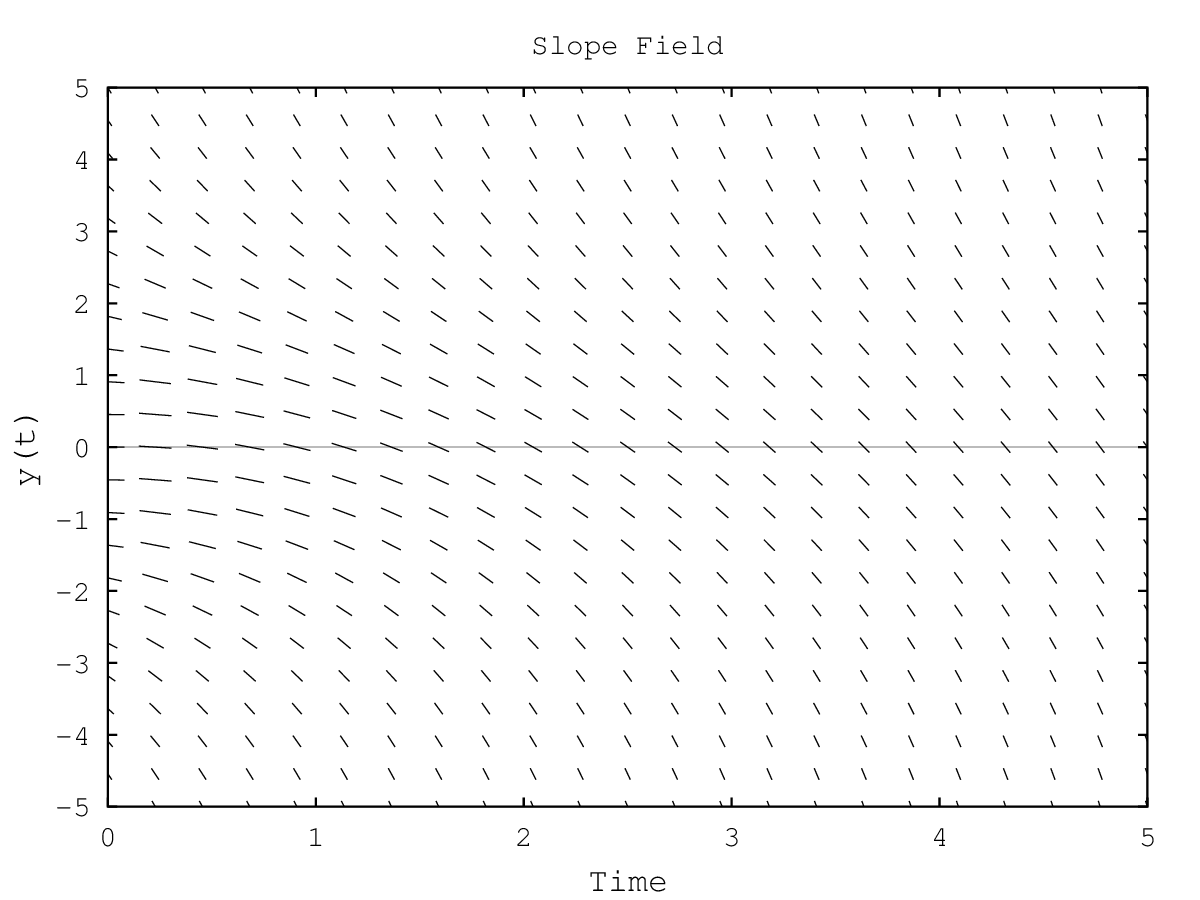
\includegraphics[height=5cm]{img/stabilityClicker1}

          \column{.4\textwidth}
          True or False: The solution to this differential equation is stable.

          \begin{tabular}{l@{\hspace{3em}}l}
            A: & True. \\
            B: & False. \\
            C: & Who knows? \\
            D: & Truth is subjective. \\ 
          \end{tabular}

        \end{columns}

     }\fi

     \ifnum\value{clickerQuiz}=2{%

        Look at the slope field:
        \begin{eqnarray*}
          y' & = & \frac{3}{2}-y?
        \end{eqnarray*}


        \begin{columns}
          \column{.6\textwidth} 

          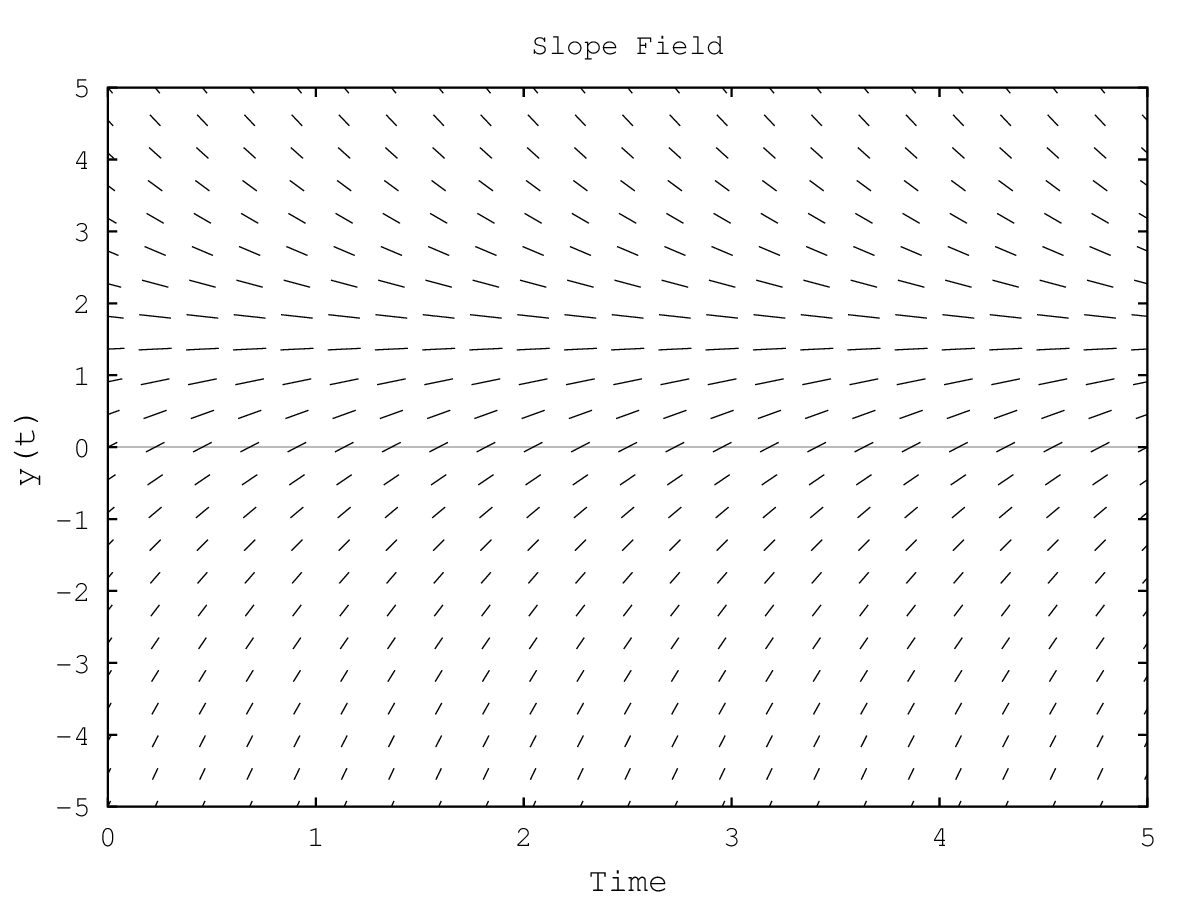
\includegraphics[height=5cm]{img/stabilityClicker2}

          \column{.4\textwidth}
          True or False: The solution to this differential equation is stable.

          \begin{tabular}{l@{\hspace{3em}}l}
            A: & True. \\
            B: & False. \\
            C: & Who knows? \\
            D: & Truth is subjective. \\ 
          \end{tabular}

        \end{columns}

     }\fi

      \ifnum\value{clickerQuiz}=3{%
      Look at the slope field:
        \begin{eqnarray*}
          x' & = & x^2-4?
        \end{eqnarray*}


        \begin{columns}
          \column{.6\textwidth}

          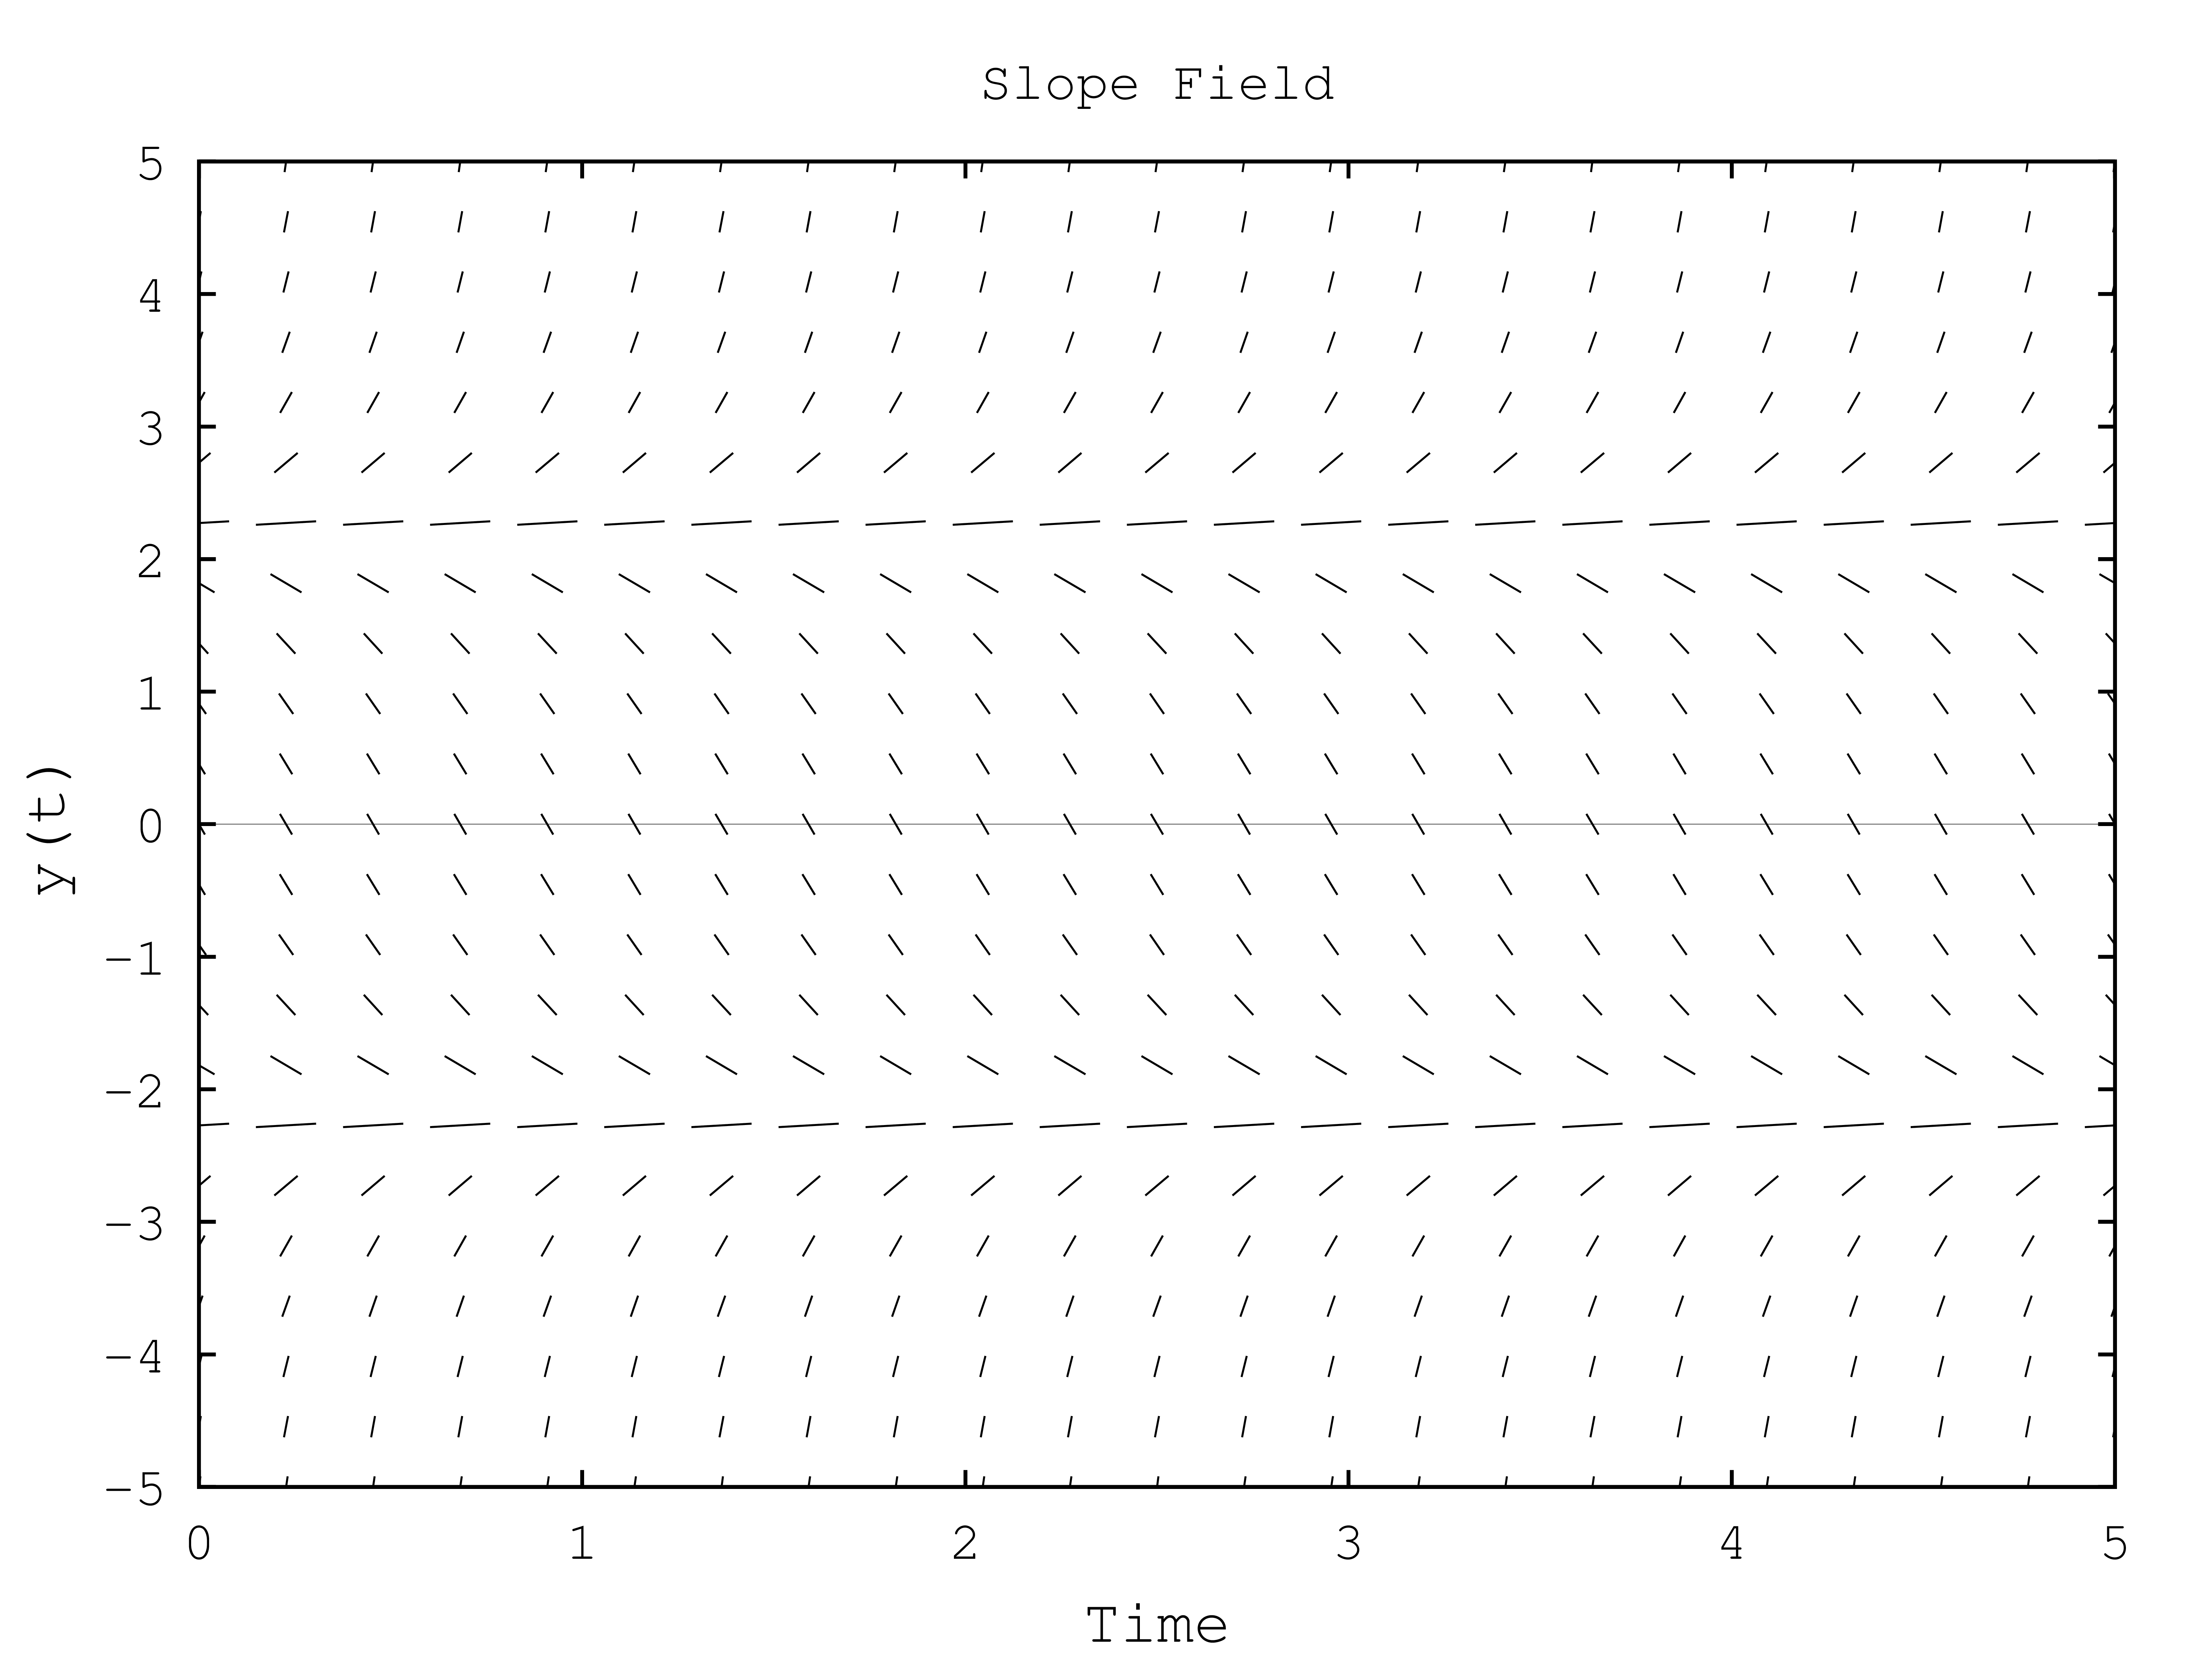
\includegraphics[height=5cm]{img/slopefield2}

          \column{.4\textwidth}
          True or False: The solution to this differential equation is stable.

          \begin{tabular}{l@{\hspace{1em}}l}
            A: & True. \\
            B: & False. \\
            C: & Who knows? \\
            D: & Truth is subjective. \\
          \end{tabular}

        \end{columns}

     }\fi

    \vfill
    \vfill
    \vfill

\end{frame}

}


\subsection{Autonomous DEs}

\begin{frame}
  \frametitle{Autonomous DEs}

  A differential equation is \textit{autonomous} if it can be
  expressed in the form
  \begin{eqnarray*}
    y' & = & f(y).
  \end{eqnarray*}

  i.e. the DE does not have a time term explicitly given in the
  equation.


\end{frame}


\begin{frame}
  \frametitle{The slope only depends on y!}

  \vspace*{-3em}
  \begin{eqnarray*}
    y' & = & f(y).
  \end{eqnarray*}

  If the slope at $y=1$ and $t=1$ is $\half$, then it will be the same
  slope for all points where $y=1$. 

  \vfill
  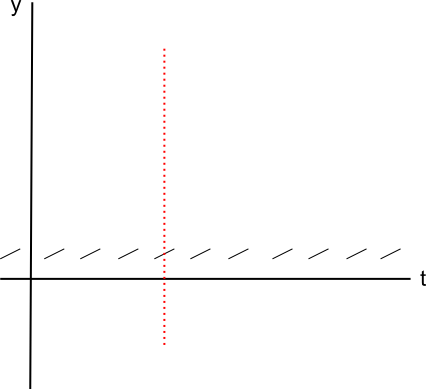
\includegraphics[width=5cm]{img/autonomousEqnSlopeField}
  \vfill

  We just need to find the slope for each value of $y$ and not worry
  about $t$.

\end{frame}

\begin{frame}
  \frametitle{The Phase Line}

  The phase line for a differential equation is a vertical line that
  indicates whether the slope is positive, negative, or zero for
  different values of $y$.
\end{frame}

\begin{frame}
  \frametitle{Example}
  \begin{eqnarray*}
    y' & = & 2y(3-y), \\
    \Rightarrow f(y) & = & 2y(3-y)
  \end{eqnarray*}


  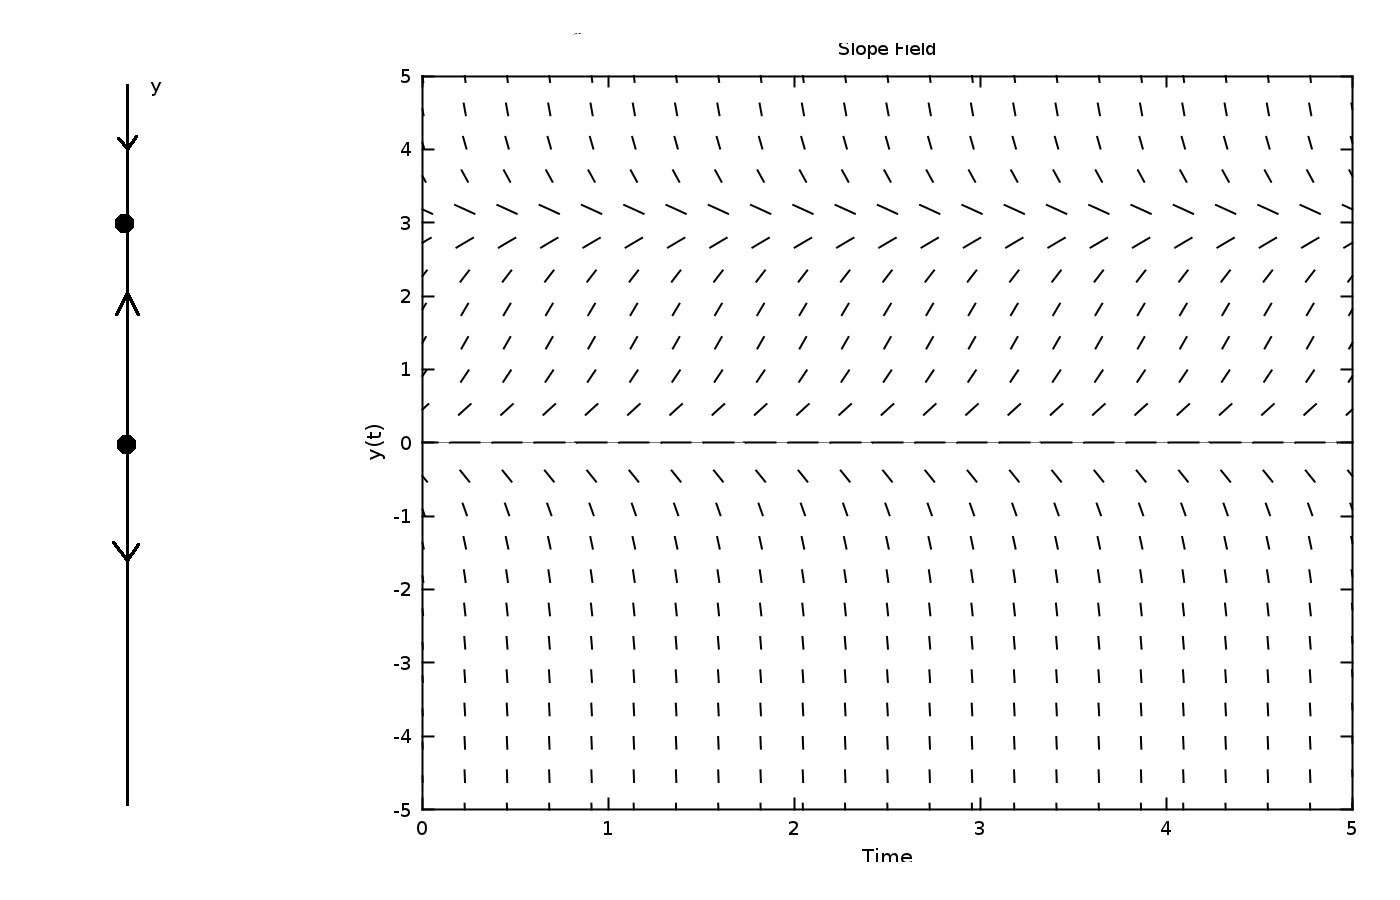
\includegraphics[height=6cm]{img/week3PhaseLineExample1}

\end{frame}


\begin{frame}
  \frametitle{Examples}
  
  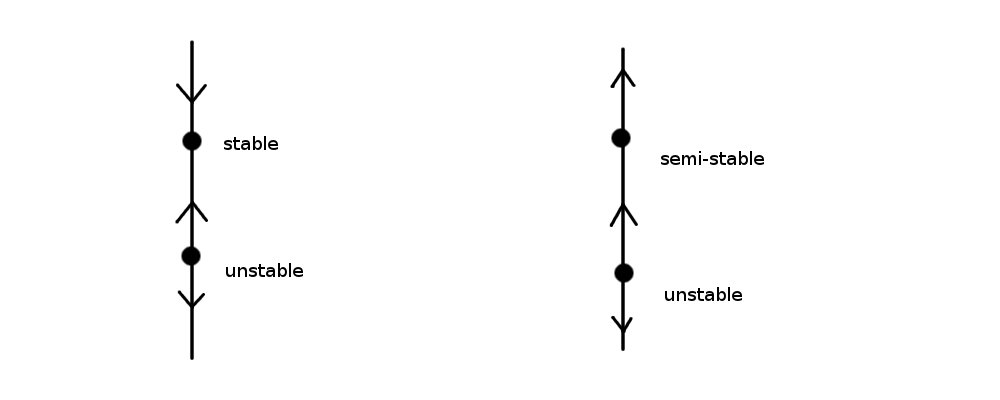
\includegraphics[height=6cm]{img/week3PhaseLine}

\end{frame}

\begin{frame}
  \frametitle{Examples}


  \begin{eqnarray*}
    y' & = & y(2-y)(4-y), \\
    \Rightarrow f(y) & = & y(2-y)(4-y)
  \end{eqnarray*}

  \begin{eqnarray*}
    y' & = & y(2-y^2), \\
    \Rightarrow f(y) & = & y(2-y^2)
  \end{eqnarray*}

  (phase lines drawn on board)

\end{frame}

\iftoggle{clicker}{%
\begin{frame}
  \frametitle{Clicker Quiz}
    
      \ifnum\value{clickerQuiz}=1{%

        Which phase line is the correct phase line for the
        differential equation
        \begin{eqnarray*}
          y ' & = & y^3-y^2
        \end{eqnarray*}

          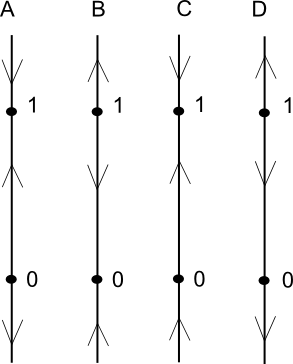
\includegraphics[height=5cm]{img/phaseLinesClickerSect1}

     }\fi

     \ifnum\value{clickerQuiz}=2{%


        Which phase line is the correct phase line for the
        differential equation
        \begin{eqnarray*}
          y ' & = & y^2 + 3y - 4
        \end{eqnarray*}

        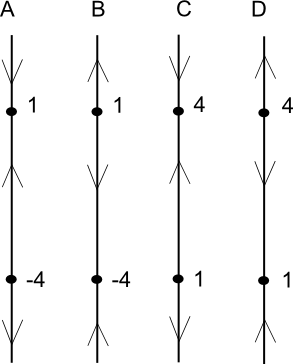
\includegraphics[height=5cm]{img/phaseLinesClickerSect2}


     }\fi

      \ifnum\value{clickerQuiz}=3{%
       Which phase line is the correct phase line for the
        differential equation
        \begin{eqnarray*}
          y ' & = & y^3-y^2
        \end{eqnarray*}

          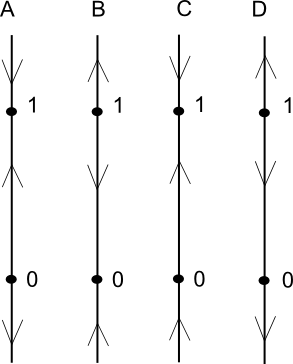
\includegraphics[height=5cm]{img/phaseLinesClickerSect1}
     }\fi

    \vfill
    \vfill
    \vfill

\end{frame}

}



\subsection{Logistic Growth}

\begin{frame}
  \frametitle{Logistic Growth}

  \vspace*{-4em}
  \begin{eqnarray*}
    y' & = & ky,
  \end{eqnarray*}
  
  If $y$ is ``small'' $k$ should be positive.

  If $y$ is ``big'' $k$ should be negative.

  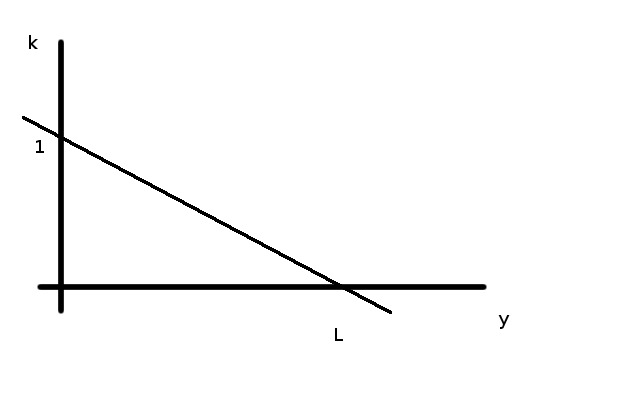
\includegraphics[height=4cm]{img/week3GrowthRate}

  Let 
  \begin{eqnarray*}
    k & = & r \lp 1 - \frac{y}{L} \rp
  \end{eqnarray*}


\end{frame}


\begin{frame}
  \frametitle{Logistic Equation}

  \begin{eqnarray*}
    y' & = & r \lp 1 - \frac{y}{L} \rp y
  \end{eqnarray*}

  Stationary points: $y=0$ and $y=L$. 

  ($L$ is called the ``carrying capacity'')

  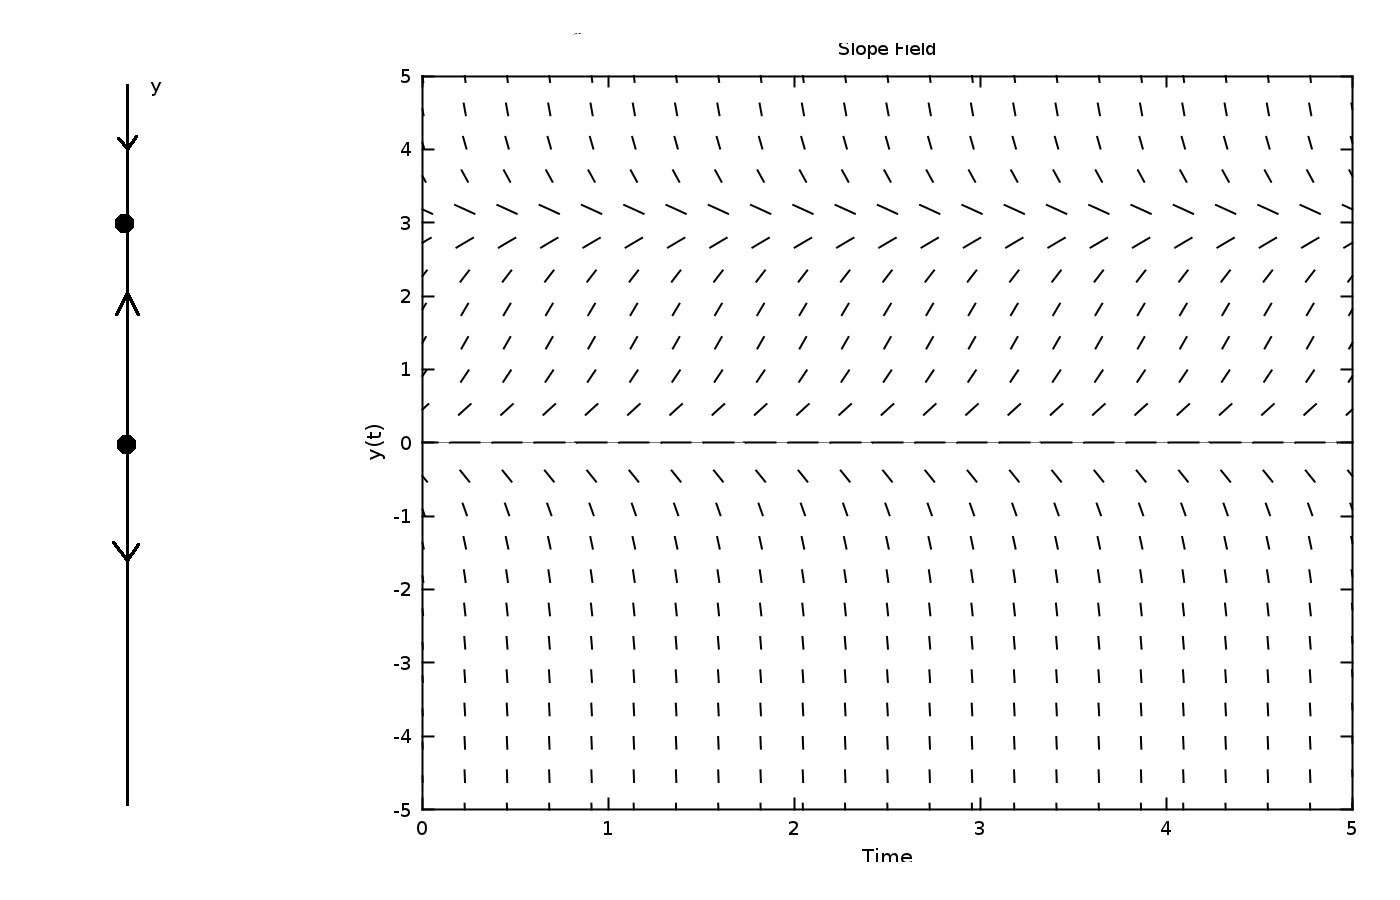
\includegraphics[height=6cm]{img/week3PhaseLineExample1}

\end{frame}


\begin{frame}
  \frametitle{Analytic Solution}

  \begin{eqnarray*}
    y' & = & r \lp 1 - \frac{y}{L} \rp y, \\
    \uncover<2->{
      \frac{y'}{\lp 1 - \frac{y}{L} \rp y} & = & r \\
      \int \frac{y'}{\lp 1 - \frac{y}{L} \rp y} ~ dt & = & \int r ~ dt       
    }
  \end{eqnarray*}

\end{frame}


\begin{frame}


  \begin{eqnarray*}
    \frac{1}{\lp 1 - \frac{y}{L} \rp y} & = & \frac{a}{1 - \frac{y}{L}} + \frac{b}{y} \\
    \Rightarrow 1 & = & a y + b \lp 1 - \frac{y}{L} \rp \\
    b & = & 1, \\
    a & = & \frac{1}{L}
  \end{eqnarray*}

    
\end{frame}

  \begin{frame}

  \begin{eqnarray*}
      \int \frac{1}{\lp 1 - \frac{y}{L} \rp y} ~ dy & = & \int r ~ dt \\
      \int \frac{1}{L} \cdot \frac{1}{1 - \frac{y}{L}} + \frac{1}{y} ~ dy & = & \int r ~ dt \\
      -\ln\lp 1 - \frac{y}{L}\rp + \ln(y) & = & rt + C \\
      \ln\lp\frac{y}{1 - \frac{y}{L}}\rp & = & rt + C \\
      \frac{y}{1 - \frac{y}{L}} & = & k e^{rt} \\
      \Rightarrow y & = & \frac{k e^{rt}}{1 + \frac{1}{L} k e^{rt}}  
  \end{eqnarray*}


  From the initial condition,
  \begin{eqnarray*}
    y(0) & = & y_0, \\
    k & = & \frac{y_0}{1 - \frac{y_0}{L}}
  \end{eqnarray*}
  

\end{frame}



% LocalWords:  Clarkson pausesection hideothersubsections




% %%%%%%%%%%%%%%%%%%%%%%%%%%%%%%%%%%%%%%%%%%%%%%%%%%%%%%%%%%%%

\include{week4-Day1}

\part{Complex-Numbers-II}
\lecture{Complex Numbers II}{Complex-Numbers-II}
\section{Complex Numbers II}

\title{Ordinary Differential Equations}
\subtitle{Math 232 - Week 5, Day 1}
\date{26 Sep 2012}

\begin{frame}
  \titlepage
\end{frame}

\begin{frame}
  \frametitle{Outline}
  \tableofcontents[pausesection,hideothersubsections]
\end{frame}


\subsection{Root Finding}


\begin{frame}
  \frametitle{Example}

  Find the cubic roots of $2+2i$.

  \begin{eqnarray*}
    2 + 2i & = & 2\sqrt{2} e^{i\pi/4}
  \end{eqnarray*}

  Let $z=re^{i\theta}$ so $z^3=r^3e^{i3\theta}$:
  \begin{eqnarray*}
    r^3e^{i3\theta} & = & 2\sqrt{2} e^{i\pi/4}, ~ 2\sqrt{2} e^{i9\pi/4}, ~ 2\sqrt{2} e^{i17\pi/4}
  \end{eqnarray*}

  \begin{eqnarray*}
    r &  = & (2\sqrt{2})^{1/3} \\
    \theta & = & \frac{\pi}{12}, ~ \frac{9\pi}{12}, ~ \frac{17\pi}{12} \\
    z & = &  (2\sqrt{2})^{1/3} e^{i\pi/12}, ~ (2\sqrt{2})^{1/3} e^{i9\pi/12}, ~ (2\sqrt{2})^{1/3} e^{i17\pi/12}
  \end{eqnarray*}

\end{frame}


\begin{frame}
  \frametitle{Example}

  Find the square roots of $\sqrt{3}+i$

  \begin{eqnarray*}
    \sqrt{3} + i & = & 2 e^{\pi/6} 
  \end{eqnarray*}

  Let $z=re^{i\theta}$ so $z^2=r^2e^{i2\theta}$:
  \begin{eqnarray*}
    r^2e^{i2\theta} & = & 2 e^{\pi/6} , ~ 2 e^{13\pi/6} 
  \end{eqnarray*}

  \begin{eqnarray*}
    r & = & \sqrt{2} \\
    \theta & = & \frac{\pi}{12}, ~ \frac{13\pi}{12}
  \end{eqnarray*}

\end{frame}


\begin{frame}
  \frametitle{Important Properties}

  Euler's Formula
  \begin{eqnarray*}
    e^{it} & = & \cos(t) + i\sin(t). 
  \end{eqnarray*}

  Note:
  \begin{eqnarray*}
    e^{-it} & = & \cos(-t) + i\sin(-t) \\
    & = & \cos(t) - i\sin(t)
  \end{eqnarray*}

  So...
  \begin{eqnarray*}
    e^{it} + e^{-it} & = & 2 \cos(t), \\
    \frac{e^{it} + e^{-it}}{2} & = & \cos(t).
  \end{eqnarray*}

  Also,
  \begin{eqnarray*}
    e^{it} - e^{-it} & = & 2 i \sin(t), \\
    \frac{e^{it} - e^{-it}}{2i} & = & \sin(t).
  \end{eqnarray*}



\end{frame}


\begin{frame}
  \frametitle{Quick Example}

  \begin{eqnarray*}
    \cos(3t) & = & \frac{e^{i3t}+e^{-i3t}}{2} \\
    \sin(4t) & = & \frac{e^{i4t}-e^{-i4t}}{2i}
  \end{eqnarray*}

\end{frame}


\begin{frame}
  \frametitle{Another thing...}

  \begin{eqnarray*}
    e^{a+ib} & = & e^a e^{ib} \\
    & = & e^a \lp \cos(b) + i \sin(b) \rp.
  \end{eqnarray*}

  Thusly...
  \begin{eqnarray*}
    e^{a-ib} & = & e^a \lp \cos(b) - i \sin(b) \rp.
  \end{eqnarray*}

\end{frame}


\begin{frame}
  \frametitle{What do we have here?}

  \begin{eqnarray*}
    e^a \cos(b) & = & e^a \lp \frac{e^{ib}+e^{-ib}}{2} \rp \\
    & = & \half e^a e^{ib} +\half e^a  e^{-ib} \\
    e^a \sin(b) & = & e^a \lp \frac{e^{ib}-e^{-ib}}{2i} \rp \\
    & = & \frac{1}{2i} e^a e^{ib} - \frac{1}{2i} e^a e^{-ib}
  \end{eqnarray*}

\end{frame}

\subsection{Derivatives and Integrals}

\begin{frame}
  \frametitle{Derivatives and Integrals}

  \begin{eqnarray*}
    f(t) & = & u(t) + i v(t) \\
    f'(t) & = & u'(t) + i v'(t),
  \end{eqnarray*}

  and
  \begin{eqnarray*}
    \int f(t) ~ dt & = & \int u(t) + i v(t) ~ dt, \\
    & = & \int u(t) ~ dt + i \int v(t) ~ dt.
  \end{eqnarray*}

\end{frame}


\begin{frame}
  \frametitle{Examples}

  \begin{eqnarray*}
    \frac{d}{dt} \lp \sin(t) + i e^{2t} \cos(t) \rp & = & 
    \cos(t) + i \lp 2 e^{2t} \cos(t) - e^{2t} \sin(t) \rp.
  \end{eqnarray*}

  \begin{eqnarray*}
    \int \sin(t) + i t \cos(t) ~ dt & = & 
    \int \sin(t) ~ dt + i \int t \cos(t) ~ dt \\
    \cos(t) + i \lp t\sin(t) + \cos(t) \rp + C
  \end{eqnarray*}

  Note that ``$C$'' is a complex number!
  \begin{eqnarray*}
    C & = & C_1 + i C_2.
  \end{eqnarray*}

\end{frame}

\subsection{What does this have to do with DEs?}

\begin{frame}
  \frametitle{Why do we care?}

  Show that $y=C_1 e^{(-3+i)t} + C_2 e^{(-3-)t}$ is a solution to the DE
  \begin{eqnarray*}
    y'' + 6y' + 10y & = & 0.
  \end{eqnarray*}

\end{frame}




% LocalWords:  Clarkson pausesection hideothersubsections



% %%%%%%%%%%%%%%%%%%%%%%%%%%%%%%%%%%%%%%%%%%%%%%%%%%%%%%%%%%%%



\newcommand{\arrayTwo}[4]{
  \left[
  \begin{array}{rr}
    #1 & #2 \\
    #3 & #4
  \end{array}
  \right]
}

\newcommand{\vecTwo}[2]{
  \left[
  \begin{array}{r}
    #1 \\  #2
  \end{array}
  \right]
}


\newcommand{\stateTwo}[2]{
  \begin{array}{rr}
    \mbox{\fontsize{6}{6}\selectfont $#1$} \\  \mbox{\fontsize{6}{6}\selectfont $#2$}
  \end{array}
}


\newcommand{\arrayThree}[9]{
  \left[
    \begin{array}{rrr}
      #1 & #2 & #3 \\
      #4 & #5 & #6 \\
      #7 & #8 & #9
    \end{array}
  \right]
}

\newcommand{\startRowOps}{
  \left[
    \begin{array}{rrr|r}
}

\newcommand{\oneRowOps}[4] {
      #1 & #2 & #3 & #4 \\
}

\newcommand{\stopRowOps}{
    \end{array}
  \right]
}


\newcommand{\vecThree}[3]{
  \left[
  \begin{array}{r}
    #1 \\  #2 \\ #3
  \end{array}
  \right]
}


\newcommand{\stateThree}[3]{
  \begin{array}{r}
    \mbox{\fontsize{6}{6}\selectfont $#1$} \\  
    \mbox{\fontsize{6}{6}\selectfont $#2$} \\ 
    \mbox{\fontsize{6}{6}\selectfont $#3$}
  \end{array}
}





\newcommand{\detTwo}[4]{
  \left|
  \begin{array}{rr}
    #1 & #2 \\
    #3 & #4
  \end{array}
  \right|
}



\newcommand{\detThree}[9]{
  \left|
    \begin{array}{rrr}
      #1 & #2 & #3 \\
      #4 & #5 & #6 \\
      #7 & #8 & #9
    \end{array}
  \right|
}




\newcommand{\startRowFour}{
  \left[
    \begin{array}{rrrr}
}

\newcommand{\oneRowFour}[4] {
      #1 & #2 & #3 & #4 \\
}




\documentclass{beamer}

\mode<presentation>





\usetheme{Frankfurt}%
\usecolortheme{seagull}
\logo{
\includegraphics[height=.25in]{clarksonGreen}}

\definecolor{garnet}{RGB}{136,0,0}
%\definecolor{clarksonGreen}{RGB}{0,71,28}
\definecolor{clarksonGreen}{RGB}{0,52,21}
\setbeamercolor{palette primary}{fg=clarksonGreen,bg=white}
\setbeamercolor{palette secondary}{fg=clarksonGreen,bg=white}
\setbeamercolor{palette tertiary}{fg=clarksonGreen,bg=white}
\setbeamercolor{palette quaternary}{bg=clarksonGreen,fg=white}
\setbeamercolor{block title}{fg=black,bg=black!15}
\setbeamercolor{block body}{fg=black,bg=black!10}
\setbeamercolor{titlelike}{bg=clarksonGreen,fg=white} % parent=palette quaternary}

\newcommand{\half}{\mbox{$\frac{1}{2}$}}
\newcommand{\deltat}{\mbox{$\triangle t$}}
\newcommand{\deltax}{\mbox{$\triangle x$}}
\newcommand{\deltay}{\mbox{$\triangle y$}}

\newcommand{\deriv}[2]{\frac{d}{d#2}#1}
\newcommand{\derivTwo}[2]{\frac{d^2}{d#2^2}#1}

\newcommand{\lp}{\left(}
\newcommand{\rp}{\right)}


\newcommand{\arrayTwo}[4]{
  \left[
  \begin{array}{rr}
    #1 & #2 \\
    #3 & #4
  \end{array}
  \right]
}

\newcommand{\vecTwo}[2]{
  \left[
  \begin{array}{rr}
    #1 \\  #2
  \end{array}
  \right]
}




\begin{document}

\title{Ordinary Differential Equations}
\subtitle{Math 232 - Week 5, Day 2}

\author{Kelly Black}
\institute{Clarkson University}
\date{28 Sep 2011}

\begin{frame}
  \titlepage
\end{frame}

\begin{frame}
  \frametitle{Outline}
  \tableofcontents[pausesection,hideallsubsections]
\end{frame}


\section{Linear Algebra}


\begin{frame}
  \frametitle{Linear Algebra}


  \begin{eqnarray*}
    3x + 2y & = & 7 \\
    4x - y & = & 1
  \end{eqnarray*}

  \uncover<2->
  {
    \begin{eqnarray*}
      \arrayTwo{3}{2}{4}{-1} \vecTwo{x}{y} & = & \vecTwo{7}{1}
    \end{eqnarray*}

    A matrix is an array of numbers arranged in rows and columns.

    A column vector is a matrix with one column.

  }


\end{frame}


\begin{frame}
  \frametitle{Matrix Addition/Subtraction}

  If two matrices have the same number of rows and columns you add the
  two matrices by adding/subtracting them entry by entry.

  \begin{eqnarray*}
    \arrayTwo{3}{-1}{2}{4} + \arrayTwo{7}{6}{2}{1} & = & \arrayTwo{10}{5}{4}{5}
  \end{eqnarray*}

\end{frame}


\begin{frame}
  \frametitle{Scalar Multiplication}

  Multiply every entry in the matrix by the same number.

  \begin{eqnarray*}
    4 \arrayTwo{3}{-1}{2}{4} & = & \arrayTwo{12}{-4}{8}{16}
  \end{eqnarray*}


\end{frame}


\begin{frame}
  \frametitle{Transpose}

  Switch the rows and the columns:
  \begin{eqnarray*}
    \arrayTwo{2}{7}{4}{6}^T & = & \arrayTwo{2}{4}{7}{6} \\
    \left[
    \begin{array}{r}
      1 \\ 7 \\ 3 \\ 2
    \end{array}
    \right]^T & = & 
    \left[
    \begin{array}{rrrr}
      1 & 7 & 3 & 2
    \end{array}
    \right]
  \end{eqnarray*}

\end{frame}


\begin{frame}
  \frametitle{Matrix Multiplication}

  \begin{eqnarray*}
    \left[
    \begin{array}{rrrr}
      a_{11} & a_{12} & \cdots & a_{1m} \\
      a_{21} & a_{22} & \cdots & a_{2m} \\
      \vdots &       & \ddots & \vdots \\ \hline
      a_{i1} & a_{i2} & \cdots & a_{im} \\ \hline
      \vdots &       & \ddots & \vdots \\
      a_{n1} & a_{n2} & \cdots & a_{nm}
    \end{array}
  \right] \cdot
    \left[
    \begin{array}{rr|r|rr}
      b_{11} & \cdots & b_{1j} & \cdots  & b_{1k} \\
      b_{21} & \cdots & b_{2j} & \cdots  & b_{2k} \\
      \vdots &        & \vdots & \vdots & \vdots \\
      b_{n1} & \cdots & b_{mj}  & \cdots & b_{mk}
    \end{array}
  \right]  =  \\
    \left[
    \begin{array}{rrrrr}
      * & \cdots & * & \cdots  &  * \\
      *  & \cdots & *  & \cdots  &  * \\
      \vdots &        & c_{ij} & \vdots & \vdots \\
      * & \cdots & *  & \cdots & *
    \end{array}
  \right]
  \end{eqnarray*}

  Entry in row i and column j is 
  \begin{eqnarray*}
    c_{ij} & = & a_{i1}b_{1j} + a_{i2}b_{2j} + \cdots + a_{im}b_{mj}
  \end{eqnarray*}

\end{frame}


\begin{frame}
  \frametitle{Example}

  \begin{eqnarray*}
    \arrayTwo{2}{7}{4}{6} \cdot \arrayTwo{2}{1}{-2}{1} & = & 
    \arrayTwo{-10}{9}{-4}{10} \\
    \left[
      \begin{array}{rrr}
        2 & 3 & 1 \\ -1 & 2 & 1
      \end{array}
    \right] \cdot
    \left[
      \begin{array}{r}
        1 \\ 2 \\ 3
      \end{array}
    \right]
    & = & 
    \vecTwo{11}{6}
  \end{eqnarray*}

\end{frame}

\section{Vector Operations}

\begin{frame}
  \frametitle{Vector Operations}

  If
  \begin{eqnarray*}
    \vec{x} & = & 
    \left[
    \begin{array}{r}
      x_1 \\ x_2 \\ \vdots \\ x_n
    \end{array}
    \right]
  \end{eqnarray*}
  then
  \begin{eqnarray*}
    \left[
      \begin{array}{rrrr}
        x_1 & x_2 & \cdot & x_n
      \end{array}
    \right] \cdot
    \left[
      \begin{array}{r}
        x_1 \\ x_2 \\ \vdots \\ x_n
      \end{array}
    \right] & = & 
    x_1^2 + x_2^2 + \cdots x_n^2
  \end{eqnarray*}

\end{frame}


\begin{frame}
  \frametitle{The Dot Product}

  Definition:
  \begin{eqnarray*}
    \vec{x} \cdot \vec{y} & = & \vec{x}^T \vec{y} 
  \end{eqnarray*}

  Definition
  \begin{eqnarray*}
    \| \vec{x} \| & = & \sqrt{\vec{x}^T \vec{x}}
  \end{eqnarray*}

\end{frame}


\begin{frame}
  \frametitle{Example}

  \begin{eqnarray*}
    \vec{x} & = & 
    \left[
      \begin{array}{r}
        2 \\ 4 \\ -1
      \end{array} \right] \\
      \| \vec{x} \| & = & \sqrt{2^2 + 4^2 + (-1)^2} \\
      & = & \sqrt{21}
  \end{eqnarray*}

\end{frame}

\section{Matrices to Know}

\begin{frame}
  \frametitle{Matrices to Know}
  
  A diagonal matrix is in the form
  \begin{eqnarray*}
    \left[
      \begin{array}{rrrr}
        a_{11} & 0 & \\
        0 & a_{22} & 0 \\
        & & \ddots & \\
        & & 0 & a_{nn}
      \end{array}
    \right]
  \end{eqnarray*}

  Special case, the identity matrix:
  \begin{eqnarray*}
    I_n & = & 
    \left[
      \begin{array}{rrrr}
        1 & 0 & \\
        0 & 1 & 0 \\
        & & \ddots & \\
        & & 0 & 1
      \end{array}
    \right]
  \end{eqnarray*}

\end{frame}


\begin{frame}
  \frametitle{Example}
  
  Special case, the identity matrix:
  \begin{eqnarray*}
    I_3 & = & 
    \left[
      \begin{array}{rrr}
        1 & 0 & 0\\
        0 & 1 & 0 \\
        0 & 0 & 1
      \end{array}
    \right]
  \end{eqnarray*}

  Note:
  \begin{eqnarray*}
    \left[
      \begin{array}{rrr}
        1 & 0 & 0 \\
        0 & 1 & 0 \\
        0 & 0 & 1
      \end{array}
    \right] \cdot
       \left[
      \begin{array}{rrr}
        3 & 4 & 2 \\
        -5 & 6 & 7 \\
        8 & 7 & 3
      \end{array}
    \right] & = & 
       \left[
      \begin{array}{rrr}
        3 & 4 & 2 \\
        -5 & 6 & 7 \\
        8 & 7 & 3
      \end{array}
    \right] 
  \end{eqnarray*}

  In general $I_n\cdot A = A$.

\end{frame}

\section{Orthogonality}

\begin{frame}
  \frametitle{Orthogonality}

  \begin{eqnarray*}
    \vec{x} & = & \vecTwo{1}{0} \\
    \vec{y} & = & \vecTwo{0}{1} \\
    \vec{x}\cdot\vec{y} & = & 0
  \end{eqnarray*}

  In general,
  \begin{eqnarray*}
    \vec{u}\cdot\vec{v} & = & \| \vec{u} \| \| \vec{v} \| \cos(\theta)
  \end{eqnarray*}

  Definition, if $\vec{u}\cdot\vec{v}=0$ then the vectors are \textbf{orthogonal}.
  
\end{frame}

\section{Differentiation}

\begin{frame}
  \frametitle{Differentiation}

  The derivative of a matrix is the derivative of each of its elements.
  \begin{eqnarray*}
    \frac{d}{dt} \arrayTwo{3t^{-1}}{\sin(t)}{\sqrt{t+1}}{\tan(t)} & = & 
    \arrayTwo{-3t^{-2}}{\cos(t)}{\half\lp t+1\rp^{-\half}}{\sec^2(t)}
  \end{eqnarray*}

\end{frame}

\begin{frame}
  \frametitle{Why bother?}

  Suppose that
  \begin{eqnarray*}
    \frac{d}{dt} x & = & 3x + 2y \\
    \frac{d}{dt} y & = & -2 x + 4 y
  \end{eqnarray*}

  Another way to express the system:
  \begin{eqnarray*}
    \frac{d}{dt} \vecTwo{x}{y} & = & \arrayTwo{3}{2}{-2}{4} \vecTwo{x}{y}
  \end{eqnarray*}

\end{frame}

\end{document}

% LocalWords:  Clarkson pausesection hideallsubsections


\part{Linear-Systems}
\lecture{Linear Systems}{Linear-Systems}
\section{Linear Systems}

\title{Ordinary Differential Equations}
\subtitle{Math 232 - Week 5, Day 2}
\date{26 Sep 2012}

\begin{frame}
  \titlepage
\end{frame}

\begin{frame}
  \frametitle{Outline}
  \tableofcontents[pausesection,hideothersubsections]
\end{frame}


\subsection{Linear Systems}


\begin{frame}
  \frametitle{What is a solution to a linear system?}

  \begin{eqnarray*}
    3x + y & = & 4 \\
    -2x + y & = & 2
  \end{eqnarray*}

  What is the value of $x$ and $y$?

  \uncover<2->{How to solve?}
  \begin{itemize}
  \item<3-> Solve for $x$, substitute into the second equation, solve
    for $y$, and then substitute that result back in to the first
    equation.
  \item<4-> What if you have hundreds of equations and hundreds of
    unknowns?
  \item<5-> We need a better way!
  \end{itemize}

\end{frame}


\begin{frame}
  \frametitle{Canceling variables in a clever way}

  \begin{eqnarray*}
    3x + y & = & 4 \\
    -2x + y & = & 2 \\
    \\
    \Rightarrow
    x + \frac{1}{3}y & = & \frac{4}{3} \\
    -2x + y & = & 2 \\    
  \end{eqnarray*}
  
  Now take 2*(Equation 1) + (Equation 2).

\end{frame}


\begin{frame}
  \frametitle{Canceling variables in a clever way}

  \begin{eqnarray*}
    x + \frac{1}{3}y & = & \frac{4}{3} \\
    \frac{5}{3}  y & = & \frac{14}{3} \\
  \end{eqnarray*}

  Solving for $y$ first we get
  \begin{eqnarray*}
    y & = & \frac{14}{5}.
  \end{eqnarray*}

  Now substitute back into the first equation to get
  \begin{eqnarray*}
    x & = & \frac{4}{3} - \frac{1}{3} y \\
    & = & \frac{2}{5}
  \end{eqnarray*}

  The two lines meet at the point $x=\frac{2}{5}$ and $y=\frac{14}{5}$.

\end{frame}

\subsection{Solving in Matrix Notation}

\begin{frame}
  \frametitle{Using Matrix Notation}

  \begin{eqnarray*}
    \arrayTwo{3}{1}{-2}{1} \vecTwo{x}{y} & = & \vecTwo{4}{2} \\
    \uncover<2->{
      \Rightarrow
      \stateTwo{R_1/3}{~}
      \arrayTwo{1}{\frac{1}{3}}{-2}{1} \vecTwo{x}{y} & = & \vecTwo{\frac{4}{3}}{2} \\
    }
    \uncover<3->{
      \Rightarrow
      \stateTwo{~}{2R_1+R2}
      \arrayTwo{1}{\frac{1}{3}}{0}{\frac{5}{3}} \vecTwo{x}{y} & = & \vecTwo{\frac{4}{3}}{\frac{14}{3}}
    }
  \end{eqnarray*}
  \uncover<4->{Exactly the same thing only I am using matrices to
    track the coefficients.}

\end{frame}


\begin{frame}
  \frametitle{Example}

  \begin{eqnarray*}
    2x + 4y - z & = & 6 \\
    x + y + z & = & 2 \\
    -3x + y + 2z & = & 7 \\
    \\
    \uncover<2->
    {
      \arrayThree{2}{4}{-1}{1}{1}{1}{-3}{1}{2}
      \vecThree{x}{y}{z}
      & = & 
      \vecThree{6}{2}{7}
    } 
  \end{eqnarray*}

\end{frame}


\begin{frame}

  \begin{eqnarray*}
    \stateThree{R_1/2}{~}{~}
    \arrayThree{1}{2}{-0.5}{1}{1}{1}{-3}{1}{2} \vecThree{x}{y}{z} & = & \vecThree{3}{2}{7} \\
    \uncover<2->
    {
      \stateThree{~}{-R_1+R_2}{3R_1+R_3}
      \arrayThree{1}{2}{-0.5}{0}{-1}{1.5}{0}{7}{0.5} \vecThree{x}{y}{z} & = & \vecThree{3}{-1}{16} \\ 
    }
    \uncover<3->
    {
      \stateThree{~}{-R_2}{~}
      \arrayThree{1}{2}{-0.5}{0}{1}{-1.5}{0}{7}{0.5} \vecThree{x}{y}{z} & = & \vecThree{3}{1}{16} \\ 
    }
    \uncover<4->
    {
      \stateThree{~}{~}{-7R_2+R_3}
      \arrayThree{1}{2}{-0.5}{0}{1}{-1.5}{0}{0}{11} \vecThree{x}{y}{z} & = & \vecThree{3}{1}{9} 
    }
  \end{eqnarray*}

\end{frame}


\begin{frame}
  \frametitle{Note}

  \begin{eqnarray*}
    \stateThree{~}{~}{R_3/11}
    \arrayThree{1}{2}{-0.5}{0}{1}{-1.5}{0}{0}{1} \vecThree{x}{y}{z} & = & \vecThree{3}{1}{9/11} \\
    \uncover<2->
    {
      \stateThree{R_1+ 1/2 R_3}{R_2 + 3/2 R_3}{~}
      \arrayThree{1}{2}{0}{0}{1}{0}{0}{0}{1} \vecThree{x}{y}{z} & = & \vecThree{75/22}{49/22}{9/11} \\
    }
    \uncover<3->
    {
      \stateThree{R_1-2R_2}{~}{~}
      \arrayThree{1}{0}{0}{0}{1}{0}{0}{0}{1} \vecThree{x}{y}{z} & = & \vecThree{-23/22}{49/22}{9/11}
    }
  \end{eqnarray*}
  \uncover<4->{``Reduced Row Echelon'' See definition at the top of page 136.}

\end{frame}

\subsection{More Compact Notation}

\begin{frame}
  \frametitle{Example}

  \begin{eqnarray*}
    2x + 4y + 6z & = & 8 \\
    x - y + z & = & 4 \\
    4x + 2y + 8z & = & 4 \\
    ~ \\
    \uncover<2->
    {
      \stateThree{~}{~}{~}
      \startRowOps
      \oneRowOps{2}{4}{6}{8} 
      \oneRowOps{1}{-1}{1}{4} 
      \oneRowOps{4}{2}{8}{4} 
      \stopRowOps
    }
    \\
    \uncover<3->
    {
      \stateThree{R_1/2}{~}{~}
      \startRowOps
      \oneRowOps{1}{2}{3}{4} 
      \oneRowOps{1}{-1}{1}{4} 
      \oneRowOps{4}{2}{8}{4} 
      \stopRowOps
    }
  \end{eqnarray*}

\end{frame}


\begin{frame}
  \frametitle{Example}

  \begin{eqnarray*}
      \stateThree{~}{-R_1+R_2}{-4R_1+R_3}
      \startRowOps
      \oneRowOps{1}{2}{3}{4} 
      \oneRowOps{0}{-3}{-2}{0} 
      \oneRowOps{0}{-6}{4}{-12} 
      \stopRowOps    \\
      \uncover<2->
      {
        \stateThree{~}{-1/3 R_2}{~}
        \startRowOps
        \oneRowOps{1}{2}{3}{4} 
        \oneRowOps{0}{1}{2/3}{0} 
        \oneRowOps{0}{-6}{4}{-12} 
        \stopRowOps    \\
      }
      \uncover<3->
      {
        \stateThree{~}{~}{6R_2+R_3}
        \startRowOps
        \oneRowOps{1}{2}{3}{4} 
        \oneRowOps{0}{1}{2/3}{0} 
        \oneRowOps{0}{0}{0}{-12} 
        \stopRowOps    
      }
  \end{eqnarray*}

  \uncover<4-> { If one row comes out with zeros except in the last
    column we say that the system is ``not consistent.''}

\end{frame}


\begin{frame}
  \frametitle{Example}
  Suppose instead the system looks like the following:

  \begin{eqnarray*}
    2x + 4y + 6x & = & 8 \\
    x - y + z & = & 4 \\
    4x + 2y + 8z & = & 16 \\
    ~ \\
    \uncover<2->
    {
      \stateThree{~}{~}{~}
      \startRowOps
      \oneRowOps{2}{4}{6}{8} 
      \oneRowOps{1}{-1}{1}{4} 
      \oneRowOps{4}{2}{8}{16} 
      \stopRowOps
    }
    \\
    \uncover<3->
    {
      \stateThree{~}{~}{~}
      \startRowOps
      \oneRowOps{1}{2}{3}{4} 
      \oneRowOps{0}{1}{2/3}{0} 
      \oneRowOps{0}{0}{0}{0} 
      \stopRowOps
    }
  \end{eqnarray*}


  \uncover<4->{If you get all zeros across all of the columns of one
    row so that you have less than ``n'' non-zero rows then the system
    is called ``undetermined.''}

\end{frame}

\begin{frame}
  \frametitle{The RREF of the previous example}

  The RREF of the previous system is the following:
  \begin{eqnarray*}
    \stateThree{~}{~}{~}
    \startRowOps
    \oneRowOps{1}{0}{5/3}{4} 
    \oneRowOps{0}{1}{2/3}{0} 
    \oneRowOps{0}{0}{0}{0} 
    \stopRowOps    
  \end{eqnarray*}

  What does it mean?

  \begin{eqnarray*}
    y + \frac{2}{3}z & = & 0, \\
    \Rightarrow y & = & -\frac{2}{3} z
  \end{eqnarray*}

  \uncover<2->
  {
    \begin{eqnarray*}
      x + \frac{5}{3} z & = & 4, \\
      \Rightarrow x & = & 4 - \frac{5}{3} z
    \end{eqnarray*}
  }

\end{frame}

\begin{frame}
  \frametitle{The Solution}

  \begin{eqnarray*}
    \vecThree{x}{y}{z} & = & \vecThree{4 - \frac{5}{3}z}{-\frac{2}{3}z}{z} \\
    & = & \vecThree{4}{0}{0} + z \vecThree{\frac{-5}{3}}{\frac{-2}{3}}{1}
  \end{eqnarray*}

  For any $z$!
  
\end{frame}

\begin{frame}
  \frametitle{Another Way to Express The Solution}
  
  \begin{eqnarray*}
    \arrayThree{2}{4}{6}{1}{-1}{1}{4}{2}{8} \vecThree{-5/3}{-2/3}{1} 
    & = & \vecThree{0}{0}{0}
  \end{eqnarray*}

  The homogeneous solution is 
  \begin{eqnarray*}
    \vec{x}_h & = & \vecThree{-5/3}{-2/3}{1}. 
  \end{eqnarray*}

\end{frame}

\begin{frame}
  \frametitle{Another Way to Express The Solution}
  
  \begin{eqnarray*}
    \arrayThree{2}{4}{6}{1}{-1}{1}{4}{2}{8} \vecThree{4}{0}{0} 
    & = & \vecThree{8}{4}{16}
  \end{eqnarray*}

  The particular solution is 
  \begin{eqnarray*}
    \vec{x}_p & = & \vecThree{4}{0}{0} 
  \end{eqnarray*}

  \uncover<2->{The solution is
    \begin{eqnarray*}
      \vec{x} & = & \vec{x}_p + C \vec{x}_h
    \end{eqnarray*}
    where $C$ can be any real number.
  }

\end{frame}

\subsection{Interpreting the RREF}

\begin{frame}
  \frametitle{The RREF provides a lot of information}

  Suppose that we have 
  \begin{eqnarray*}
    A\vec{x} & = & \vec{b}, \\
    \vec{x} & = & 
    \left[ \begin{array}{r}x_1\\x_2\\x_3\\x_4\\x_5\end{array}\right]
  \end{eqnarray*}
  and the REF of the system is the following:
  \begin{eqnarray*}
    \left[
      \begin{array}{rrrrr|r}
        1 & 0 & 2 & 0 & 0 & 2 \\
        0 & 1 & -1 & 0 & 1 & 1 \\
        0 & 0 & 0 & 0 & 0 & 0 \\
        0 & 0 & 0 & 1 & 2 & 3 \\
        0 & 0 & 0 & 0 & 0 & 0 
      \end{array}
    \right]
  \end{eqnarray*}

\end{frame}


\begin{frame}
  \frametitle{We can find solutions}
  

  \begin{eqnarray*}
    x_1 + 2x_3 & = & 2 \\
    x_2 - x_3 + x_5 & = & 1 \\
    x_4 + 2x_5 & = & 3 
  \end{eqnarray*}
  or
  \begin{eqnarray*}
    x_1  & = & 2 -  2x_3\\
    x_2  & = & 1 +  x_3 - x_5\\
    x_4  & = & 3 - 2x_5
  \end{eqnarray*}

\end{frame}

\begin{frame}
  \frametitle{We can find solutions}

  In vector form:
  \begin{eqnarray*}
    \left[ \begin{array}{r}x_1\\x_2\\x_3\\x_4\\x_5\end{array}\right] & = & 
    \left[ \begin{array}{r}2-2x_3\\1+x_3-x_5\\x_3\\3-2x_5\\x_5\end{array}\right]=
    \left[ \begin{array}{r}2-2x_3+0x_5\\1+1x_3-1x_5\\0+1x_3+0x_5\\3+0x_3-2x_5\\0+0x_3+1x_5\end{array}\right]    
    \\
    & = & 
    \left[ \begin{array}{r}2\\1\\0\\3\\0\end{array}\right] 
    + x_3 \left[ \begin{array}{r}-2\\1\\1\\0\\0\end{array}\right]
    + x_5 \left[ \begin{array}{r}0\\-1\\0\\-2\\1\end{array}\right]
  \end{eqnarray*}

  where $x_3$ and $x_5$ can be any number.

  
\end{frame}


% LocalWords:  Clarkson pausesection hideothersubsections RREF




% %%%%%%%%%%%%%%%%%%%%%%%%%%%%%%%%%%%%%%%%%%%%%%%%%%%%%%%%%%%%


\newcommand{\startRowOpsTwo}{
  \left[
    \begin{array}{rr|rr}
}

\newcommand{\oneRowOpsTwo}[4] {
      #1 & #2 & #3 & #4 \\
}


\newcommand{\startRowOpsThree}{
  \left[
    \begin{array}{rrr|rrr}
}

\newcommand{\oneRowOpsThree}[6] {
      #1 & #2 & #3 & #4 & #5 & #6 \\
}




\documentclass{beamer}

\mode<presentation>





\usetheme{Frankfurt}%
\usecolortheme{seagull}
\logo{
\includegraphics[height=.25in]{clarksonGreen}}

\definecolor{garnet}{RGB}{136,0,0}
%\definecolor{clarksonGreen}{RGB}{0,71,28}
\definecolor{clarksonGreen}{RGB}{0,52,21}
\setbeamercolor{palette primary}{fg=clarksonGreen,bg=white}
\setbeamercolor{palette secondary}{fg=clarksonGreen,bg=white}
\setbeamercolor{palette tertiary}{fg=clarksonGreen,bg=white}
\setbeamercolor{palette quaternary}{bg=clarksonGreen,fg=white}
\setbeamercolor{block title}{fg=black,bg=black!15}
\setbeamercolor{block body}{fg=black,bg=black!10}
\setbeamercolor{titlelike}{bg=clarksonGreen,fg=white} % parent=palette quaternary}

\newcommand{\half}{\mbox{$\frac{1}{2}$}}
\newcommand{\deltat}{\mbox{$\triangle t$}}
\newcommand{\deltax}{\mbox{$\triangle x$}}
\newcommand{\deltay}{\mbox{$\triangle y$}}

\newcommand{\deriv}[2]{\frac{d}{d#2}#1}
\newcommand{\derivTwo}[2]{\frac{d^2}{d#2^2}#1}

\newcommand{\lp}{\left(}
\newcommand{\rp}{\right)}


\newcommand{\arrayTwo}[4]{
  \left[
  \begin{array}{rr}
    #1 & #2 \\
    #3 & #4
  \end{array}
  \right]
}

\newcommand{\vecTwo}[2]{
  \left[
  \begin{array}{r}
    #1 \\  #2
  \end{array}
  \right]
}


\newcommand{\stateTwo}[2]{
  \begin{array}{rr}
    \mbox{\fontsize{6}{6}\selectfont $#1$} \\  \mbox{\fontsize{6}{6}\selectfont $#2$}
  \end{array}
}


\newcommand{\arrayThree}[9]{
  \left[
    \begin{array}{rrr}
      #1 & #2 & #3 \\
      #4 & #5 & #6 \\
      #7 & #8 & #9
    \end{array}
  \right]
}

\newcommand{\startRowOpsTwo}{
  \left[
    \begin{array}{rr|rr}
}

\newcommand{\oneRowOpsTwo}[4] {
      #1 & #2 & #3 & #4 \\
}


\newcommand{\startRowOpsThree}{
  \left[
    \begin{array}{rrr|rrr}
}

\newcommand{\oneRowOpsThree}[6] {
      #1 & #2 & #3 & #4 & #5 & #6 \\
}

\newcommand{\stopRowOps}{
    \end{array}
  \right]
}


\newcommand{\vecThree}[3]{
  \left[
  \begin{array}{r}
    #1 \\  #2 \\ #3
  \end{array}
  \right]
}


\newcommand{\stateThree}[3]{
  \begin{array}{r}
    \mbox{\fontsize{6}{6}\selectfont $#1$} \\  
    \mbox{\fontsize{6}{6}\selectfont $#2$} \\ 
    \mbox{\fontsize{6}{6}\selectfont $#3$}
  \end{array}
}



\begin{document}

\title{Ordinary Differential Equations}
\subtitle{Math 232 - Week 6, Day 2}

\author{Kelly Black}
\institute{Clarkson University}
\date{5 Oct 2011}

\begin{frame}
  \titlepage
\end{frame}

\begin{frame}
  \frametitle{Outline}
  \tableofcontents[pausesection,hideallsubsections]
\end{frame}


\section{Matrix Inverse}


\begin{frame}
  \frametitle{Inverse of a Matrix}

  Suppose that we have the following system:
  \begin{eqnarray*}
    3x + y & = & 4 \\
    2x + y & = & -1
  \end{eqnarray*}

  Another way to express this:
  \begin{eqnarray*}
    \arrayTwo{3}{1}{2}{1} \vecTwo{x}{y} & = & \vecTwo{4}{-1}.
  \end{eqnarray*}

\end{frame}


\begin{frame}
  \frametitle{Interesting Coincidence}

  Note that
  \begin{eqnarray*}
    \arrayTwo{1}{-1}{-2}{3} \arrayTwo{3}{1}{2}{1}  & = & \arrayTwo{1}{0}{0}{1}.
  \end{eqnarray*}

  This means that we can go back to the previous equation to get
  \begin{eqnarray*}
    \arrayTwo{3}{1}{2}{1} \vecTwo{x}{y} & = & \vecTwo{4}{-1}, \\
    \arrayTwo{1}{-1}{-2}{3} \arrayTwo{3}{1}{2}{1} \vecTwo{x}{y} & = & 
          \arrayTwo{1}{-1}{-2}{3}\vecTwo{4}{-1}, \\
    \arrayTwo{1}{0}{0}{1} \vecTwo{x}{y} & = & \vecTwo{5}{-11}, \\
    \vecTwo{x}{y} & = & \vecTwo{5}{-11}.
  \end{eqnarray*}


\end{frame}

\section{Notation}

\begin{frame}
  \frametitle{Notation}

  \begin{eqnarray*}
    A & = & \arrayTwo{3}{1}{2}{1} \\
    B & = & \arrayTwo{1}{-1}{-2}{3} 
  \end{eqnarray*}

  Then
  \begin{eqnarray*}
    A\cdot B & = & I_3
  \end{eqnarray*}

\end{frame}


\begin{frame}
  \frametitle{Definition of the Inverse}

  If two matrices satisfy
  \begin{eqnarray*}
    A\cdot B & = & I
  \end{eqnarray*}
  then $B$ is the \textit{inverse} of $A$.

  It is denoted as $A^{-1}$.

  Note most matrices do not have an inverse! If $A^{-1}$ exists then
  we say that $A$ is \textit{invertible}.

\end{frame}

\section{Calculating the Inverse}

\begin{frame}
  \frametitle{Calculating the Inverse}

  How do we find $A^{-1}$?
  \begin{eqnarray*}
    \startRowOpsTwo
    \oneRowOpsTwo{3}{1}{1}{0}
    \oneRowOpsTwo{2}{1}{0}{1}
    \stopRowOps
  \end{eqnarray*}

  We put this in RREF. If we can make the left half look like the
  identity matrix then the right half is the inverse.

\end{frame}


\begin{frame}

  \begin{eqnarray*}
    \stateTwo{1/3 R_1}{~} 
    \startRowOpsTwo
    \oneRowOpsTwo{1}{1/3}{1/3}{0}
    \oneRowOpsTwo{2}{1}{0}{1}
    \stopRowOps \\
    \uncover<2->
    {
      \stateTwo{~}{-2R_1+R_2} 
      \startRowOpsTwo
      \oneRowOpsTwo{1}{1/3}{1/3}{0}
      \oneRowOpsTwo{0}{1/3}{-2/3}{1}
      \stopRowOps \\
    }
    \uncover<3->
    {
      \stateTwo{~}{3R_2} 
      \startRowOpsTwo
      \oneRowOpsTwo{1}{1/3}{1/3}{0}
      \oneRowOpsTwo{0}{1}{-2}{3}
      \stopRowOps 
    }
  \end{eqnarray*}

\end{frame}

\begin{frame}
  \begin{eqnarray*}
      \stateTwo{~}{3R_2} 
      \startRowOpsTwo
      \oneRowOpsTwo{1}{1/3}{1/3}{0}
      \oneRowOpsTwo{0}{1}{-2}{3}
      \stopRowOps \\
    \uncover<2->
    {
      \stateTwo{-1/3R_2+R_1}{~} 
      \startRowOpsTwo
      \oneRowOpsTwo{1}{0}{1}{-1}
      \oneRowOpsTwo{0}{1}{-2}{3}
      \stopRowOps 
    }
  \end{eqnarray*}

  \uncover<3->
  {
    The inverse of the matrix is 
    \begin{eqnarray*}
      A^{-1} & = & \arrayTwo{1}{-1}{-2}{3}
    \end{eqnarray*}
  }

\end{frame}


\begin{frame}
  \frametitle{Example}

  Is the matrix
  \begin{eqnarray*}
    \left[\begin{array}{rrr}
        2 & 4 & 4 \\
        1 & 1 & 2 \\
        0 & -1 & 2
      \end{array}\right]
  \end{eqnarray*}
  invertible?

  \uncover<2->
  {
    \begin{eqnarray*}
      \startRowOpsThree
      \oneRowOpsThree{2}{4}{4}{1}{0}{0}
      \oneRowOpsThree{1}{1}{2}{0}{1}{0}
      \oneRowOpsThree{0}{-1}{2}{0}{0}{1}
      \stopRowOps
    \end{eqnarray*}
  }

\end{frame}



\begin{frame}

    \begin{eqnarray*}
      \startRowOpsThree
      \oneRowOpsThree{2}{4}{4}{1}{0}{0}
      \oneRowOpsThree{1}{1}{2}{0}{1}{0}
      \oneRowOpsThree{0}{-1}{2}{0}{0}{1}
      \stopRowOps \\
      \uncover<2->
      {
        \stateThree{1/2 R_1}{~}{~}
        \startRowOpsThree
        \oneRowOpsThree{1}{2}{2}{1/2}{0}{0}
        \oneRowOpsThree{1}{1}{2}{0}{1}{0}
        \oneRowOpsThree{0}{-1}{2}{0}{0}{1}
        \stopRowOps \\
      }
      \uncover<3->
      {
        \stateThree{~}{-R_1+R_2}{~}
        \startRowOpsThree
        \oneRowOpsThree{1}{2}{2}{1/2}{0}{0}
        \oneRowOpsThree{0}{-1}{0}{-1/2}{1}{0}
        \oneRowOpsThree{0}{-1}{2}{0}{0}{1}
        \stopRowOps 
      }
    \end{eqnarray*}


\end{frame}



\begin{frame}
  \begin{eqnarray*}
    \stateThree{~}{~}{~}
    \startRowOpsThree
    \oneRowOpsThree{1}{2}{2}{1/2}{0}{0}
    \oneRowOpsThree{0}{-1}{0}{-1/2}{1}{0}
    \oneRowOpsThree{0}{-1}{2}{0}{0}{1}
    \stopRowOps \\
    \uncover<2->
    {
      \stateThree{~}{-R_2}{~}
      \startRowOpsThree
      \oneRowOpsThree{1}{2}{2}{1/2}{0}{0}
      \oneRowOpsThree{0}{1}{0}{1/2}{-1}{0}
      \oneRowOpsThree{0}{-1}{2}{0}{0}{1}
      \stopRowOps  \\
    }
    \uncover<3->
    {
      \stateThree{~}{R_2+R_3}{~}
      \startRowOpsThree
      \oneRowOpsThree{1}{2}{2}{1/2}{0}{0}
      \oneRowOpsThree{0}{1}{0}{1/2}{-1}{0}
      \oneRowOpsThree{0}{0}{2}{1/2}{-1}{1}
      \stopRowOps 
    }
  \end{eqnarray*}
\end{frame}




\begin{frame}
  \begin{eqnarray*}
    \stateThree{~}{~}{~}
      \startRowOpsThree
      \oneRowOpsThree{1}{2}{2}{1/2}{0}{0}
      \oneRowOpsThree{0}{1}{0}{1/2}{-1}{0}
      \oneRowOpsThree{0}{0}{2}{1/2}{-1}{1}
      \stopRowOps \\
    \uncover<2->
    {
      \stateThree{~}{~}{1/2 R_3}
      \startRowOpsThree
      \oneRowOpsThree{1}{2}{2}{1/2}{0}{0}
      \oneRowOpsThree{0}{1}{0}{1/2}{-1}{0}
      \oneRowOpsThree{0}{0}{1}{1/4}{-1/2}{1/2}
      \stopRowOps  \\
    }
    \uncover<3->
    {
      \stateThree{-2R_3+R_1}{~}{~}
      \startRowOpsThree
      \oneRowOpsThree{1}{2}{0}{0}{1}{-1}
      \oneRowOpsThree{0}{1}{0}{1/2}{-1}{0}
      \oneRowOpsThree{0}{0}{1}{1/4}{-1/2}{1/2}
      \stopRowOps 
    }
  \end{eqnarray*}
\end{frame}


\begin{frame}
  \begin{eqnarray*}
      \stateThree{~}{~}{~}
      \startRowOpsThree
      \oneRowOpsThree{1}{2}{0}{0}{1}{-1}
      \oneRowOpsThree{0}{1}{0}{1/2}{-1}{0}
      \oneRowOpsThree{0}{0}{1}{1/4}{-1/2}{1/2}
      \stopRowOps \\
    \uncover<2->
    {
      \stateThree{-2R_2+R_1}{~}{~}
      \startRowOpsThree
      \oneRowOpsThree{1}{0}{0}{-1}{3}{-1}
      \oneRowOpsThree{0}{1}{0}{1/2}{-1}{0}
      \oneRowOpsThree{0}{0}{1}{1/4}{-1/2}{1/2}
      \stopRowOps 
    }
  \end{eqnarray*}

  \uncover<3->
  {
    \begin{eqnarray*}
      A^{-1} & =  & \arrayThree{-1}{3}{-1}{1/2}{-1}{0}{1/4}{-1/2}{1/2}
    \end{eqnarray*}
  }

\end{frame}

\section{Algebraic Properties}

\begin{frame}
  \frametitle{Algebra Games}

  If you cannot make an identity matrix on the left hand side then the
  matrix is \textit{not invertible}.

  Note: Suppose that two matrices have inverses: \\
  \begin{tabular}{lll}
    $A$ & has inverse & $A^{-1}$ \\
    $B$ & has inverse & $B^{-1}$
  \end{tabular}

  Then:
  \begin{eqnarray*}
    A \cdot A^{-1} & = & I \\
    B \cdot B^{-1} & = & I
  \end{eqnarray*}
\end{frame}


\begin{frame}
  \frametitle{Inverse of the product}

  If that is the case then we can find the inverse of the product of
  the two matrices:
  \begin{eqnarray*}
    \lp B^{-1} A^{-1} \rp \lp A B \rp & = & B^{-1} \lp A^{-1} A \rp B \\
    & = & B^{-1} I B \\
    & = & B^{-1} B \\
    & = & I
  \end{eqnarray*}

  the inverse of $AB$ is $B^{-1}A^{-1}$.

\end{frame}


\begin{frame}
  \frametitle{Solving Linear Systems}

  Suppose we want to solve a linear system
  \begin{eqnarray*}
    A \vec{x} & = & \vec{b}.
  \end{eqnarray*}

  \textbf{If} $A^{-1}$ exists then 
  \begin{eqnarray*}
    A^{-1} A \vec{x} & = & A^{-1} \vec{b} \\
    \vec{x} & = & A^{-1} \vec{b}
  \end{eqnarray*}

  If the matrix is invertible then the homogeneous solution is the
  zero vector.

\end{frame}

\begin{frame}
  \frametitle{Why?}

  The homogeneous solution is a solution to the following system:
  \begin{eqnarray*}
    A \vec{x}_h & = & \vec{0}.
  \end{eqnarray*}

  \textbf{If} $A^{-1}$ exists then 
  \begin{eqnarray*}
    A^{-1} A \vec{x}_h & = & A^{-1} \vec{0}, \\
    \vec{x}_h & = & A^{-1} \vec{0}, \\
    & = & \vec{0}.
  \end{eqnarray*}

  If the inverse exists then the solution is unique.

\end{frame}




\end{document}

% LocalWords:  Clarkson pausesection hideallsubsections


\part{Determinants}
\lecture{Determinants}{Determinants}




\title{Ordinary Differential Equations}
\subtitle{Math 232 - Week 1, Day 1}

\author{Kelly Black}
\institute{Clarkson University}
\date{7 Oct 2011}

\begin{frame}
  \titlepage
\end{frame}

\begin{frame}
  \frametitle{Outline}
  \tableofcontents[pausesection,hideallsubsections]
\end{frame}


\section{Determinants}


\begin{frame}
  \frametitle{Definition of the Determinant}

  The determinant of a $2\times 2$ matrix is defined to be
  \begin{eqnarray*}
    |A| & = & \detTwo{a}{b}{c}{d} \\
    & = & ad - bc
  \end{eqnarray*}

\end{frame}


\begin{frame}
  \frametitle{Why?}

  Suppose I want to solve the following system of equations:
  \begin{eqnarray*}
    \arrayTwo{a}{b}{c}{d} \vecTwo{x}{y} & = & \vecTwo{\#}{\#} \\
    \startRowOpsTwo
    \oneRowOpsTwo{a}{b}{1}{0}
    \oneRowOpsTwo{c}{d}{0}{1}
    \stopRowOps \\
    \stateTwo{}{-cR_1+aR_2}
    \startRowOpsTwo
    \oneRowOpsTwo{a}{b}{1}{0}
    \oneRowOpsTwo{0}{ad-bc}{-c}{a}
    \stopRowOps
  \end{eqnarray*}

  \uncover<2->
  {
    If $ad-bc$ is zero then there is no inverse. The linear system
    does not have a unique solution.
  }

  \uncover<3->
  {
    In general if the determinant of a matrix is zero its inverse does
    not exist. 
  }

\end{frame}


\section{Higher Dimensions}

\begin{frame}
  \frametitle{Higher Dimensions}

  Definition: Given a \textbf{square} matrix:
  \begin{eqnarray*}
    A & = & 
    \left[
      \begin{array}{rrr|r|rr}
        a_{11} & a_{12} & \cdots & a_{1j} & \cdots & a_{1n} \\
        \vdots &       &        & \vdots &        & \vdots \\ \hline
        a_{i1} & a_{i2} & \cdots & a_{ij} & \cdots & a_{in} \\ \hline
        \vdots &       &        & \vdots &        & \vdots \\
        a_{n1} & a_{n2} & \cdots & a_{nj} & \cdots & a_{nn} \\
      \end{array}
    \right]
  \end{eqnarray*}

  The \textbf{minor}, $M_{ij}$ of a matrix is found by removing row
  $i$ and column $j$.

\end{frame}


\begin{frame}
  \frametitle{The Cofactor of a matrix}

  The \textbf{cofactor}, $c_{ij}$, of a matrix is defined to be 
  \begin{eqnarray*}
    c_{ij} & = & (-1)^{i+j}\left| M_{ij} \right|.
  \end{eqnarray*}

  Note:
  \begin{eqnarray*}
    \left| M_{ij} \right|
  \end{eqnarray*}
  is the determinant of $M_{ij}$.

\end{frame}


\begin{frame}
  \frametitle{Determinants in Higher Dimensions}

  The determinant of a square matrix with more than two rows is
  defined to be
  \begin{eqnarray*}
    \left| A \right| & = & \sum^n_{j=1} a_{ij} c_{ij}.
  \end{eqnarray*}
  This is the determinant by expansion along the $i^{\mathrm{th}}$
  row.

  An equivalent definition:
  \begin{eqnarray*}
    \left| A \right| & = & \sum^n_{i=1} a_{ij} c_{ij}.
  \end{eqnarray*}
  This is the determinant by expansion along the $j^{\mathrm{th}}$
  column.

  

\end{frame}


\section{Examples of Determinants}

\begin{frame}
  \frametitle{Example}

  \begin{eqnarray*}
    \mathrm{det}
    \arrayThree{3}{2}{-1}{4}{6}{2}{1}{3}{1}
    & = & 
    3\detTwo{6}{2}{3}{1} - 2 \detTwo{4}{2}{1}{1} 
    + (-1) \detTwo{4}{6}{1}{3} \\
    & = & 3 (6-6) - 2(4-2) + (-1) (12-6) \\
    & = & -10
  \end{eqnarray*}

\end{frame}


\begin{frame}
  \frametitle{}

  \begin{eqnarray*}
    \mathrm{det}
    \startRowFour
    \oneRowFour{4}{3}{-1}{0}
    \oneRowFour{1}{0}{1}{7}
    \oneRowFour{0}{1}{2}{6}
    \oneRowFour{2}{0}{3}{2}
    \stopRowOps
    & = & 
    -3 \detThree{1}{1}{7}{0}{2}{6}{2}{3}{2}
    + 0 \detThree{4}{-1}{0}{0}{2}{6}{2}{3}{2} \\
    & & 
    - 1 \detThree{4}{-1}{0}{1}{1}{7}{2}{3}{2}
    + 0 \detThree{4}{-1}{0}{1}{1}{7}{0}{2}{6} \\
    & = & 178
  \end{eqnarray*}


\end{frame}


\section{Properties of Determinants}

\begin{frame}
  \frametitle{Properties of Determinants}

  \begin{eqnarray*}
    \mathrm{det}(AB) & = & \mathrm{det}(A) \cdot \mathrm{det}(B) \\
    \mathrm{det}(I_n) & = & 1
  \end{eqnarray*}

  Note:
  \begin{eqnarray*}
    A A^{-1} & = & I_n \\
    \mathrm{det}(A A^{-1}) & = & \mathrm{det}(I_n) \\
    \mathrm{det}(A) \mathrm{det}(A^{-1}) & = & 1 \\
    \mathrm{det}(A^{-1}) & = & \frac{1}{\mathrm{det}(A)}
  \end{eqnarray*}

  Read Cramer's rule pp. 160-162.

\end{frame}


\section{Vector Spaces}

\begin{frame}
  \frametitle{Vector Spaces}

  Definition of a vector space, V:
  \begin{itemize}
  \item Elements in V are called ``vectors.''
  \item If $\vec{x}$, $\vec{y}$ are members of V then
    $\vec{x}+\vec{y}$ is in V.
  \item If $c$ is a real number and $\vec{x}$ is in V then so is
    $c\vec{x}$.
  \item There is a ``zero vector'' where $\vec{x}+\vec{0}=\vec{x}$ for
    every member of V.
  \item For any $\vec{x}$ in V there is another $\vec{y}$ in V where
    $\vec{x}+\vec{y}=\vec{0}$. ($\vec{y}$ is called ``$-\vec{x}$.'')
  \end{itemize}

  See p. 168 for definition and properties.

\end{frame}

\begin{frame}
  \frametitle{Example}

  $\mathbb{R}^2$ is a vector space.
  \begin{eqnarray*}
    \vecTwo{x}{y} & \in & \mathbb{R}^2 \\
    \vecTwo{x}{y} + \vecTwo{u}{v} & = & \vecTwo{x+u}{y+v} \\
    c \vecTwo{x}{y} & = & \vecTwo{cx}{cy} \\
    \vec{0} & = & \vecTwo{0}{0} \\
    \vecTwo{x}{y} + \vecTwo{-x}{-y} & = & \vec{0}
  \end{eqnarray*}

\end{frame}


\begin{frame}
  \frametitle{Example - Continuous Functions}

  The set of continuous functions ($C_0$) is a vector space.
  Suppose $f(t),~g(t)~\in~C_o$:
  \begin{itemize}
  \item $f(t)+g(t)$ is continuous.
  \item $c f(t)$ is continuous if $c$ is a real number.
  \item $h(t)=0$ is the zero vector.
  \item For any function
    \begin{eqnarray*}
      f(t) + (-1)f(t) & = & (1 + (-1))f(t), \\
      & = & 0 f(t), \\
      & = & 0.
    \end{eqnarray*}
  \end{itemize}

\end{frame}


\begin{frame}
  \frametitle{Example - Quadratic Functions}

  The set of quadratic functions is a vector space:
  \begin{eqnarray*}
    h(x) & = & a x^2 + bx + c, \\
    g(x) & = & dx^2 + ex + f,
  \end{eqnarray*}
  where $a$, $b$, $c$, $d$, $e$, and $f$ are real numbers.

  Addition:
  \begin{eqnarray*}
    h(x)+g(x) & = & (a+d) x^2 + (b+e) x + (c+f)
  \end{eqnarray*}
  is a quadratic function.

  Scalar multiplication, if $r$ is a real number:
  \begin{eqnarray*}
    r h(x) & = & ra x^2 + rb x + rc
  \end{eqnarray*}
  is a quadratic.

\end{frame}


\begin{frame}
  \frametitle{Counter Example}

  The set of straight lines through $(0,1)$ is not a vector space:
  \begin{eqnarray*}
    h(x) & = & ax + 1 \\
    g(x) & = & bx + 1
  \end{eqnarray*}

  It fails the addition test:
  \begin{eqnarray*}
    h(x) + g(x) & = & (a+b)x + 2
  \end{eqnarray*}
  is a straight line but does not go through $(0,1)$.

\end{frame}





% LocalWords:  Clarkson pausesection hideallsubsections




% %%%%%%%%%%%%%%%%%%%%%%%%%%%%%%%%%%%%%%%%%%%%%%%%%%%%%%%%%%%%




\title{Ordinary Differential Equations}
\subtitle{Math 232 - Week 7, Day 1}

\author{Kelly Black}
\institute{Clarkson University}
\date{10 Oct 2011}

\begin{frame}
  \titlepage
\end{frame}

\begin{frame}
  \frametitle{Outline}
  \tableofcontents[pausesection,hideallsubsections]
\end{frame}


\section{Span of a Set of Vectors}


\begin{frame}
  \frametitle{Span of a Set of Vectors}

  Any vector in $\mathbb{R}^2$ can be written as 
  \begin{eqnarray*}
    \vec{x} & = & x \vec{i} + y \vec{j} \\
    \uncover<2->
    {
      & = & \vecTwo{x}{y} 
    } \\
    \uncover<3->
    {
      & = & \vecTwo{x}{0} + \vecTwo{0}{y} 
    } \\
    \uncover<4->
    {
      & = & x \vecTwo{1}{0} + y \vecTwo{0}{1}.
    }
  \end{eqnarray*}

  $x$ and $y$ can be \textbf{any} constants.

\end{frame}


\begin{frame}
  \frametitle{Span of a Set of Vectors}

  The set of all possible vectors that can be written in the form
  \begin{eqnarray*}
    \vec{v} & = & x \vecTwo{1}{0} + y \vecTwo{0}{1}
  \end{eqnarray*}
  for any real numbers $x$ and $y$ is called the \textit{\underline{span}} of the
  vectors $\vecTwo{1}{0}$ and $\vecTwo{0}{1}$. 

  \vfill

  \uncover<2->
  {
    Any vector that I can write in the form
    \begin{eqnarray*}
      x \vecTwo{1}{0} + y \vecTwo{0}{1}
    \end{eqnarray*}
    is in this \textbf{\underline{set}} of vectors.
  }

\end{frame}


\begin{frame}
  \frametitle{Span of a Set of Vectors}

  In general, given a \textbf{\underline{set}} of vectors, $\vec{v_1}$, $\vec{v_2}$, $\vec{v_3}$,
  $\ldots$, $\vec{v_n}$ then the \textbf{\underline{set}} of vectors
  that can be written in the form
  \begin{eqnarray*}
    c_1 \vec{v_1} + c_2 \vec{v_2} + c_3 \vec{v_3} + \cdots + c_n \vec{v_n}
  \end{eqnarray*}
  is called the \textit{\underline{span}} of the vectors.

  \uncover<2->
  {
    Notation:
    \begin{eqnarray*}
      \mathrm{span}\{\vec{v_1}, \vec{v_2}, \vec{v_3},\ldots, \vec{v_n} \}
    \end{eqnarray*}
  }

\end{frame}


\begin{frame}
  \frametitle{$\mathbb{R}^2$}

  Note: any vector in $\mathbb{R}^2$ can be written as 
  \begin{eqnarray*}
    \vec{v} & = & \vecTwo{x}{y}.
  \end{eqnarray*}

  We can break this out
  \begin{eqnarray*}
    \vec{v} & = & x \vecTwo{1}{0} + y \vecTwo{0}{1}.
  \end{eqnarray*}

  So... 
  \begin{eqnarray*}
    \mathbb{R}^2 & = & \mathrm{span}\left\{\vecTwo{1}{0},\vecTwo{0}{1}\right\}
  \end{eqnarray*}
 


\end{frame}


\section{Column Space of a Matrix}

\begin{frame}
  \frametitle{Column Space of a Matrix}

  Why should I care?

  \begin{eqnarray*}
    \arrayThree{1}{2}{4}{0}{1}{3}{2}{1}{4} \vecThree{x_1}{x_2}{x_3} &
    = & 
    \vecThree{x_1+2x_2+4x_3}{0x_1+1 x_2+3x_3}{2x_1+1 x_2+4 x_3} \\
    & = & x_1 \vecThree{1}{0}{2} + x_2 \vecThree{2}{1}{1} + x_3 \vecThree{4}{3}{4}
  \end{eqnarray*}

  The matrix vector multiplication is a linear combination of the
  columns of the matrix!

\end{frame}


\begin{frame}
  \frametitle{Column Space of a Matrix}

  Definition: The \textit{Column space} of a matrix is the span of its
  column vectors.

  \uncover<2->
  {
    The column span of 
    \begin{eqnarray*}
      \arrayThree{1}{2}{4}{0}{1}{3}{2}{1}{4}
    \end{eqnarray*}
    is 
    \begin{eqnarray*}
      \mathrm{span}\left\{
        \vecThree{1}{0}{2},\vecThree{2}{1}{1},\vecThree{4}{3}{4}\right\}.
    \end{eqnarray*}
  }

\end{frame}

\section{Linear Systems}

\begin{frame}
  \frametitle{Solving Linear Systems}

  but... I still do not care.

  We want to solve
  \begin{eqnarray*}
    A \vec{x} & = & \vec{b}.
  \end{eqnarray*}
  The matrix $A$ can be thought of as a bunch of column vectors
  \begin{eqnarray*}
    A & = & \left[ \vec{v}_1~\vec{v}_2~\vec{v}_3~\cdots~\vec{v}_n \right].
  \end{eqnarray*}

  We want to find constants so that
  \begin{eqnarray*}
    x_1 \vec{v}_1 + x_2 \vec{v}_2 + x_3 \vec{v}_3 + \cdots + x_n \vec{v}_n & = & \vec{b}
  \end{eqnarray*}


\end{frame}


\begin{frame}
  \frametitle{Another Way to Pose the Question}

  Given a vector, $\vec{b}$, can I find 
  \begin{eqnarray*}
    x_1,~x_2,~x_3,~\ldots~,x_n
  \end{eqnarray*}
  so that 
  \begin{eqnarray*}
    x_1 \vec{v}_1 + x_2 \vec{v}_2 + x_3 \vec{v}_3 + \cdots + x_n \vec{v}_n & = & \vec{b}?
  \end{eqnarray*}


\end{frame}


\begin{frame}
  \frametitle{Relationship to Linear Systems}

  Meh, I still do not care.

  But this is a big question!

  Solving this:
  \begin{eqnarray*}
    x_1 \vec{v}_1 + x_2 \vec{v}_2 + x_3 \vec{v}_3 + \cdots + x_n \vec{v}_n & = & \vec{b}?
  \end{eqnarray*}

  Is the same thing as solving a system in the augmented matrix:
  \begin{eqnarray*}
    \left[ \vec{v}_1 ~ \vec{v}_2 ~ \vec{v}_3 ~ \cdots ~ \vec{v}_n \bigg| \vec{b} \right]
  \end{eqnarray*}

  Put this system into RREF and solve for the unknowns.
  

\end{frame}


\begin{frame}
  \frametitle{Example}

  Find the solution to the system of equations
  \begin{eqnarray*}
    \arrayTwo{1}{3}{2}{4} \vec{x} & = & \vec{b}.
  \end{eqnarray*}

  \uncover<2-> { Another way to state the problem: Given any vector,
    $\vec{b}$, can I find constants, $x_1$ and $x_2$, so that 
    \begin{eqnarray*}
      x_1 \vecTwo{1}{2} + x_2 \vecTwo{3}{4}  & = & \vec{b}?
    \end{eqnarray*}
  }

  
\end{frame}


\begin{frame}

  \begin{eqnarray*}
    \startRowOpsTwo
    \oneRowOpsTwo{1}{3}{b_1}{~}
    \oneRowOpsTwo{2}{4}{b_2}{~}
    \stopRowOps \\
    \uncover<2->
    {
      \stateTwo{~}{R_2-2R_1}
      \startRowOpsTwo
      \oneRowOpsTwo{1}{3}{b_1}{~}
      \oneRowOpsTwo{0}{2}{b_2-2b_1}{~}
      \stopRowOps \\
    }
    \uncover<3->
    {
      \stateTwo{~}{1/2 R_2}
      \startRowOpsTwo
      \oneRowOpsTwo{1}{3}{b_1}{~}
      \oneRowOpsTwo{0}{1}{\half \lp b_2-2b_1 \rp}{~}
      \stopRowOps \\
    }
    \uncover<4->
    {
      \stateTwo{R_1-3R_2}{~}
      \startRowOpsTwo
      \oneRowOpsTwo{1}{0}{-2 b_1 + \frac{3}{2} b_2 }{~}
      \oneRowOpsTwo{0}{1}{\half \lp b_2-2b_1 \rp}{~}
      \stopRowOps \\
    }
  \end{eqnarray*}
  
  \uncover<5->{I can find the solution no matter what the value of $\vec{b}$ is!}
    
\end{frame}


\begin{frame}
  \frametitle{Example}

  Find the solution to the system of equations
  \begin{eqnarray*}
    \arrayTwo{1}{2}{2}{4} \vec{x} & = & \vec{b}.
  \end{eqnarray*}

  \uncover<2-> { Another way to state the problem: Given any vector,
    $\vec{b}$, can I find constants, $x_1$ and $x_2$, so that 
    \begin{eqnarray*}
      x_1 \vecTwo{1}{2} + x_2 \vecTwo{2}{4}  & = & \vec{b}?
    \end{eqnarray*}
  }


  

\end{frame}

\begin{frame}
  
  \begin{eqnarray*}
    \startRowOpsTwo
    \oneRowOpsTwo{1}{2}{b_1}{~}
    \oneRowOpsTwo{2}{4}{b_2}{~}
    \stopRowOps \\
    \uncover<2->
    {
      \stateTwo{~}{R_2-2R_1}
      \startRowOpsTwo
      \oneRowOpsTwo{1}{3}{b_1}{~}
      \oneRowOpsTwo{0}{0}{b_2-2b_1}{~}
      \stopRowOps \\
    }
  \end{eqnarray*}

  \uncover<3->{I cannot find the solution except in certain circumstances!}

\end{frame}

\begin{frame}
  \frametitle{Example}

  Given any vector, $\vec{b}$, can I find constants, $x_1$, $x_2$ and
  $x_3$, so that
  \begin{eqnarray*}
    x_1 \vecTwo{1}{2} + x_2 \vecTwo{1}{1}  + x_3 \vecTwo{4}{3} & = & \vec{b}?
  \end{eqnarray*}  

\end{frame}

\begin{frame}

  \begin{eqnarray*}
    \startRowOpsThree
    \oneRowOpsThree{1}{1}{4}{b_1}{}{}
    \oneRowOpsThree{2}{1}{3}{b_2}{}{}
    \stopRowOps \\
    \uncover<2->
    {
      \stateThree{~}{R_2-2R_1}{}
      \startRowOpsThree
      \oneRowOpsTwo{1}{1}{4}{\#}{}{}
      \oneRowOpsTwo{0}{-1}{-5}{\#}{}{}
      \stopRowOps \\
    }
    \uncover<3->
    {
      \stateThree{}{-R_2}{}
      \startRowOpsThree
      \oneRowOpsTwo{1}{1}{4}{\#}{}{}
      \oneRowOpsTwo{0}{1}{5}{\#}{}{}
      \stopRowOps \\
    }
    \uncover<4->
    {
      \stateThree{R_1-R_2}{}{}
      \startRowOpsThree
      \oneRowOpsTwo{1}{0}{-1}{\#}{}{}
      \oneRowOpsTwo{0}{1}{5}{\#}{}{}
      \stopRowOps \\
    }
  \end{eqnarray*}

  \uncover<5->{We have extra information! }
   
  
\end{frame}

\begin{frame}
  \frametitle{Linearly Dependent}


  Given any vector, $\vec{b}$, can I find constants, $x_1$, $x_2$ and
  $x_3$, so that
  \begin{eqnarray*}
    x_1 \vecTwo{1}{2} + x_2 \vecTwo{1}{1}  + x_3 \vecTwo{4}{3} & = & \vec{b}?
  \end{eqnarray*}  
  

  Note that
  \begin{eqnarray*}
    \vecTwo{4}{3} & = & -\vecTwo{1}{2} + 5 \vecTwo{1}{1}.
  \end{eqnarray*}

  So $\vecTwo{4}{3}$ \textit{\underline{depends}} on $\vecTwo{1}{2}$
  and $\vecTwo{1}{1}$. We say that the vectors are ``linearly
  dependent.''

\end{frame}

\section{The Wronksian}

\begin{frame}
  \frametitle{The Wronskian}

  Any quadratic can be written as 
  \begin{eqnarray*}
    f(t) & = & at^2 + bt + c.
  \end{eqnarray*}
  The span of $\{t^2,t,1\}$, is the set of all quadratic functions.

  What about $\{t^2-1,t^2+1,t^2-2\}$? Can I write any quadratic function with these?

\end{frame}

\begin{frame}
  \frametitle{The Wronskian}

  We define the Wronskian to be the following determinant:
  \begin{eqnarray*}
    W & = & 
    \mathrm{det}
    \arrayThree{t^2-1}{t^2+1}{t^2-2}{\frac{d}{dt}\lp t^2-1\rp}{\frac{d}{dt}\lp t^2+1\rp}{\frac{d}{dt}\lp t^2-2\rp}{\frac{d^2}{dt^2}\lp t^2-1\rp}{\frac{d^2}{dt^2}\lp t^2+1\rp}{\frac{d^2}{dt^2}\lp t^2-2\rp}  \\
    \uncover<2->
    {
    & = & 
    \mathrm{det}
    \arrayThree{t^2-1}{t^2+1}{t^2-2}{2t}{2t}{2t}{2}{2}{2}  \\
    }
    \uncover<3->
    {
      & = & 0
    }
  \end{eqnarray*}

  \uncover<4->
  {
    If the Wronskian is zero then the functions are linearly dependent.
  }

\end{frame}


\begin{frame}
  \frametitle{Definition of the Wronskian}

  The Wronskian is defined to be
  \begin{eqnarray*}
    W & = & \mathrm{det}
    \left[
      \begin{array}{rrcr}
        f_1 & f_2 & \cdot & f_n \\
        f_1' & f_2' & \cdot & f_n' \\
        f_1'' & f_2'' & \cdot & f_n'' \\
        \vdots & \vdots & & \vdots \\
        f_1^{(n-1)} & f_2^{(n-1)} & \cdots & f_n^{(n-1)}
      \end{array}
    \right]
  \end{eqnarray*}

\end{frame}

\begin{frame}
  \frametitle{Example}

  Are the functions $\{t^2,t,1\}$ linearly independent?

  \begin{eqnarray*}
    W & = & \mathrm{det}
    \arrayThree{t^2}{t}{1}{2t}{1}{0}{2}{0}{0} \\
    & = & -2 \\
    & \neq & 0
  \end{eqnarray*}

\end{frame}



% LocalWords:  Clarkson pausesection hideallsubsections Meh RREF Wronksian det
% LocalWords:  Wronskian


\part{Second-Order-DEs}
\lecture{Second Order DEs}{Second-Order-DEs}
\section{Second Order DEs}

\title{Ordinary Differential Equations}
\subtitle{Math 232 - Week 7, Day 2}
\date{12 Oct 2011}

\begin{frame}
  \titlepage
\end{frame}

\begin{frame}
  \frametitle{Outline}
  \tableofcontents[pausesection,hideothersubsections]
\end{frame}


\subsection{Second Order DEs}


\begin{frame}
  \frametitle{Second Order Equations}

  The General, Constant Coefficient, Linear, Second Order Homogeneous
  Differential Equation:
  \begin{eqnarray*}
    m x'' + b x' + kx & = & 0.
  \end{eqnarray*}
  The parameters $m$, $b$, and $k$ are constants.

  This is also called the ``Damped Harmonic Oscillator.''

\end{frame}

\subsection{Horizontal Spring/Mass Systems}

\begin{frame}
  \frametitle{Horizontal Spring/Mass System}

  \begin{eqnarray*}
    \frac{d}{dt} \lp m \vec{v} \rp & = & \sum_i \vec{F}_i \\
    & = & -kx - bv_x 
  \end{eqnarray*}
  or
  \begin{eqnarray*}
    mx'' + bx' + kx & = & 0.
  \end{eqnarray*}

  If $b=0$ it is an ``undamped'' system, otherwise it is ``damped.''

\end{frame}


\begin{frame}
  \frametitle{Example}

  A mass of 2 kg is resting on an horizontal table and attached to a
  linear spring which has a spring constant of 3 N/m. The force of
  friction is 1.5 times the velocity. The block is pulled to the left
  0.5m and let go. Find the governing equation.

  \uncover<2->
  {
    \begin{eqnarray*}
      2 x'' + 1.5 x' + 3x & = & 0, \\
      x(0) & = & -.5m, \\
      x'(0) & = & 0 m/s.
    \end{eqnarray*}

    Need two initial conditions!
  }

\end{frame}


\begin{frame}
  \frametitle{Lots of variations}

  \begin{itemize}
  \item Could say that the spring stretched .25 m when 2N is applied.
  \item Could say that the force of friction is 0.5N when it is moving
    .3 m/s. 
  \end{itemize}

  See example on p. 197.

\end{frame}

\subsection{Undamped Systems}


\begin{frame}
  \frametitle{Special Case}

  No friction, $b=0$:
  \begin{eqnarray*}
    m x'' + kx & = & 0.
  \end{eqnarray*}

  \uncover<2->
  {
    Assume solutions of the form 
    \begin{eqnarray*}
      x & = & C_1 \cos(\omega t) + C_2 \sin(\omega t) \\
      \uncover<3->
      {
        x' & = & -\omega C_1 \sin(\omega t) + \omega C_2 \cos(\omega t) \\
      }
      \uncover<4->
      {
        x'' & = & -\omega^2 C_1 \cos(\omega t) - \omega^2 C_2 \sin(\omega t) \\
      }
    \end{eqnarray*}
  }

\end{frame}


\begin{frame}
  \frametitle{Special Case}

  No friction, $b=0$:
  \begin{eqnarray*}
    m x'' + kx & = & 0.
  \end{eqnarray*}

  \uncover<2->
  {
    \begin{eqnarray*}
      0 & = & mx''+kx \\
        & = & - m\omega^2 C_1 \cos(\omega t) - m\omega^2 C_2 \sin(\omega t) \\
        &   & + k C_1 \cos(\omega t) + k C_2 \sin(\omega t)\\
        & = & \lp -m \omega^2 + k \rp C_1 \cos(\omega t) +
              \lp -m \omega^2 + k \rp C_2 \sin(\omega t)
    \end{eqnarray*}
  }

  \uncover<3->
  {
    \begin{eqnarray*}
      \Rightarrow \omega & = & \pm \sqrt{\frac{k}{m}}.
    \end{eqnarray*}
  }

  \vfill

\end{frame}


\begin{frame}
  \frametitle{Special Case}

  No friction, $b=0$:
  \begin{eqnarray*}
    m x'' + kx & = & 0.
  \end{eqnarray*}

  \begin{eqnarray*}
    x & = & C_1 \cos\lp\sqrt{\frac{k}{m}} t\rp +
    C_2 \sin\lp\sqrt{\frac{k}{m}} t\rp \\
    & = & A \cos\lp \sqrt{\frac{k}{m}} t - \delta \rp.
  \end{eqnarray*}

  Period = T,
  \begin{eqnarray*}
    \sqrt{\frac{k}{m}} T & = & 2\pi, \\
    \Rightarrow T & = & 2 \pi \sqrt{\frac{m}{k}}.
  \end{eqnarray*}

\end{frame}


\begin{frame}
  \frametitle{Example}

  An horizontal spring/mass system is to be constructed using a 2 kg
  mass. What spring constant should be used so that it oscillates at 3
  oscillations per second?

  \begin{eqnarray*}
    2 x'' + kx & = & 0 \\
    x & = & A \cos\lp \sqrt{\frac{k}{2}} t - \delta \rp \\
  \end{eqnarray*}

  \uncover<2->
  {
    3 oscillations per second means that
    \begin{eqnarray*}
      \sqrt{\frac{k}{2}} \lp \frac{1}{3} \rp & = & 2 \pi, \\
      k & = & 72 \pi^2.
    \end{eqnarray*}
  }

\end{frame}

\subsection{RCL Circuits}

\begin{frame}
  \frametitle{RCL Circuit}

  See pp. 202-204 for more information about RCL circuits.

  Voltage drops: \\
  \begin{tabular}{l@{~$=$~}l}
    Resistor & $RI$ \\
    Inductor & $LI'$ \\
    Capacitor & $\frac{Q}{C}$.
  \end{tabular}

  \begin{eqnarray*}
    L I' + RI + Q/C & = & v(t) \\
    L Q'' + RQ' + Q'/C & = & v(t).
  \end{eqnarray*}

\end{frame}



% LocalWords:  Clarkson pausesection hideothersubsections


\part{Solutions-to-Second-Order-DEs}
\lecture{Solutions to Second Order DEs}{Solutions-to-Second-Order-DEs}
\section{Solutions to Second Order DEs}

\title{Ordinary Differential Equations}
\subtitle{Math 232 - Week 7, Day 3}
\date{14 Oct 2012}

\begin{frame}
  \titlepage
\end{frame}

\begin{frame}
  \frametitle{Outline}
  \tableofcontents[pausesection,hideothersubsections]
\end{frame}


\subsection{Solutions to Second Order DEs}


\begin{frame}
  \frametitle{What is a solution to a general second order DE?}

  Solutions to
  \begin{eqnarray*}
    a y'' + by' + cy & = & 0.
  \end{eqnarray*}

  \uncover<2->
  {
    Assume
    \begin{eqnarray*}
      y & = & A e^{rt}, \\
      y' & = & r A e^{rt}, \\
      y'' & = & r^2 A e^{rt}.
    \end{eqnarray*}
    (If it works I am done!)
  }

\end{frame}


\begin{frame}
  \frametitle{Substitute back into the equation}

  The original de:
  \begin{eqnarray*}
    a y'' + by' + cy & = & 0, \\
    a r^2 A e^{rt} + b r A e^{rt} + c A e^{rt} & = & 0 \\
    \uncover<2->
    {
      A e^{rt} \left[ a r^2 + br + c \right] & = & 0.
    }
  \end{eqnarray*}

  \uncover<3->
  {
    This is true if
    \begin{eqnarray*}
      r & = & \frac{-b \pm \sqrt{b^2-4ac}}{2a}.
    \end{eqnarray*}
  }

  \uncover<4->
  {
    Three cases: distinct real, repeated roots, complex roots.
  }

\end{frame}

\subsection{Real, Distinct Roots}

\begin{frame}
  \frametitle{Case 1: Distinct, Real Roots}

  \begin{eqnarray*}
    y & = & C_1 e^{r_1 t} + C_2 e^{r_2 t}.
  \end{eqnarray*}

\end{frame}


\begin{frame}
  \frametitle{Example}

  Find the general solution to
  \begin{eqnarray*}
    y'' - 5y' + 6y & = & 0.
  \end{eqnarray*}

  \uncover<2->
  {
    \begin{eqnarray*}
      r^2 - 5r + 6 & = & 0, \\
      (r-3)(r-2) & = & 0.
    \end{eqnarray*}

    The general solution is
    \begin{eqnarray*}
      y & = & C_1 e^{3t} + C_2 e^{2t}
    \end{eqnarray*}

  }

\end{frame}


\begin{frame}
  \frametitle{Example}

  Find the general solution to
  \begin{eqnarray*}
    y'' - 2y' - 8y & = & 0.
  \end{eqnarray*}

  \uncover<2->
  {
    \begin{eqnarray*}
      r^2 - 2r - 8 & = & 0, \\
      (r-4)(r+2) & = & 0.
    \end{eqnarray*}

    The general solution is
    \begin{eqnarray*}
      y & = & C_1 e^{4t} + C_2 e^{-2t}
    \end{eqnarray*}

  }

\end{frame}


\subsection{Case 2: Repeated Roots}

\begin{frame}
  \frametitle{Case 2: Repeated Roots}

  \begin{eqnarray*}
    y & = & C_1 e^{rt} + C_2 t e^{rt}
  \end{eqnarray*}


\end{frame}


\begin{frame}
  \frametitle{Example}

  \begin{eqnarray*}
    y'' + 6y' + 9y & = & 0.
  \end{eqnarray*}

  \uncover<2->
  {
    \begin{eqnarray*}
      r^2 + 6r + 9 & = & 0, \\
      (r+3)^2 & = & 0.
    \end{eqnarray*}

    The general solution is
    \begin{eqnarray*}
      y & = & C_1 e^{-3t} + C_2 t e^{-3t}
    \end{eqnarray*}

  }

\end{frame}


\begin{frame}
  \frametitle{Nomenclature}

  For spring/mass systems (or RCL circuits)
  \begin{itemize}
  \item Distinct real, negative roots - \textit{Over damped}
  \item One repeated root - \textit{Critically damped}
  \item Complex roots   - \textit{Under damped}
  \end{itemize}

\end{frame}

\begin{frame}
  \frametitle{Example}

  \begin{eqnarray*}
    y'' + 4y' + 4y & = & 0, \\
    y(0) & = & 0, \\
    y'(0) & = & 3.
  \end{eqnarray*}

  \uncover<2->
  {
    \begin{eqnarray*}
      r^2 + 4r + 4 & = & 0, \\
      (r+2)^2 & = & 0.
    \end{eqnarray*}

    The general solution is
    \begin{eqnarray*}
      y & = & C_1 e^{-2t} + C_2 t e^{-2t}
    \end{eqnarray*}

  }

\end{frame}



\begin{frame}
  \frametitle{Solve for the constants}

  \begin{eqnarray*}
    y(0) & = & 0 \\
    & = & C_1 \\
    \Rightarrow C_1 & = & 0.
  \end{eqnarray*}

  \begin{eqnarray*}
    y(t) & = & C_2 t e^{-2t} \\
    y'(t) & = & C_2 e^{-2t} - 2 C_2 t e^{-2t}, \\
    y'(0) & = & C_2 \\
    \Rightarrow C_2 & = & 3.
  \end{eqnarray*}

  The solution is
  \begin{eqnarray*}
    y_h & = & 3 t e^{-2t}.
  \end{eqnarray*}

\end{frame}

\subsection{More Examples}

\begin{frame}
  \frametitle{Example}

  Find the general solution to
  \begin{eqnarray*}
    y'' + 10 y' + 24y & = & 0.
  \end{eqnarray*}

  \uncover<2->
  {
    \begin{eqnarray*}
      r^2 + 10r + 24 & = & 0, \\
      r & = & \frac{-10\pm\sqrt{100-4(24)}}{2} \\
      & = & -4,~ -6.
    \end{eqnarray*}

    The general solution is
    \begin{eqnarray*}
      y & = & C_1 e^{-4t} + C_2 e^{-6t}
    \end{eqnarray*}

  }
  

\end{frame}

\begin{frame}
  \frametitle{Linear Independence}

  Question: Are the functions linear independent?

  \uncover<2->
  {

    If we have $n$-derivatives we need $n$ linearly independent
    functions:
    \begin{eqnarray*}
      \mathrm{det}\arrayTwo{e^{-4t}}{e^{-6t}}{-4e^{-4t}}{-6e^{-6t}} 
      & = & -2 e^{-10t}.
    \end{eqnarray*}

  }
  
\end{frame}


\begin{frame}
  \frametitle{Example}

  Find the general solution to
  \begin{eqnarray*}
    y'' + y' - 2y & = & 0, \\
    y(0) & = & 1, \\
    y'(0) & = & 2.
  \end{eqnarray*}

  \uncover<2->
  {
    \begin{eqnarray*}
      r^2 + r - 2 & = & 0, \\
      (r-1)(r+2) & = & 0.
    \end{eqnarray*}

    The general solution is
    \begin{eqnarray*}
      y & = & C_1 e^{-2t} + C_2 e^{t}
    \end{eqnarray*}

  }
  

\end{frame}

\begin{frame}
  \frametitle{Find The Specific Solution}

  Apply the initial condition:
  \begin{eqnarray*}
    y(0) & = & C_1 + C_2 \\
    y'(0) & = & -2C_1 + C_2
  \end{eqnarray*}

  \begin{eqnarray*}
    \startRowOpsTwo
    \oneRowOpsTwo{1}{1}{1}
    \oneRowOpsTwo{-2}{1}{2}
    \stopRowOps \\
    \Rightarrow
    \startRowOpsTwo
    \oneRowOpsTwo{1}{0}{-\frac{1}{3}}
    \oneRowOpsTwo{0}{1}{\frac{4}{3}}
    \stopRowOps
  \end{eqnarray*}

  So the solution is
  \begin{eqnarray*}
    y & = & -\frac{1}{3} e^{-2t} + \frac{4}{3} e^{t}.
  \end{eqnarray*}
  

\end{frame}


\begin{frame}
  \frametitle{Higher Order Derivatives}

  No reason to stop at two derivatives! Find the general solution to 
  \begin{eqnarray*}
    y''' + 2 y'' - y' - 2y & = & 0.
  \end{eqnarray*}
  Assume that $y=Ae^{rt}$:
  \begin{eqnarray*}
    r^3 + 2 r^2 - r + 2 & = & 0, \\
    \uncover<2->
    {
      (r+2)(r-1)(r+1) & = & 0.
    }
  \end{eqnarray*}

  \uncover<3->
  {
    \begin{eqnarray*}
      y & = & C_1 e^{-2t} + C_2 e^{t} + C_3 e^{-t}.
    \end{eqnarray*}
  }
  
\end{frame}


\begin{frame}
  \frametitle{Higher Order Derivatives}

  Find the general solution to 
  \begin{eqnarray*}
    y''' + 11 y'' + 38 y' + 40y & = & 0.
  \end{eqnarray*}
  Assume that $y=Ae^{rt}$:
  \begin{eqnarray*}
    r^3 + 11 r^2 + 38 r + 40 & = & 0, \\
    \uncover<2->
    {
      (r+2)(r+4)(r+5) & = & 0.
    }
  \end{eqnarray*}

  \uncover<3->
  {
    \begin{eqnarray*}
      y & = & C_1 e^{-2t} + C_2 e^{-4t} + C_3 e^{-5t}.
    \end{eqnarray*}
  }
  
\end{frame}


\begin{frame}
  \frametitle{Higher Order Derivatives}

  Find the general solution to 
  \begin{eqnarray*}
    y''' + 3 y'' - 4y & = & 0.
  \end{eqnarray*}
  Assume that $y=Ae^{rt}$:
  \begin{eqnarray*}
    r^3 + 3 r^2 - 4 & = & 0, \\
    \uncover<2->
    {
      (r+2)^2(r-1) & = & 0.
    }
  \end{eqnarray*}

  \uncover<3->
  {
    \begin{eqnarray*}
      y & = & C_1 e^{-2t} + C_2 t e^{-2t} + C_3 e^{t}.
    \end{eqnarray*}
  }
  
\end{frame}


\begin{frame}
  \frametitle{Example}

  Find the general solution to
  \begin{eqnarray*}
    y'' + 7y' + 10y & = & 0, \\
    y(0) & = & 2, \\
    y'(0) & = & 3.
  \end{eqnarray*}

  \uncover<2->
  {
    \begin{eqnarray*}
      r^2 + 7r + 10 & = & 0, \\
      (r+2)(r+5) & = & 0.
    \end{eqnarray*}

    The general solution is
    \begin{eqnarray*}
      y & = & C_1 e^{-2t} + C_2 e^{-5t}
    \end{eqnarray*}

  }
  

\end{frame}


\begin{frame}
  \frametitle{Find The Specific Solution}

  Apply the initial condition:
  \begin{eqnarray*}
    y(0) & = & C_1 + C_2 \\
    y'(0) & = & -2C_1 - 5 C_2
  \end{eqnarray*}

  \begin{eqnarray*}
    \startRowOpsTwo
    \oneRowOpsTwo{1}{1}{2}
    \oneRowOpsTwo{-2}{-5}{3}
    \stopRowOps \\
    \Rightarrow
    \startRowOpsTwo
    \oneRowOpsTwo{1}{0}{\frac{13}{3}}
    \oneRowOpsTwo{0}{1}{-\frac{7}{3}}
    \stopRowOps
  \end{eqnarray*}

  So the solution is
  \begin{eqnarray*}
    y & = & \frac{13}{3} e^{-2t} - \frac{7}{3} e^{-5t}.
  \end{eqnarray*}
  

\end{frame}


\begin{frame}
  \frametitle{Example}

  Find the general solution to
  \begin{eqnarray*}
    2y'' + 7y' + 3y & = & 0, \\
    y(0) & = & 1, \\
    y'(0) & = & 4.
  \end{eqnarray*}

  \uncover<2->
  {
    \begin{eqnarray*}
      2r^2 + 7r + 3 & = & 0, \\
      r & = & \frac{-7\pm\sqrt{49-24}}{4}, \\
      r & = & -\half,~-3.
    \end{eqnarray*}

    The general solution is
    \begin{eqnarray*}
      y & = & C_1 e^{-t/2} + C_2 e^{-3t}
    \end{eqnarray*}

  }
  

\end{frame}


\begin{frame}
  \frametitle{Find The Specific Solution}

  Apply the initial condition:
  \begin{eqnarray*}
    y(0) & = & C_1 + C_2 \\
    y'(0) & = & -\half C_1 - 3 C_2
  \end{eqnarray*}

  \begin{eqnarray*}
    \startRowOpsTwo
    \oneRowOpsTwo{1}{1}{1}
    \oneRowOpsTwo{-\half}{-3}{4}
    \stopRowOps \\
    \Rightarrow
    \startRowOpsTwo
    \oneRowOpsTwo{1}{0}{\frac{14}{5}}
    \oneRowOpsTwo{0}{1}{-\frac{9}{5}}
    \stopRowOps
  \end{eqnarray*}

  So the solution is
  \begin{eqnarray*}
    y & = & \frac{14}{5} e^{-t/2} - \frac{9}{5} e^{-3t}.
  \end{eqnarray*}
  

\end{frame}



% LocalWords:  Clarkson pausesection hideothersubsections



% %%%%%%%%%%%%%%%%%%%%%%%%%%%%%%%%%%%%%%%%%%%%%%%%%%%%%%%%%%%%

\part{Real-Valued-Roots}
\lecture{Real Valued Roots}{Real-Valued-Roots}
\section{Ordinary Differential Equations}

\title{Ordinary Differential Equations}
\subtitle{Math 232 - Week 8, Day 1}
\date{17 Oct 2012}

\begin{frame}
  \titlepage
\end{frame}

\begin{frame}
  \frametitle{Outline}
  \tableofcontents[pausesection,hideothersubsections]
\end{frame}


\subsection{Second Order, Homogeneous Differential Equations}


\begin{frame}
  \frametitle{Second Order, Homogeneous Differential Equations}

  \begin{eqnarray*}
    a y'' + by' + cy & = & 0,
  \end{eqnarray*}
  $a$, $b$, and $c$ are constants, then assume
  \begin{eqnarray*}
    y & = & A e^{rt},
  \end{eqnarray*}
  which implies that
  \begin{eqnarray*}
    a r^2 + b r + c & = & 0, \\
    r & = & \frac{-b\pm\sqrt{b^2-4ac}}{2a}.
  \end{eqnarray*}

  Three cases: two distinct real roots, one repeated real root, and
  two complex roots.

\end{frame}

\subsection{Complex Roots}

\begin{frame}
  \frametitle{Complex Roots}

  \begin{eqnarray*}
    y'' + y' + y & = & 0, \\
    \uncover<2->
    {
      r^2 + r + 1 & = & 0 \\
      r & = & \frac{-1\pm\sqrt{1-4}}{2} \\
      & = & -\half \pm \frac{\sqrt{-3}}{2} \\
      & = & -\half \pm i \frac{\sqrt{3}}{2} 
    }
  \end{eqnarray*}

\end{frame}

\begin{frame}
  \begin{eqnarray*}
    y & = & C_1 e^{\lp-\half + i \frac{\sqrt{3}}{2}\rp t} + C_2 e^{\lp -\half - i \frac{\sqrt{3}}{2}\rp t} \\
    & = & C_1 e^{-\half t}e^{i \frac{\sqrt{3}}{2}t} + C_2 e^{-\half t}e^{ - i \frac{\sqrt{3}}{2}t} \\
    & = & e^{-\half t} \left[ C_1 e^{i \frac{\sqrt{3}}{2}t} + C_2 e^{ - i \frac{\sqrt{3}}{2}t} \right] \\
    & = & e^{-\half t} \left[ \right. \\
    &   & C_1 \lp \cos\lp\frac{\sqrt{3}}{2}t\rp + i \sin\lp \frac{\sqrt{3}}{2} t \rp \rp \\ 
    &   & \left. + C_2 \lp \cos\lp\frac{\sqrt{3}}{2}t\rp - i \sin\lp\frac{\sqrt{3}}{2}t\rp\rp  \right] \\
    & = & e^{-\half t} \left[ 
          (C_1+C_2) \cos\lp\frac{\sqrt{3}}{2}t\rp + i(C_1-C_2) \sin\lp \frac{\sqrt{3}}{2}t\rp \right] \\ 
    & = & e^{-\half t} \left[ 
          A_1 \cos\lp\frac{\sqrt{3}}{2} t \rp + A_2 \sin\lp \frac{\sqrt{3}}{2} t \rp \right] \\ 
  \end{eqnarray*}
\end{frame}

\begin{frame}
  \frametitle{In General}

  \begin{eqnarray*}
    a y'' + by' + cy & = & 0,
  \end{eqnarray*}
  $a$, $b$, and $c$ are constants, then assume
  \begin{eqnarray*}
    y & = & A e^{rt},
  \end{eqnarray*}
  which implies that
  \begin{eqnarray*}
    a r^2 + b r + c & = & 0, \\
    r & = & \frac{-b\pm\sqrt{b^2-4ac}}{2a}.
  \end{eqnarray*}

  If
  \begin{eqnarray*}
    b^2-4ac & < & 0
  \end{eqnarray*}
  then the system has oscillations and
  \begin{eqnarray*}
    r & = & \frac{-b}{2a} \pm i \frac{\sqrt{4ac-b^2}}{2a}.
  \end{eqnarray*}

\end{frame}

\subsection{Examples}

\begin{frame}
  \frametitle{Example}

  \begin{eqnarray*}
    2y'' + y' + 3y & = & 0.
  \end{eqnarray*}
  
  \uncover<2->
  {
    \begin{eqnarray*}
      2r^2+r+3 & = & 0, \\
      r & = & \frac{-1\pm\sqrt{1-24}}{4}, \\
      & = & \frac{-1}{4} \pm i\frac{\sqrt{23}}{4}, \\
      y & = & e^{-t/4} 
      \lp A_1 \cos\lp \frac{\sqrt{23}}{4} t \rp + A_2 \sin\lp \frac{\sqrt{23}}{4} t \rp \rp.
    \end{eqnarray*}

    It decays like $e^{-t/4}$ and oscillates with a period of $\frac{8\pi}{\sqrt{23}}$.
  }

\end{frame}


\begin{frame}
  \frametitle{Example}

  \begin{eqnarray*}
    y'' + 4 y' + 8y & = & 0.
  \end{eqnarray*}

  \uncover<2->
  {
    \begin{eqnarray*}
      r^2 + 4r + 8 & = & 0, \\
      r & = & \frac{-4\pm\sqrt{16-32}}{2} \\
      & = & -2 \pm 2i \\
      y & = & e^{-2t} \lp A_1 \cos(2t) + A_2 \sin(2t) \rp.
    \end{eqnarray*}
  }

\end{frame}


\begin{frame}
  \frametitle{Example}

  \begin{eqnarray*}
    y^v - 4 y'& = & 0.
  \end{eqnarray*}

  \uncover<2->
  {
    \begin{eqnarray*}
      r^5 - 4r & = & 0, \\
      r & = & 0 \\
      \mathrm{or~} r^4 & = & 4 \\
      & = & \sqrt{2},~\sqrt{2}e^{i \pi/2}, ~ \sqrt{2}e^{i \pi},~ \sqrt{2}e^{i 3\pi/2} \\
      & = & \sqrt{2},~i\sqrt{2},~-\sqrt{2},~-i\sqrt{2} \\
      y & = & C_1 + C_2 e^{\sqrt{2}t} + C_3 e^{-\sqrt{2}t} + 
      A_1 \cos(\sqrt{2}t) + A_2 \sin(\sqrt{2}t).
    \end{eqnarray*}
  }


\end{frame}

\subsection{An LRC Circuit}

\begin{frame}
  \frametitle{An LRC Circuit}

  An LRC circuit has a 30,0000 ohm resistor, a $5\times 10^{-6}$ F
  capacitor, and a 2000 Henries Inductor. Find the general equation
  describing  the charge in the capacitor at any time.

  \uncover<2->
  {
    \begin{eqnarray*}
      2000 Q'' + 30,000 Q' + \frac{Q}{5\times 10^{-6}} & = & 0 \\
      Q'' + 15 Q' + 100 Q & = & 0 \\
      r^2 + 15 r + 100 & = & 0 
    \end{eqnarray*}
    \begin{eqnarray*}
      r & = & \frac{-15\pm\sqrt{15^2-400}}{2} \\
      r & = & \frac{-15}{2} \pm i\frac{5\sqrt{7}}{2} \\
      Q & = & e^{-15/2 t} 
      \lp A_1 \cos\lp \frac{5\sqrt{7}}{2} t\rp + A_2 \sin\lp \frac{5\sqrt{7}}{2} t \rp \rp.
    \end{eqnarray*}
    
  }

\end{frame}

\subsection{Design a Spring Mass System}

\begin{frame}
  \frametitle{Design a Spring Mass System}

  Design a spring mass system so that a spring with spring constant
  $k=0.2$ N/m will oscillate a mass through two oscillations every
  three seconds, and the amplitude should decay like $e^{-t/2}$.

  \uncover<2->
  {
    \begin{eqnarray*}
      m x'' + bx' + 0.2x & = & 0. \\
      m r^2 + br + 0.2 & = & 0, \\
      r & = & \frac{-b\pm\sqrt{b^2-.8m}}{2m}, \\
      r & = & \frac{-b}{2m} \pm i \frac{\sqrt{.8m - b^2}}{2m}.
    \end{eqnarray*}
    
  }

\end{frame}


\begin{frame}

  The solution satisfies the following equation
  \begin{eqnarray*}
    x & = & e^{-b/2m t} 
    \lp A_1 \cos\lp\frac{\sqrt{.8m - b^2}}{2m} t\rp + A_2 \sin\lp\frac{\sqrt{.8m - b^2}}{2m} t \rp \rp.
  \end{eqnarray*}

  First the exponential term should satisfy
  \begin{eqnarray*}
    -\frac{b}{2m} t & = & -\frac{t}{2} \\
    \Rightarrow b & = & m.
  \end{eqnarray*}

  Second, the frequency should satisfy
  \begin{eqnarray*}
    \frac{\sqrt{.8m - b^2}}{2m} \frac{3}{2} & = & 2 \pi.
  \end{eqnarray*}

\end{frame}


\begin{frame}

  If we let $b=m$ and solve for $m$ in the second equation we get
  \begin{eqnarray*}
    m & = & \frac{0.8}{1 + \frac{64 \pi^2}{9}}, \\
    b & = & \frac{0.8}{1 + \frac{64 \pi^2}{9}}.  
  \end{eqnarray*}

\end{frame}


% LocalWords:  Clarkson pausesection hideothersubsections



\title{Ordinary Differential Equations}
\subtitle{Math 232 - Week 8, Day 2}

\author{Kelly Black}
\institute{Clarkson University}
\date{19 Oct 2011}

\begin{frame}
  \titlepage
\end{frame}

\begin{frame}
  \frametitle{Outline}
  \tableofcontents[pausesection,hideallsubsections]
\end{frame}


\section{Non-homogeneous, Constant Coefficient, Second Order Equations}


\begin{frame}
  \frametitle{Non-homogeneous, Constant Coefficient, Second Order
    Equations}
  What if the equation is \textbf{not} homogeneous?

  Example: An horizontal spring/mass system that has a constant force
  of 1N to the right.

  \begin{eqnarray*}
    \frac{d}{dt} \lp m v_x \rp & = & -b v_x - kx + 1, \\
    m x'' + bx' + kx & = & 1.
  \end{eqnarray*}

  What do we do?


\end{frame}


\begin{frame}
  \frametitle{Note About Linear Equations}

  These are linear equations. If $y_h(t)$ is a solution to the
  homogeneous problem and $y_p(t)$ is a solution to the particular
  problem then
  \begin{eqnarray*}
    y_h(t) + y_p(t)
  \end{eqnarray*}
  is also a solution.

\end{frame}


\begin{frame}
  \frametitle{Overview of the Solution Method}

  Given
  \begin{eqnarray*}
    a y'' + by' + cy & = & f(t):
  \end{eqnarray*}
  \begin{enumerate}
  \item Solve the homogeneous problem,
    \begin{eqnarray*}
      a y_h'' + by_h' + cy_h & = & 0.
    \end{eqnarray*}
  \item Solve the particular solution,
    \begin{eqnarray*}
      a y_p'' + by_p' + cy_p & = & f(t).
    \end{eqnarray*}
  \item Form the solution
    \begin{eqnarray*}
      y(t) & = & y_h(t) + y_p(t).
    \end{eqnarray*}
  \end{enumerate}


\end{frame}

\section{Examples}

\begin{frame}
  \frametitle{Example}

  \begin{eqnarray*}
    y'' + 4y' + 4y & = & 1.
  \end{eqnarray*}

  \uncover<2->
  {
    Find the homogeneous solution:
      \begin{eqnarray*}
        r^2 + 4r + 4 & = &, \\
        (r+2)^2 & = & 0, \\
        y_h & = & C_1 e^{-2t} + C_2 t e^{-2t}.
      \end{eqnarray*}
    }

\end{frame}


\begin{frame}
  \frametitle{The Particular Solution}
  
  We make a guess:
  \begin{eqnarray*}
    y_p & = & A, \\
    y_p' & = 0, \\
    y_p'' & = & 0, \\
    0 + 4(0) + 4A & = & 1, \\
    A & = & \frac{1}{4}, \\
    y_p & = & \frac{1}{4}
  \end{eqnarray*}

  The solution to the problem is
  \begin{eqnarray*}
    y(t) & = & C_1 e^{-2t} + C_2 t e^{-2t} + \frac{1}{4}.
  \end{eqnarray*}

\end{frame}

\section{General Idea}

\begin{frame}
  \frametitle{General Idea}

  \begin{enumerate}
  \item If $y(t)$ is a polynomial of degree $n$ then
    \begin{eqnarray*}
      a y'' + b y' + cy 
    \end{eqnarray*}
    is also a polynomial of degree $n$.
  \item If $y(t)$ is an exponential function then
    \begin{eqnarray*}
      a y'' + by' + cy 
    \end{eqnarray*}
    is also an exponential function.
  \item If $y(t)$ is made up of sines \textbf{or} cosines then
    \begin{eqnarray*}
      a y'' + by' + cy
    \end{eqnarray*}
    is  made up of sines \textbf{and} cosines.
  \end{enumerate}

\end{frame}


\begin{frame}
  \frametitle{Example}

  \begin{eqnarray*}
    y'' + 4y' + 4y & = & 2t^2.
  \end{eqnarray*}

  \uncover<2->
  {
    \begin{eqnarray*}
      y_h & = & C_1 e^{-2t} + C_2 t e^{-2t}
    \end{eqnarray*}
  }

\end{frame}


\begin{frame}
  \frametitle{The particular solution}

  \begin{eqnarray*}
    y_p & = & at^2 + bt + c, \\
    y_p' & = & 2at + b \\
    y_p'' & = & 2a
  \end{eqnarray*}

  Substitute this back into the equation:
  \begin{eqnarray*}
    2a + 4 (2at+b) + 4 (at^2 + bt + c) & = & 2t^2, \\
    \Rightarrow 
    a & = & \half \\
    b & = & -1 \\
    c & = & \frac{3}{4}
  \end{eqnarray*}

  The solution is 
  \begin{eqnarray*}
    y(t) & = & C_1 e^{-2t} + C_2 t e^{-2t} + \half t^2 - t + \frac{3}{4}.
  \end{eqnarray*}

\end{frame}


\begin{frame}
  \frametitle{Example}

  \begin{eqnarray*}
    y'' + 4y' + 4y & = & 2 e^{3t}.
  \end{eqnarray*}

  \uncover<2->
  {
    \begin{eqnarray*}
      y_h & = & C_1 e^{-2t} + C_2 t e^{-2t}
    \end{eqnarray*}
  }

\end{frame}


\begin{frame}
  \frametitle{The particular solution}

  \begin{eqnarray*}
    y_p & = & A e^{3t}, \\
    y_p' & = & 3 A e^{3t} \\
    y_p'' & = & 9 A e^{3t}
  \end{eqnarray*}

  Substitute this back into the equation:
  \begin{eqnarray*}
    9 A e^{3t} + 4 (3 A e^{3t}) + 4 (A e^{3t}) & = & 2 e^{3t}, \\
    \Rightarrow 
    A & = & \frac{2}{25}
  \end{eqnarray*}

  The solution is 
  \begin{eqnarray*}
    y(t) & = & C_1 e^{-2t} + C_2 t e^{-2t} + \frac{2}{25} e^{3t}.
  \end{eqnarray*}

\end{frame}



\begin{frame}
  \frametitle{Example}

  \begin{eqnarray*}
    y'' + 4y' + 4y & = & 2 \cos(3t).
  \end{eqnarray*}

  \uncover<2->
  {
    \begin{eqnarray*}
      y_h & = & C_1 e^{-2t} + C_2 t e^{-2t}
    \end{eqnarray*}
  }

\end{frame}


\begin{frame}
  \frametitle{The particular solution}

  \begin{eqnarray*}
    y_p & = & a \cos(3t) + b \sin(3t), \\
    y_p' & = & -3 a \sin(3t) + 3b \cos(3t) \\
    y_p'' & = & -9 a \cos(3t) - 9b \sin(3t)
  \end{eqnarray*}

  Substitute this back into the equation:
  \begin{eqnarray*}
    -9 a \cos(3t) - 9b \sin(3t) 
    + 4 \lp -3 a \sin(3t) + 3b \cos(3t) \rp & & \\
    + 4 \lp a \cos(3t) + b \sin(3t) \rp
     & = & 2 \cos(3t), \\
    \Rightarrow 
    a & = & \frac{-10}{169} \\
    b & = & \frac{24}{169}
  \end{eqnarray*}

  The solution is 
  \begin{eqnarray*}
    y(t) & = & C_1 e^{-2t} + C_2 t e^{-2t} + \frac{-10}{169}\cos(3t) +
    \frac{24}{169} \sin(3t).
  \end{eqnarray*}

\end{frame}


\begin{frame}
  \frametitle{Example}

  \begin{eqnarray*}
    y'' + 4y' + 4y & = & 2t^2 + 2 e^{3t}.
  \end{eqnarray*}

  \uncover<2->
  {
    \begin{eqnarray*}
      y_h & = & C_1 e^{-2t} + C_2 t e^{-2t}
    \end{eqnarray*}
  }

\end{frame}


\begin{frame}
  \frametitle{The particular solution}

  \begin{eqnarray*}
    y_p & = & at^2 + bt + c + d e^{3t}, \\
    y_p' & = & 2at + b + 3e^{3t} \\
    y_p'' & = & 2a + 9 e^{3t}
  \end{eqnarray*}

  Substitute this back into the equation:
  \begin{eqnarray*}
    2a + 9de^{3t} + 4 (2at+b + 3 e^{3t}) + 4 (at^2 + bt + c + e^{3t}) & = & 2t^2+2e^{3t}, \\
    \Rightarrow 
    a & = & \half \\
    b & = & -1 \\
    c & = & \frac{3}{4} \\
    d & = & \frac{2}{25} e^{3t}
  \end{eqnarray*}

  The solution is 
  \begin{eqnarray*}
    y(t) & = & C_1 e^{-2t} + C_2 t e^{-2t} + \half t^2 - t +
    \frac{3}{4} + \frac{2}{25} e^{3t}R.
  \end{eqnarray*}

\end{frame}



\begin{frame}
  \frametitle{Example}

  \begin{eqnarray*}
    y'' + 4y' + 4y & = & 2 \cos(3t) + 2e^{3t}.
  \end{eqnarray*}

  \uncover<2->
  {
    \begin{eqnarray*}
      y_h & = & C_1 e^{-2t} + C_2 t e^{-2t}
    \end{eqnarray*}
  }

\end{frame}


\begin{frame}
  \frametitle{The particular solution}

  \begin{eqnarray*}
    y_p & = & a \cos(3t) + b \sin(3t) + ce^{3t}, \\
    y_p' & = & -3 a \sin(3t) + 3b \cos(3t) + 3 c e^{3t}\\
    y_p'' & = & -9 a \cos(3t) - 9b \sin(3t) + 9 c e^{3t}
  \end{eqnarray*}

  Substitute this back into the equation:
  \begin{eqnarray*}
    -9 a \cos(3t) - 9b \sin(3t) + 9 c e^{3t} & & \\
    + 4 \lp -3 a \sin(3t) + 3b \cos(3t) + 3c e^{3t}\rp  & & \\
    + 4 \lp a \cos(3t) + b \sin(3t) + c e^{3t}\rp
     & = & 2 \cos(3t), \\
    \Rightarrow 
    a & = & \frac{-10}{169} \\
    b & = & \frac{24}{169} \\
    c & = & \frac{2}{25} 
  \end{eqnarray*}


\end{frame}


\begin{frame}

  The solution is 
  \begin{eqnarray*}
    y(t) & = & C_1 e^{-2t} + C_2 t e^{-2t} + \frac{-10}{169}\cos(3t) +
    \frac{24}{169} \sin(3t) + \frac{2}{25}  e^{3t}.
  \end{eqnarray*}
  
\end{frame}



% LocalWords:  Clarkson pausesection hideallsubsections


\documentclass{beamer}

\mode<presentation>





\usetheme{Frankfurt}%
\usecolortheme{seagull}
\logo{
\includegraphics[height=.25in]{clarksonGreen}}

\definecolor{garnet}{RGB}{136,0,0}
%\definecolor{clarksonGreen}{RGB}{0,71,28}
\definecolor{clarksonGreen}{RGB}{0,52,21}
\setbeamercolor{palette primary}{fg=clarksonGreen,bg=white}
\setbeamercolor{palette secondary}{fg=clarksonGreen,bg=white}
\setbeamercolor{palette tertiary}{fg=clarksonGreen,bg=white}
\setbeamercolor{palette quaternary}{bg=clarksonGreen,fg=white}
\setbeamercolor{block title}{fg=black,bg=black!15}
\setbeamercolor{block body}{fg=black,bg=black!10}
\setbeamercolor{titlelike}{bg=clarksonGreen,fg=white} % parent=palette quaternary}

\newcommand{\half}{\mbox{$\frac{1}{2}$}}
\newcommand{\deltat}{\mbox{$\triangle t$}}
\newcommand{\deltax}{\mbox{$\triangle x$}}
\newcommand{\deltay}{\mbox{$\triangle y$}}

\newcommand{\deriv}[2]{\frac{d}{d#2}#1}
\newcommand{\derivTwo}[2]{\frac{d^2}{d#2^2}#1}

\newcommand{\lp}{\left(}
\newcommand{\rp}{\right)}



\begin{document}

\title{Ordinary Differential Equations}
\subtitle{Math 232 - Week 8, Day 3}

\author{Kelly Black}
\institute{Clarkson University}
\date{21 Oct 2011}

\begin{frame}
  \titlepage
\end{frame}

\begin{frame}
  \frametitle{Outline}
  \tableofcontents[pausesection,hideallsubsections]
\end{frame}


\section{Non-homogeneous Equations (continued)}


\begin{frame}
  \frametitle{Example}

  \begin{eqnarray*}
    y'' + 3y' + 2y & = & 4 e^{-t}.
  \end{eqnarray*}

  \uncover<2->
  {
    Homogeneous solution:
    \begin{eqnarray*}
      r^2 + 3r + 2 & = & 0, \\
      (r+2)(r+1) & = & 0, \\
      y_h & = & C_1 e^{-2t} + C_2 e^{-t}
    \end{eqnarray*}
  }

\end{frame}

\begin{frame}
  \frametitle{Particular Solution}

  \begin{eqnarray*}
    y_p & = & A t e^{-t} \\
    y_p' & = & A e^{-t} - Ate^{-t} \\
    y_p'' & = & -2A e^{-t} + At e^{-t} \\
    -2A e^{-t} + At e^{-t} + 3 \lp A e^{-t} - Ate^{-t} \rp 
    + 2 A t e^{-t} & = & 4 e^{-t}, \\
    A e^{-t} & = & 4 e^{-t} \\
    A & = & 4.
  \end{eqnarray*}

  Solution:
  \begin{eqnarray*}
    y & = & C_1 e^{-2t} + C_2 e^{-t} + 4 t e^{-t}.
  \end{eqnarray*}

\end{frame}


\begin{frame}
  \frametitle{Example}

  \begin{eqnarray*}
    y'' + 4y' + 4y & = & 5 e^{-2t}.
  \end{eqnarray*}

  \uncover<2->
  {
    Homogeneous solution:
    \begin{eqnarray*}
      r^2 + 4r + 4 & = & 0, \\
      (r+2)^2 & = & 0, \\
      y_h & = & C_1 e^{-2t} + C_2 t e^{-2t}
    \end{eqnarray*}
  }

\end{frame}

\begin{frame}
  \frametitle{Particular Solution}

  \begin{eqnarray*}
    y_p & = & A t^2 e^{-2t} \\
    y_p' & = & -2 A t^2 e^{-2t} + A 2t e^{-2t} \\
    y_p'' & = & 4 A t^2 e^{-2t} - 8A t e^{-2t} + 2 A e^{-2t} \\
    4 A t^2 e^{-2t} - 8A t e^{-2t} + 2 A e^{-2t} & & \\
    + 4 \lp -2 A t^2 e^{-2t} + A 2t e^{-2t} \rp & & \\
    + 4 A t^2 e^{-2t} & = & 5 e^{-2t} \\
    2 A e^{-2t} & = & 5 e^{-2t} \\
    A & = & \frac{5}{2}.
  \end{eqnarray*}

  Solution:
  \begin{eqnarray*}
    y & = & C_1 e^{-2t} + C_2 t e^{-2 t} + \frac{5}{2} t^2 e^{-2t}.
  \end{eqnarray*}

\end{frame}

\section{Cauchy-Euler Equations}

\begin{frame}
  \frametitle{Cauchy-Euler Equations}

  \begin{eqnarray*}
    a t^2 y'' + b t y' + c y & = & 0.
  \end{eqnarray*}

  \uncover<2->
  {
    Assume that the solution is in the form of
    \begin{eqnarray*}
      y & = & A t^r.
    \end{eqnarray*}
  }

\end{frame}


\begin{frame}
  \frametitle{Cauchy-Euler Equations}

  Assume that the solution is in the form of
  \begin{eqnarray*}
    y & = & A t^r \\
    y' & = & A r t^{r-1} \\
    y'' & = & A r (r-1) t^{r-2}
  \end{eqnarray*}

  Substitute back into the equation to get
  \begin{eqnarray*}
    a t^2 A r (r-1) t^{r-2} + b t A r t^{r-1} + c A t^r & = & 0, \\
    a A r (r-1) t^{r} + b A r t^{r} + c A t^r & = & 0,  \\
    A t^r \lp a r (r-1) + br + c \rp & = & 0, \\
    a r (r-1) + br + c & = & 0.
  \end{eqnarray*}

  The solution is of the form
  \begin{eqnarray*}
    y & = & C_1 t^{r_1} + C_2 t^{r_2}.
  \end{eqnarray*}
  

\end{frame}


\begin{frame}
  \frametitle{Example}

  \begin{eqnarray*}
    t^2 y'' + t y' - 3t & = & 0.
  \end{eqnarray*}

  Assume that the solution is in the form of $y=At^r$:
  \begin{eqnarray*}
    r(r-1) + r - 3 & = & 0, \\
    r^2 - 3 & = & 0, \\
    r & = & \pm \sqrt{3}.
  \end{eqnarray*}

  The solution is 
  \begin{eqnarray*}
    y & = & C_1 t^{\sqrt{3}} + C_2 t^{-\sqrt{3}}.
  \end{eqnarray*}

\end{frame}


\begin{frame}
  \frametitle{Example}


  \begin{eqnarray*}
    t y'' - 4 y' + 3 \frac{y}{t} & = & 0, \\
    \uncover<2->
    {
      t^2 y'' - 4t y' + 3y & = & 0
    }
  \end{eqnarray*}

  \uncover<3->
  {
    Assume that the solution is in the form of $y=At^r$:
  \begin{eqnarray*}
    r(r-1) - 4r + 3 & = & 0, \\
    r^2 - 5r - 3 & = & 0, \\
    r & = & \frac{5 \pm \sqrt{13}}{2}
  \end{eqnarray*}

  The solution is 
  \begin{eqnarray*}
    y & = & C_1 t^{\frac{5 + \sqrt{13}}{2}} + C_2 t^{\frac{5 - \sqrt{13}}{2}}.
  \end{eqnarray*}


  }

\end{frame}


\section{Reduction of Order}

\begin{frame}
  \frametitle{Reduction of Order}

  Suppose that $y_1(t)$ is \textbf{a} solution to the homogeneous part
  of
  \begin{eqnarray*}
    a y'' + by' + cy & = & f(t).
  \end{eqnarray*}

  \uncover<2->
  {
    Let
    \begin{eqnarray*}
      y_p & = & u(t) y_1(t), \\
      y_p' & = & u'(t) y_1(t) + u(t) y_1'(t) \\
      y_p'' & = & u''(t) y_1(t) + 2 u'(t) y_1'(t) + u(t) y_1''(t)
    \end{eqnarray*}
  }

\end{frame}


\begin{frame}
  \frametitle{Substitute this back into the original equation}

  \begin{eqnarray*}
    a \lp u''(t) y_1(t) + 2 u'(t) y_1'(t) + u(t) y_1''(t) \rp & & \\
    + b \lp u'(t) y_1(t) + u(t) y_1'(t) \rp & & \\
    c u(t) y_1(t) & = & f(t) 
  \end{eqnarray*}

  \begin{eqnarray*}
    \begin{array}{r|r|cl}
      \cline{2-2}
      a u''(t) y_1(t) + 2 a u'(t) y_1'(t) + & a u(t) y_1''(t)  & & \\ 
      + b  u'(t) y_1(t) + & b u(t) y_1'(t)  & & \\
      & c u(t) y_1(t) & = & f(t)  \\       \cline{2-2}
    \end{array}
  \end{eqnarray*}

\end{frame}


\begin{frame}
  \frametitle{Reduction of Order}

  The equation reduces to
  \begin{eqnarray*}
    a u''(t) y_1(t) + 2 a u'(t) y_1'(t) + b  u'(t) y_1(t) & = & f(t).
  \end{eqnarray*}

  Let $v=u'$ so the equation is now
  \begin{eqnarray*}
    a v' y_1 + 2 a v y_1' + b v y_1 & = & f(t).
  \end{eqnarray*}
  This is a first order, linear equation! We can solve this!


\end{frame}


\begin{frame}
  \frametitle{Example}

  \begin{eqnarray*}
    y'' + 2 y' + y & = & 2 e^{-t}.
  \end{eqnarray*}

  The homogeneous solution satisfies
  \begin{eqnarray*}
    r^2 + 2r + 1 & = & 0, \\
    (r+1)^2 & = & 0, \\
    r & = & -1.
  \end{eqnarray*}

  The homogeneous solution is
  \begin{eqnarray*}
    y_h & = & C_1 e^{-t} + C_2 t e^{-t}.
  \end{eqnarray*}

\end{frame}


\begin{frame}
  \frametitle{Reduction of Order}

  Let 
  \begin{eqnarray*}
    y & = & u e^{-t}.
  \end{eqnarray*}

  Take the derivatives
  \begin{eqnarray*}
    y' & = & u' e^{-t} - u e^{-t} \\
    y'' & = & u'' e^{-t} - 2 u' e^{-t} + u e^{-t}
  \end{eqnarray*}

  Substitute back into the original equation:
  \begin{eqnarray*}
    u'' e^{-t} - 2 u' e^{-t} + u e^{-t} + 2 u' e^{-t} - 2ue^{-t} + u e^{-t} & = & 2 e^{-t}    \\
    u'' e^{-t} & = & 2 e^{-t} \\
    u'' & = & 2.
  \end{eqnarray*}

\end{frame}

\begin{frame}

  Solving this differential equation we get
  \begin{eqnarray*}
    u & = & t^2 + C_1 t + C_2, \\
    y & = & \lp  t^2 + C_1 t + C_2 \rp e^{-t}
  \end{eqnarray*}
  
\end{frame}


\end{document}

% LocalWords:  Clarkson pausesection hideallsubsections



% %%%%%%%%%%%%%%%%%%%%%%%%%%%%%%%%%%%%%%%%%%%%%%%%%%%%%%%%%%%%

\documentclass{beamer}

\mode<presentation>





\usetheme{Frankfurt}%
\usecolortheme{seagull}
\logo{
\includegraphics[height=.25in]{clarksonGreen}}

\definecolor{garnet}{RGB}{136,0,0}
%\definecolor{clarksonGreen}{RGB}{0,71,28}
\definecolor{clarksonGreen}{RGB}{0,52,21}
\setbeamercolor{palette primary}{fg=clarksonGreen,bg=white}
\setbeamercolor{palette secondary}{fg=clarksonGreen,bg=white}
\setbeamercolor{palette tertiary}{fg=clarksonGreen,bg=white}
\setbeamercolor{palette quaternary}{bg=clarksonGreen,fg=white}
\setbeamercolor{block title}{fg=black,bg=black!15}
\setbeamercolor{block body}{fg=black,bg=black!10}
\setbeamercolor{titlelike}{bg=clarksonGreen,fg=white} % parent=palette quaternary}

\newcommand{\half}{\mbox{$\frac{1}{2}$}}
\newcommand{\deltat}{\mbox{$\triangle t$}}
\newcommand{\deltax}{\mbox{$\triangle x$}}
\newcommand{\deltay}{\mbox{$\triangle y$}}

\newcommand{\deriv}[2]{\frac{d}{d#2}#1}
\newcommand{\derivTwo}[2]{\frac{d^2}{d#2^2}#1}

\newcommand{\lp}{\left(}
\newcommand{\rp}{\right)}



\begin{document}

\title{Ordinary Differential Equations}
\subtitle{Math 232 - Week 9, Day 1}

\author{Kelly Black}
\institute{Clarkson University}
\date{24 October 2011}

\begin{frame}
  \titlepage
\end{frame}

\begin{frame}
  \frametitle{Outline}
  \tableofcontents[pausesection,hideallsubsections]
\end{frame}


\section{Variation of Parameters}


\begin{frame}
  \frametitle{Variation of Parameters}

  \begin{eqnarray*}
    y'' + p(t) y' + q(t) y & = & f(t)
  \end{eqnarray*}

  \begin{itemize}
  \item Find the homogeneous solutions,
    \begin{eqnarray*}
      y_h & = & C_1 y_1(t) + C_2 y_2(t).
    \end{eqnarray*}
  \item Determine the form of a particular solution,
    \begin{eqnarray*}
      y_p & = & v_1(t) y_1(t) + v_2(t) y_2(t).
    \end{eqnarray*}
  \item Substitute this into the original equation and solve.
  \end{itemize}

\end{frame}


\begin{frame}
  \frametitle{Note}

  The form of this equation,
  \begin{eqnarray*}
    y_p & = & v_1(t) y_1(t) + v_2(t) y_2(t),
  \end{eqnarray*}
  has two unknown functions, $v_1(t)$ and $v_2(t)$.
  

  When we substitute this back into the original differential equation
  we only have one equation.

  We can pick \textbf{any} other equation that we want as long as the
  original differential equation is satisfied.

\end{frame}


\begin{frame}
  \frametitle{The other equation}

  \begin{eqnarray*}
    y_p & = & v_1 y_1 + v_2 y_2, \\
    y_p' & = & v_1' y_1 + v_1 y_1' + v_2' y_2 + v_2 y_2'. 
  \end{eqnarray*}

  Yuck, that is too messy. We want a first order equation in the end
  so we make up a new equation
  \begin{eqnarray}
    \label{eqn:firstConstraint}
    v_1' y_1 + v_2' y_2 & = & 0.
  \end{eqnarray}

  This results in the following equations:
  \begin{eqnarray*}
    y_p & = & v_1 y_1 + v_2 y_2, \\
    y_p' & = & v_1 y_1' + v_2 y_2', \\
    y_p' & = & v_1' y_1' + v_1 y_1'' + v_2' y_2' + v_2 y_2''. 
  \end{eqnarray*}


\end{frame}


\begin{frame}
  \frametitle{Substitute Back Into the Original DE}

  \begin{eqnarray*}
    v_1' y_1' + v_1 y_1'' + v_2' y_2' + v_2 y_2'' & & \\
    + p(t) \lp v_1 y_1' + v_2 y_2' \rp & & \\
    + q(t) \lp v_1 y_1 + v_2 y_2 \rp & = & f(t)
  \end{eqnarray*}

  Collect the like terms:
  \begin{eqnarray*}
    v_1' y_1' + v_2' y_2'  & & \\
    + v_1 y_1'' + v_2 y_2'' & & \\
    p(t) \lp v_1 y_1' + v_2 y_2' \rp & & \\
    q(t) \lp v_1 y_1 + v_2 y_2 \rp & = & f(t)
  \end{eqnarray*}


\end{frame}


\begin{frame}
  \frametitle{Factor the Terms}

  \begin{eqnarray*}
    v_1' y_1' + v_2' y_2'  & & \\
    + v_1 y_1'' + p(t) v_1 y_1' + q(t) v_1 y_1 & & \\
    + v_2 y_2'' + p(t) v_2 y_2' + q(t) v_2 y_2 & = & f(t)
  \end{eqnarray*}

  or 

  \begin{eqnarray*}
    v_1' y_1' + v_2' y_2'  & & \\
    + v_1 \lp y_1'' + p(t) y_1' + q(t) y_1 \rp & & \\
    + v_2 \lp y_2'' + p(t) y_2' + q(t) y_2 \rp & = & f(t)
  \end{eqnarray*}

  Since $y_1$ and $y_2$ are homogeneous solutions this reduces to 
  \begin{eqnarray}
    \label{eqn:secondConstraint}
    v_1' y_1' + v_2' y_2'  & = & f(t).
  \end{eqnarray}


\end{frame}


\begin{frame}
  \frametitle{We Have Two Equations and Two Unknowns}

  \begin{eqnarray*}
    v_1' y_1 + v_2' y_2 & = & 0 \\
    v_1' y_1' + v_2' y_2'  & = & f(t).
  \end{eqnarray*}


\end{frame}


\begin{frame}
  \frametitle{Solving the System of Equations}

  Solve the first equation for $v_1'$
  \begin{eqnarray*}
    v_1' & = & -v_2' \frac{y_2}{y_1}.
  \end{eqnarray*}

  Substitute into the second equation
  \begin{eqnarray*}
    -v_2' \frac{y_2}{y_1} y_1' + v_2' y_2'  & = & f(t), \\
    v_2' \lp -\frac{y_2}{y_1} y_1' + y_2' \rp  & = & f(t), \\
    v_2' & = & \frac{f(t)}{-\frac{y_2}{y_1} y_1' + y_2'}, \\
    v_2' & = & \frac{y_1 f(t)}{-y_2 y_1' + y_1 y_2'}. \\
    v_2' & = & \frac{y_1 f(t)}{y_1 y_2'-y_2 y_1'}. \\
  \end{eqnarray*}

\end{frame}


\begin{frame}
  \frametitle{Isolate $v_1$}

  The first function has been solved in terms of the second
  \begin{eqnarray*}
    v_1' & = & -v_2' \frac{y_2}{y_1}, \\
    v_1' & = & - \frac{y_1 f(t)}{y_1 y_2'-y_2 y_1'} \cdot \frac{y_2}{y_1}, \\
    v_1' & = & \frac{ -y_2 f(t)}{y_1 y_2'-y_2 y_1'}. \\
  \end{eqnarray*}
  


\end{frame}


\begin{frame}
  \frametitle{One More Time}

  We know the functions $y_1$ and $y_2$ and have the following:
  \begin{eqnarray*}
    v_1' & = & \frac{ -y_2 f(t)}{y_1 y_2'-y_2 y_1'} \\
    v_2' & = & \frac{y_1 f(t)}{y_1 y_2'-y_2 y_1'}
  \end{eqnarray*}

\end{frame}

\section{Examples}

\begin{frame}
  \frametitle{Example}

  \begin{eqnarray*}
    y'' + y & = & \tan(t).
  \end{eqnarray*}

  \uncover<2->
  {
    The homogeneous solutions are 
    \begin{eqnarray*}
      y_h & = & C_1 \cos(t) + C_2 \sin(t).
    \end{eqnarray*}
  }

  \uncover<3->
  {
    Define the particular solution to be in the following form:
    \begin{eqnarray*}
      y & = & v_1 \cos(t) + v_2 \sin(t), \\
      y_1 & = & \cos(t), \\
      y_2 & = & \sin(t).
    \end{eqnarray*}
  }

\end{frame}


\begin{frame}
  \frametitle{Substitute Into the Original Equation}

  \begin{eqnarray*}
    y' & = & v_1' \cos(t) - v_1 \sin(t) + v_2' \sin(t) + v_2 \cos(t).
  \end{eqnarray*}

  Make the following constraint:
  \begin{eqnarray*}
    v_1' \cos(t) + v_2' \sin(t)  & = & 0.
  \end{eqnarray*}

  The derivative reduces to 
  \begin{eqnarray*}
    y' & = & - v_1 \sin(t) + v_2 \cos(t), \\
    y'' & = & - v_1' \sin(t) - v_1 \cos(t) + v_2' \cos(t) - v_2 \sin(t).
  \end{eqnarray*}


\end{frame}

\begin{frame}
  \frametitle{Substitute Into the Original DE}

  \begin{eqnarray*}
    - v_1' \sin(t) - v_1 \cos(t) + v_2' \cos(t) - v_2 \sin(t) & & \\
    + v_1 \cos(t) + v_2 \sin(t) & = & \tan(t), \\
    - v_1' \sin(t) + v_2' \cos(t) & = & \tan(t).
  \end{eqnarray*}

  The two equations are 
  \begin{eqnarray*}
    v_1' \cos(t) + v_2' \sin(t)  & = & 0, \\
    - v_1' \sin(t) + v_2' \cos(t) & = & \tan(t).
  \end{eqnarray*}

\end{frame}

\begin{frame}
  \frametitle{Solve For the Two Functions}

  When you solve the system for the two functions you get 
  \begin{eqnarray*}
    v_1' & = & \frac{-\sin(t)\tan(t)}{\sin(t)\sin(t)+\cos(t)\cos(t)}, \\
    & = & -\sin(t)\tan(t), \\
    & = & \frac{-\sin^2(t)}{\cos(t)}, \\
    v_2' & = & \cos(t)\tan(t), \\
    & = & \sin(t).
  \end{eqnarray*}

\end{frame}


\begin{frame}
  \frametitle{Integrate the Relationships}

  \begin{eqnarray*}
    v_1 & = & \int \frac{-\sin^2(t)}{\cos(t)} ~ dt \\
    & = & -\ln\lp\sec(t)+\tan(t)\rp + \sin(t) + C_1. \\
    v_2 & = & \int \sin(t) ~ dt \\ 
    & = & -\cos(t) + C_2.
  \end{eqnarray*}

\end{frame}


\begin{frame}
  \frametitle{Form the Solution}

  \begin{eqnarray*}
    y & = & v_1 y_1 + v_2 y_2 \\
    & = & \lp -\ln\lp\sec(t)+\tan(t)\rp + \sin(t) + C_1 \rp \cos(t) \\
    & & 
    + \lp -\cos(t) + C_2 \rp \sin(t) \\
    & = & - \ln\lp\sec(t)+\tan(t)\rp \cos(t) + C_1 \cos(t) + C_2 \sin(t)
  \end{eqnarray*}

\end{frame}

\begin{frame}
  \frametitle{Example}
  
  \begin{eqnarray*}
    y'' + 3y' + 2y & = & \frac{1}{1+e^{2t}} 
  \end{eqnarray*}

  \uncover<2->
  {
    Find the homogeneous solution:
    \begin{eqnarray*}
      y_h & = & C_1 e^{-2t} + C_2 e^{-t}.
    \end{eqnarray*}
  }

\end{frame}


\begin{frame}
  \frametitle{Variation of Parameters}

  Assume that the solution is in the form
  \begin{eqnarray*}
    y & = & v_1 e^{-2t} + v_2 e^{-t}.
  \end{eqnarray*}

  With this definition
  \begin{eqnarray*}
    y_1 & = & e^{-2t}, \\
    y_2 & = & e^{-t}.
  \end{eqnarray*}

\end{frame}

\begin{frame}
  \frametitle{Take the Derivatives}
  \begin{eqnarray*}
    y' & = & v_1'e^{-2t} -2 v_1 e^{-2t} + v_2' e^{-t} - v_2 e^{-t}.
  \end{eqnarray*}

  Make a completely crazy and insane assumption
  \begin{eqnarray*}
    v_1'e^{-2t} + v_2' e^{-t}& = & 0.
  \end{eqnarray*}

  The second derivative is
  \begin{eqnarray*}
    y'' & = & -2 v_1' e^{-2t} + 4 v_1 e^{-2t} - v_2' e^{-t} + v_2 e^{-t}.
  \end{eqnarray*}
\end{frame}

\begin{frame}
  \frametitle{Plug This Back Into the Original DE}

  \begin{eqnarray*}
    -2 v_1' e^{-2t} + 4 v_1 e^{-2t} - v_2' e^{-t} + v_2 e^{-t} & & \\
    + 3 \lp -2 v_1 e^{-2t} - v_2 e^{-t} \rp & & \\
    2 \lp v_1 e^{-2t} + v_2 e^{-t} \rp & = & \frac{1}{1+e^{2t}}.
  \end{eqnarray*}

  Simplify to get
  \begin{eqnarray*}
    -2 v_1' e^{-2t}  - v_2' e^{-t} & = & \frac{1}{1+e^{2t}}.
  \end{eqnarray*}

\end{frame}

\begin{frame}
  \frametitle{The Two Equations}

  We now have two equations and two unknowns
  \begin{eqnarray*}
    v_1'e^{-2t} + v_2' e^{-t}& = & 0 \\
    -2 v_1' e^{-2t}  - v_2' e^{-t} & = & \frac{1}{1+e^{2t}}. 
  \end{eqnarray*}

\end{frame}

\begin{frame}
  \frametitle{Solve for the unknowns}
  \begin{eqnarray*}
    v_1' & = & \frac{-e^{-t} \frac{1}{1+e^{2t}}}{
      -e^{-t}\lp -2 e^{-2t} \rp + \lp - e^{-t}\rp \lp e^{-2t} \rp} \\
    & = & \frac{-e^{2t}}{1+e^{2t}}, \\
    v_2 & = & \frac{-e^{-2t}\frac{1}{1+e^{2t}}}{e^{-3t}}, \\
    & = & \frac{e^t}{1+e^{2t}}.
  \end{eqnarray*}
\end{frame}

\begin{frame}
  \frametitle{Integrate}
  
  \begin{eqnarray*}
    v_1 & = & \int \frac{-e^{2t}}{1+e^{2t}} ~ dt, \\
    & = & -\half \ln\lp 1 + e^{2t} \rp + C_1 \\
    v_2 & = & \int \frac{e^t}{1+e^{2t}} ~ dt, \\
    & = & \arctan\lp e^t \rp + C_2.
  \end{eqnarray*}

  Form the solution:
  \begin{eqnarray*}
    y & = & \lp -\half \ln\lp 1 + e^{2t} \rp + C_1 \rp e^{-2t} + \lp \arctan\lp e^t \rp + C_2 \rp e^{-t} \\
    & = & -\half e^{-2t} \ln \lp 1 + e^{2t} \rp + C_1 e^{-2t} + e^{-t} \arctan\lp e^t \rp + C_2 e^{-t}.
  \end{eqnarray*}

\end{frame}


\begin{frame}
  \frametitle{Example}
  \begin{eqnarray*}
    t^2 y'' - 2t y' - 4y & = & \ln(t).
  \end{eqnarray*}

  \uncover<2->
  {

    The homogeneous solution is 
    \begin{eqnarray*}
      y & = & C_1 t^4 + C_2 t^{-1}, \\
      y_1 & = & t^4, \\
      y_2 & = & t^{-1}.
    \end{eqnarray*}

    Rewrite it in the proper form:
    \begin{eqnarray*}
      y'' - \frac{2}{t} y' - \frac{4}{t^2} & = & \frac{1}{t^2} \ln(t), \\
      f(t) & = & \frac{1}{t^2} \ln(t).
    \end{eqnarray*}

  }
\end{frame}

\begin{frame}
  \frametitle{Variation of Parameters}

  \begin{eqnarray*}
    v_1' & = & \frac{-t^{-1}\frac{1}{t^2}\ln(t)}{t^4 \lp -t^{-2} \rp - t^{-1} \lp 4 t^3 \rp}, \\
    & = & \frac{-t^{-3}\ln(t)}{-5t^2}, \\
    & = & \frac{1}{5} t^{-5} \ln(t), \\
    v_2' & = & \frac{t^4 \frac{1}{t^2} \ln(t)}{-5t^2}, \\
    & = & \frac{-1}{5} \ln(t).
  \end{eqnarray*}
  

\end{frame}

\begin{frame}
  \frametitle{Integrate}

  \begin{eqnarray*}
    v_1 & = & \int \frac{1}{5} t^{-5} \ln(t) ~ dt  \\
    & = & -\frac{1}{20} t^{-4} \ln(t) - \frac{1}{80} t^{-4} + C_1 \\
    v_2 & = & \int \frac{-1}{5} \ln(t) ~ dt, \\
    & = & -\frac{1}{5} t \ln(t) + \frac{1}{5} t + C_2.
  \end{eqnarray*}

  Form the solution
  \begin{eqnarray*}
    y & = & t^4 \lp -\frac{1}{20} t^{-4} \ln(t) - \frac{1}{80} t^{-4} + C_1 \rp \\
    & & + t^{-1} \lp -\frac{1}{5} t \ln(t) + \frac{1}{5} t + C_2 \rp, \\
    & = & -\frac{1}{4} \ln(t) + \frac{3}{16} + C_1 t^4 + C_2 t^{-1}.
  \end{eqnarray*}

\end{frame}

\end{document}

% LocalWords:  Clarkson pausesection hideallsubsections



\title{Ordinary Differential Equations}
\subtitle{Math 232 - Week 9, Day 2}

\author{Kelly Black}
\institute{Clarkson University}
\date{26 October 2011}

\begin{frame}
  \titlepage
\end{frame}

\begin{frame}
  \frametitle{Outline}
  \tableofcontents[pausesection,hideallsubsections]
\end{frame}


\section{Forced Oscillations}


\begin{frame}
  \frametitle{Forced Oscillations}

  Section 4.1 - Redux: The governing equation for a mass/spring system
  is
  \begin{eqnarray*}
    mx'' + bx'+kx & = & f(t).
  \end{eqnarray*}

  The constants $m$, $b$, and $k$ are all non-negative.

  The function $f(t)$ is called the \textit{forcing function}.

  This is a conceptual model for many physical systems.

\end{frame}


\begin{frame}
  \frametitle{Special Case}

  Periodic forcing:
  \begin{eqnarray*}
    f(t) & = & F_0 \cos(\omega t), \\
    x(0) & = & 0, \\
    x'(0) & = & 0.
  \end{eqnarray*}

  Suppose that there is no friction, $b=0$,
  \begin{eqnarray*}
    m x'' + kx & = & F_0 \cos(\omega t).
  \end{eqnarray*}

\end{frame}


\begin{frame}
  \frametitle{Homogeneous and Particular Solution}

  \begin{eqnarray*}
    x_h & = & C_1 \cos\lp\sqrt{\frac{k}{m}}t\rp + C_2 \sin\lp\sqrt{\frac{k}{m}}t\rp.
  \end{eqnarray*}

  Assume that $\omega \neq \sqrt{\frac{k}{m}}$, then the particular
  solution is
  \begin{eqnarray*}
    x_p & = & \frac{F_0}{m\lp\frac{k}{m}-\omega^2\rp} \cos(\omega t).
  \end{eqnarray*}

\end{frame}


\begin{frame}
  \frametitle{Solve for the Constants}

  \begin{eqnarray*}
    x & = & C_1 \cos\lp\sqrt{\frac{k}{m}}t\rp + C_2 \sin\lp\sqrt{\frac{k}{m}}t\rp+ 
           \frac{F_0}{m\lp\frac{k}{m}-\omega^2\rp} \cos(\omega t).
  \end{eqnarray*}

  The initial conditions yield
  \begin{eqnarray*}
    x(0) & = & C_1 + \frac{F_0}{m\lp\frac{k}{m}-\omega^2\rp} \\
    \Rightarrow C_1 & = & \frac{-F_0}{m\lp\frac{k}{m}-\omega^2\rp}
  \end{eqnarray*}

\end{frame}


\begin{frame}
  \frametitle{Satisfy the Velocity}

  \begin{eqnarray*}
    x' & = & - C_1 \sqrt{\frac{k}{m}} \sin\lp\sqrt{\frac{k}{m}}t\rp + C_2 \sqrt{\frac{k}{m}} \cos\lp\sqrt{\frac{k}{m}}t\rp \\ 
    & & - \frac{\omega F_0}{m\lp\frac{k}{m}-\omega^2\rp} \sin(\omega t), \\
    \Rightarrow C_2 & = & 0.
  \end{eqnarray*}

  The solution is 
  \begin{eqnarray*}
    x & = & \frac{-F_0}{m\lp\frac{k}{m}-\omega^2\rp} \cos\lp\sqrt{\frac{k}{m}}t\rp 
    + \frac{F_0}{m\lp\frac{k}{m}-\omega^2\rp} \cos(\omega t).
  \end{eqnarray*}


\end{frame}


\begin{frame}
  \frametitle{Obvious Trigonometric Identity}

  \begin{eqnarray*}
    \cos(u) - \cos(v) & = & -2 \sin\lp\frac{u-v}{2}\rp \sin\lp\frac{u+v}{2}\rp.
  \end{eqnarray*}

  Our solution can be written in the form
  \begin{eqnarray*}
    x(t) & = & \frac{-F_0}{m\lp\frac{k}{m}-\omega^2\rp} \sin\lp\lp\omega-\sqrt{\frac{k}{m}}\rp t\rp
                                                        \sin\lp\lp\omega+\sqrt{\frac{k}{m}}\rp t\rp
  \end{eqnarray*}

  Plots of the equations are given on pages 262-267 in your book.

\end{frame}

\section{Example}

\begin{frame}                   
  \frametitle{The problem}      
                                
  A two kilogram mass is attached to a spring with constant ten N/m on
  a horizontal table. The mass is driven with a periodic force of
  \begin{eqnarray*}
    f(t) & = & 3 \cos(2t).
  \end{eqnarray*}
  the system is started from rest at the equilibrium point.

  Governing equation:
  \begin{eqnarray*}
    2 x'' + 10 x & = & 3 \cos(2t)
  \end{eqnarray*}

\end{frame}


\begin{frame}
  \frametitle{Plots}

  \only<1>{\centerline{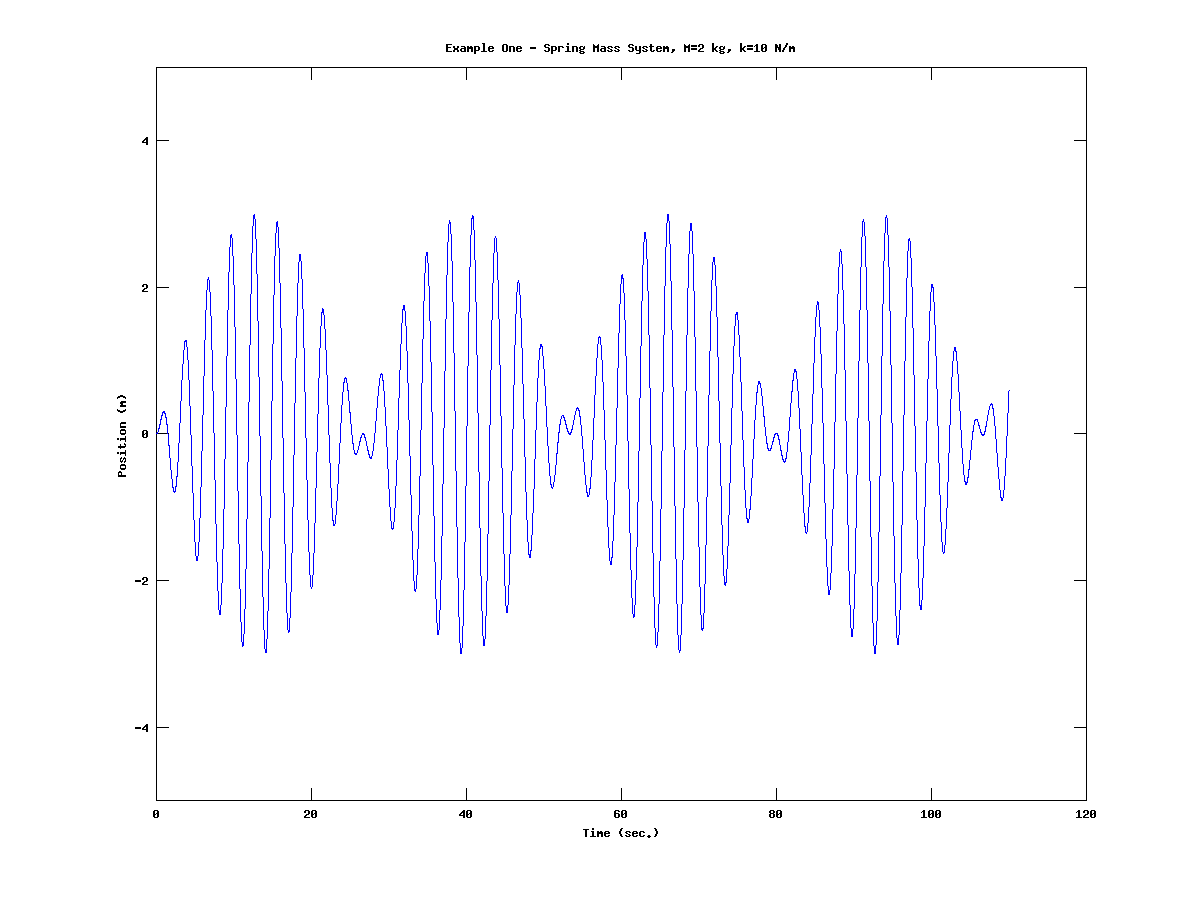
\includegraphics[width=11cm]{beats}}}
  \only<2>{\centerline{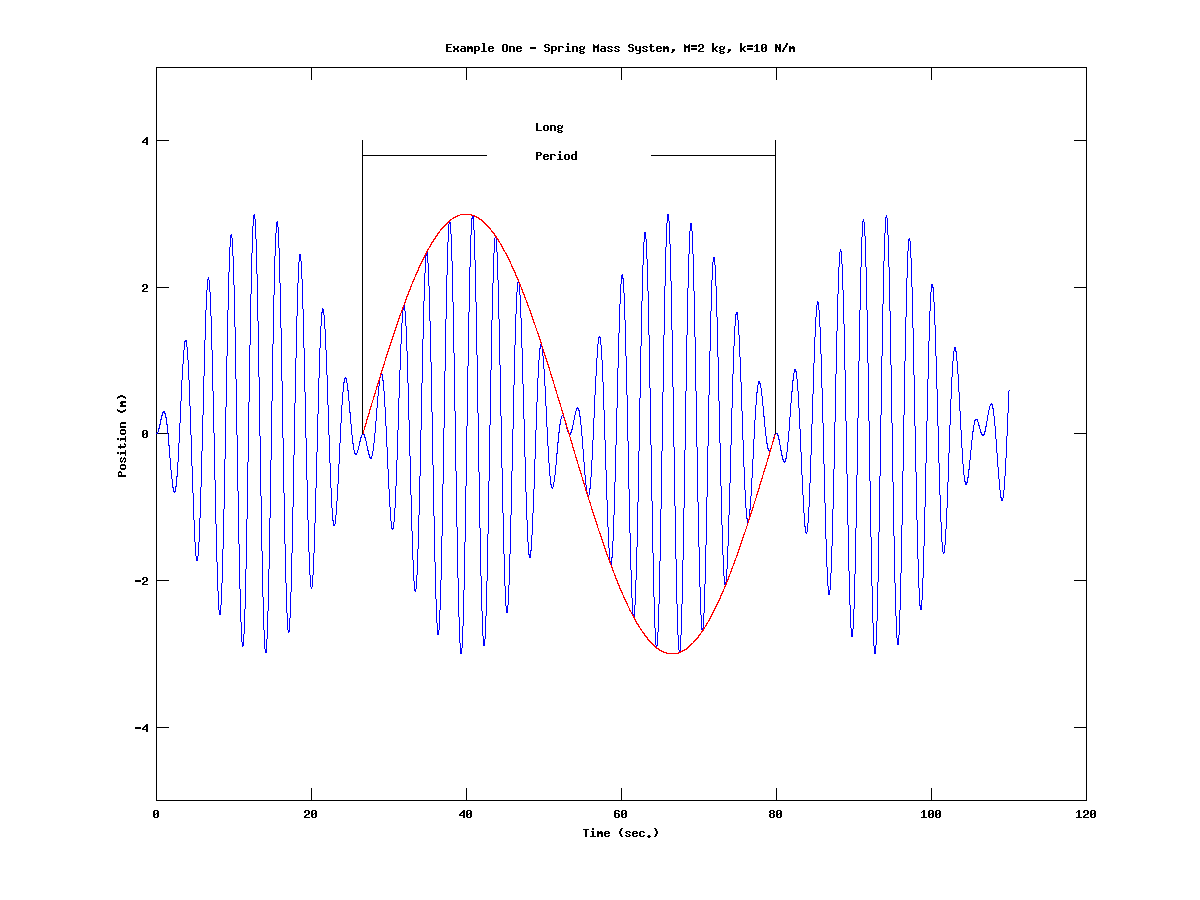
\includegraphics[width=11cm]{beatsLong}}}
  \only<3>{\centerline{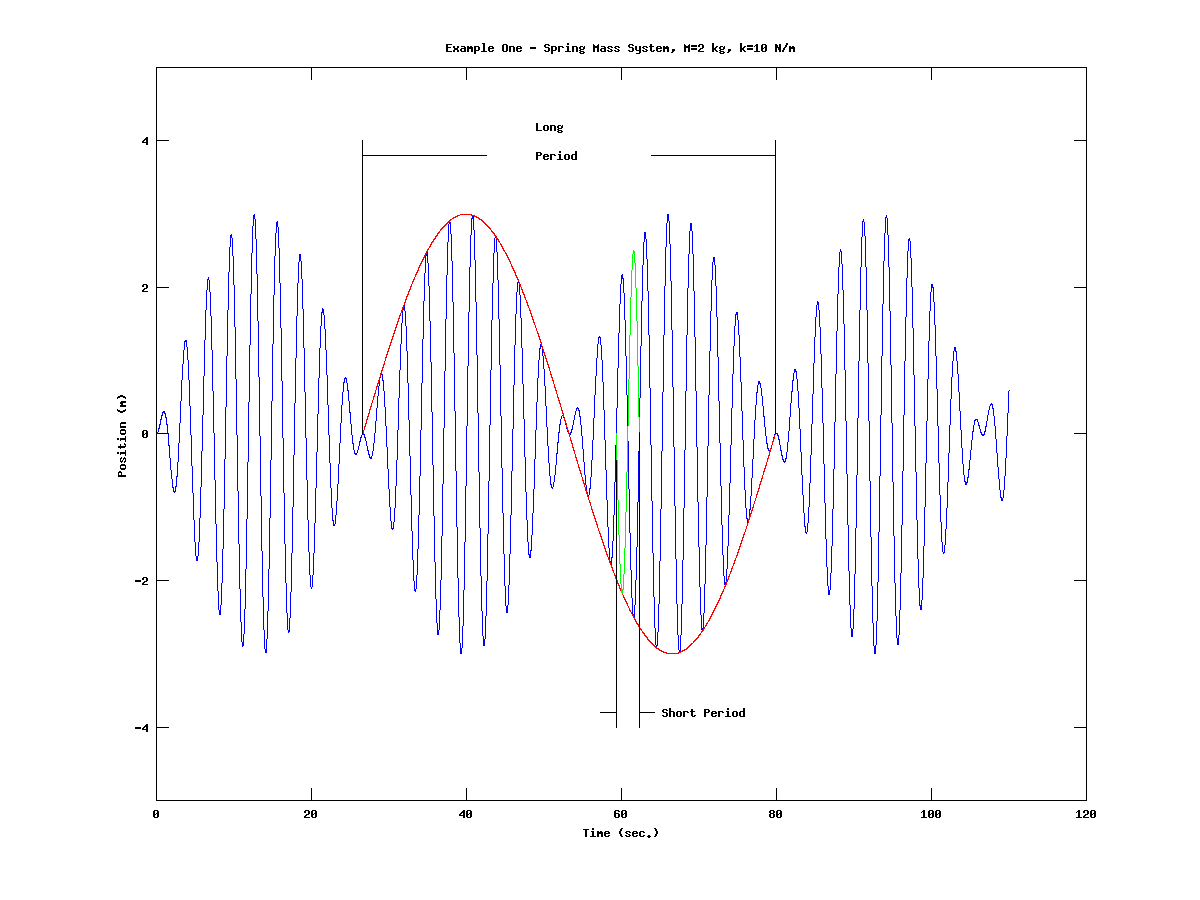
\includegraphics[width=11cm]{beatsShort}}}


\end{frame}




% LocalWords:  Clarkson pausesection hideallsubsections




% %%%%%%%%%%%%%%%%%%%%%%%%%%%%%%%%%%%%%%%%%%%%%%%%%%%%%%%%%%%%


\part{Eigen-Vectors/Values}
\lecture{Eigen Vectors/Values}{Eigen-Vectors/Values}


\title{Ordinary Differential Equations}
\subtitle{Math 232 - Week 10, Day 3}

\author{Kelly Black}
\institute{Clarkson University}
\date{4 November 2011}

\begin{frame}
  \titlepage
\end{frame}

\begin{frame}
  \frametitle{Outline}
  \tableofcontents[pausesection,hideallsubsections]
\end{frame}


\section{Eigen Vectors and Eigen Values}


\begin{frame}
  \frametitle{Eigen Vectors and Eigen Values}

  Suppose that we have a system of differential equations,
  \begin{eqnarray*}
    \frac{d}{dt} \vec{x} & = & A \vec{x}.
  \end{eqnarray*}
  Assume that $A$ is a square matrix.

  What if we can find a vector, $\vec{v}$, that satisfies
  \begin{eqnarray*}
    A \vec{v} & = & \lambda \vec{v},
  \end{eqnarray*}
  where $\lambda$ is a scalar number?

\end{frame}


\begin{frame}
  If so. then....
  \begin{eqnarray*}
    \frac{d}{dt} \vec{v} & = & A \vec{v}, \\
    & = & \lambda \vec{v}.
  \end{eqnarray*}
  
  This implies that
  \begin{eqnarray*}
    \deriv{x_1}{t} & = & \lambda x_1, \\
    \deriv{x_2}{t} & = & \lambda x_2, \\
    \deriv{x_3}{t} & = & \lambda x_3, \\
    \vdots         &   & \vdots \\
    \deriv{x_n}{t} & = & \lambda x_n
  \end{eqnarray*}

  We can solve each one of these equations separately!

\end{frame}


\begin{frame}
  \frametitle{Eigen Vectors and Eigen Values}

  Definition: Given a square matrix, $A$, an eigen vector, $\vec{v}$, and an
  eigen value, $\lambda$, satisfy
  \begin{eqnarray*}
    A \vec{v} & = & \lambda \vec{v}.
  \end{eqnarray*}

  Given $A$ how can we find them?

\end{frame}


\begin{frame}
  \frametitle{How to find}

  \begin{eqnarray*}
    A \vec{v} & = & \lambda \vec{v}, \\
    A \vec{v} - \lambda \vec{v} & = & 0, \\
    A \vec{v} - \lambda I \vec{v} & = & 0, \\
    \lp A - \lambda I \rp \vec{v} & = & 0.
  \end{eqnarray*}

  One solution is $\vec{v}=\vec{0}$. We do not like this solution. We
  must have a situation where there is not a unique solution. If there
  is not a unique solution then this implies that
  \begin{eqnarray*}
    \det\lp A - \lambda I \rp & = & 0.
  \end{eqnarray*}
  Find a value for $\lambda$ that makes this true. (Note that there
  will be infinite solutions for $\vec{v}$.)

\end{frame}


\begin{frame}
  \frametitle{Finding Eigen Vectors and Eigen Values}

  Given a square matrix, $A$, to find the eigen vectors and eigen
  values do the following:
  \begin{enumerate}
  \item Determine the characteristic equation:
    \begin{eqnarray*}
      \det\lp A - \lambda I \rp & = & 0.
    \end{eqnarray*}
  \item Solve the equation for the values of $\lambda$.
  \item Find the eigen vector associated with each value of $\lambda$,
    \begin{eqnarray*}
      \lp A - \lambda_j I \rp \vec{v}_j & = & \vec{0}.
    \end{eqnarray*}
    (Note that there will be infinite solutions for $\vec{v}$.)
  \end{enumerate}

\end{frame}

\section{Examples}

\begin{frame}
  \frametitle{Example}

  \begin{eqnarray*}
    A & = & \arrayTwo{12}{-10}{15}{-13}.
  \end{eqnarray*}

  Find the characteristic equation:
  \begin{eqnarray*}
    \det\lp\arrayTwo{12-\lambda}{-10}{15}{-13-\lambda}\rp & = & \lambda^2+\lambda-6.
  \end{eqnarray*}

  Find the values of $\lambda$:
  \begin{eqnarray*}
    \lambda^2+\lambda-6 & = & (\lambda-2)(\lambda+3), \\
    & = & 0.
  \end{eqnarray*}
  So $\lambda_1 = -3$ and $\lambda_2=2$.

\end{frame}


\begin{frame}
  Find the vectors:

  $\lambda_1 = 2$:
  \begin{eqnarray*}
    \arrayTwo{10}{-10}{15}{-15} \vecTwo{x}{y} & = & \vecTwo{0}{0}, \\
    10x - 10y & = & 0, \\
    15x - 15y & = & 0, \\
    x & = & y.
  \end{eqnarray*}

  The first eigen vector is 
  \begin{eqnarray*}
    \vec{v}_1 & = & \vecTwo{y}{y}, \\
    & = & y \vecTwo{1}{1}.
  \end{eqnarray*}

  Let
  \begin{eqnarray*}
    \vec{v}_1 & = & \vecTwo{1}{1}.
  \end{eqnarray*}

\end{frame}

\begin{frame}
  Find the vectors:

  $\lambda_2 = -3$:
  \begin{eqnarray*}
    \arrayTwo{15}{-10}{15}{-10} \vecTwo{x}{y} & = & \vecTwo{0}{0}, \\
    15x - 10y & = & 0, \\
    15x - 10y & = & 0, \\
    x & = & \frac{2}{3} y.
  \end{eqnarray*}

  The second eigen vector is 
  \begin{eqnarray*}
    \vec{v}_2 & = & \vecTwo{\frac{2}{3}y}{y}, \\
    & = & y \vecTwo{\frac{2}{3}}{1}.
  \end{eqnarray*}

  Let
  \begin{eqnarray*}
    \vec{v}_2 & = & \vecTwo{2}{3}.
  \end{eqnarray*}

\end{frame}






\begin{frame}
  \frametitle{Example}

  \begin{eqnarray*}
    A & = & \arrayTwo{4}{18}{-3}{-11}.
  \end{eqnarray*}

  Find the characteristic equation:
  \begin{eqnarray*}
    \det\lp\arrayTwo{4-\lambda}{18}{-3}{-11-\lambda}\rp & = & \lambda^2+7\lambda+10.
  \end{eqnarray*}

  Find the values of $\lambda$:
  \begin{eqnarray*}
    \lambda^2+7\lambda+10 & = & (\lambda+2)(\lambda+5), \\
    & = & 0.
  \end{eqnarray*}
  So $\lambda_1 = -2$ and $\lambda_2=-5$.


\end{frame}


\begin{frame}
  Find the vectors:

  $\lambda_1 = -2$:
  \begin{eqnarray*}
    \arrayTwo{6}{18}{-3}{-9} \vecTwo{x}{y} & = & \vecTwo{0}{0}, \\
    6x + 18y & = & 0, \\
    -3x - 9y & = & 0, \\
    x & = & -3y.
  \end{eqnarray*}

  The first eigen vector is 
  \begin{eqnarray*}
    \vec{v}_1 & = & \vecTwo{-3y}{y}, \\
    & = & y \vecTwo{-3}{1}.
  \end{eqnarray*}

  Let
  \begin{eqnarray*}
    \vec{v}_1 & = & \vecTwo{-3}{1}.
  \end{eqnarray*}

\end{frame}

\begin{frame}
  Find the vectors:

  $\lambda_2 = -5$:
  \begin{eqnarray*}
    \arrayTwo{9}{18}{-3}{-6} \vecTwo{x}{y} & = & \vecTwo{0}{0}, \\
    9x + 18y & = & 0, \\
    -3x - 6y & = & 0, \\
    x & = & -2 y.
  \end{eqnarray*}

  The second eigen vector is 
  \begin{eqnarray*}
    \vec{v}_2 & = & \vecTwo{-2y}{y}, \\
    & = & y \vecTwo{-2}{1}.
  \end{eqnarray*}

  Let
  \begin{eqnarray*}
    \vec{v}_2 & = & \vecTwo{-2}{1}.
  \end{eqnarray*}

\end{frame}



\begin{frame}
  \frametitle{Theorem - Distinct Eigen Values Makes Life Easier}

  Theorem: If the eigen values of an $n\times n$ matrix include $n$
  distinct values then the eigen vectors are linearly independent.

  \vfill

  \uncover<2->
  {
    So what? When we start solving DEs it will mean we are essentially
    done. 
  }

  \vfill

\end{frame}



\begin{frame}
  \frametitle{Example}

  See example 5 on page 318.
  \begin{eqnarray*}
    A & = & \arrayThree{-2}{1}{1}{1}{-2}{1}{1}{1}{-2}.
  \end{eqnarray*}

  Find the characteristic equation:
  \begin{eqnarray*}
    \det\lp\arrayThree{-2-\lambda}{1}{1}{1}{-2-\lambda}{1}{1}{1}{-2-\lambda}\rp
    & = & \lambda (\lambda+3)^2.
  \end{eqnarray*}

  Find the values of $\lambda$:
  \begin{eqnarray*}
    \lambda (\lambda+3)^2 & = & 0.
  \end{eqnarray*}
  So $\lambda_1 = 0$ and $\lambda_2=-3$.


\end{frame}


\begin{frame}
  Find the vectors:

  $\lambda_1 = 0$:
  \begin{eqnarray*}
    \arrayThree{-2}{1}{1}{1}{-2}{1}{1}{1}{-2}\vecThree{x}{y}{z} & = & \vecThree{0}{0}{0}, \\
  \end{eqnarray*}

  Express this system in an augmented matrix and put it in reduced row
  echelon form:
  \begin{eqnarray*}
    \mathrm{RREF}\startRowFour
    \oneRowFour{-2}{1}{1}{0} 
    \oneRowFour{1}{-2}{1}{0}
    \oneRowFour{1}{1}{-2}{0}
    \stopRowOps
    & = & 
    \startRowFour
    \oneRowFour{1}{0}{-1}{0} 
    \oneRowFour{0}{1}{-1}{0}
    \oneRowFour{0}{0}{0}{0}
    \stopRowOps
  \end{eqnarray*}


\end{frame}

\begin{frame}
  The first eigen vector is 
  \begin{eqnarray*}
    \vec{v}_1 & = & \vecThree{z}{z}{z}, \\
    & = & z \vecThree{1}{1}{1}.
  \end{eqnarray*}

  Let
  \begin{eqnarray*}
    \vec{v}_1 & = & \vecThree{1}{1}{1}.
  \end{eqnarray*}

\end{frame}

\begin{frame}
  Find the vectors:

  $\lambda_2 = -3$:
  \begin{eqnarray*}
    \arrayThree{1}{1}{1}{1}{1}{1}{1}{1}{1}
    \vecThree{x}{y}{z} & = & \vecThree{0}{0}{0}, \\
  \end{eqnarray*}

  Express this system in an augmented matrix and put it in reduced row
  echelon form:
  \begin{eqnarray*}
    \mathrm{RREF}\startRowFour
    \oneRowFour{1}{1}{1}{0} 
    \oneRowFour{1}{1}{1}{0}
    \oneRowFour{1}{1}{1}{0}
    \stopRowOps
    & = & 
    \startRowFour
    \oneRowFour{1}{1}{1}{0} 
    \oneRowFour{0}{0}{0}{0}
    \oneRowFour{0}{0}{0}{0}
    \stopRowOps
  \end{eqnarray*}

\end{frame}

\begin{frame}

  The second eigen vector is 
  \begin{eqnarray*}
    \vec{v}_2 & = & \vecThree{-y-z}{y}{z}, \\
    & = & y \vecThree{-1}{1}{0} + z \vecThree{-1}{0}{1}.
  \end{eqnarray*}

  Let
  \begin{eqnarray*}
    \vec{v}_2 & = & \vecThree{-1}{1}{0}, \\
    \vec{v}_3 & = & \vecThree{-1}{0}{1}.
  \end{eqnarray*}

\end{frame}



\begin{frame}
  \frametitle{Example}

  \begin{eqnarray*}
    A & = & \arrayThree{2}{1}{1}{0}{1}{1}{0}{0}{1}.
  \end{eqnarray*}

  Find the characteristic equation:
  \begin{eqnarray*}
    \det\lp\arrayThree{2-\lambda}{1}{1}{0}{1-\lambda}{1}{0}{0}{1-\lambda}\rp
    & = & (2-\lambda) (1-\lambda)^2.
  \end{eqnarray*}

  Find the values of $\lambda$:
  \begin{eqnarray*}
    (2-\lambda) (1-\lambda)^2 & = & 0.
  \end{eqnarray*}
  So $\lambda_1 = 2$ and $\lambda_2=1$.


\end{frame}


\begin{frame}
  Find the vectors:

  $\lambda_1 = 2$:
  \begin{eqnarray*}
    \arrayThree{0}{1}{1}{0}{-1}{1}{0}{0}{-1}\vecThree{x}{y}{z} & = & \vecThree{0}{0}{0}, \\
  \end{eqnarray*}

  Express this system in an augmented matrix and put it in reduced row
  echelon form:
  \begin{eqnarray*}
    \mathrm{RREF}\startRowFour
    \oneRowFour{0}{1}{1}{0} 
    \oneRowFour{0}{-1}{1}{0}
    \oneRowFour{0}{0}{-1}{0}
    \stopRowOps
    & = & 
    \startRowFour
    \oneRowFour{0}{1}{0}{0} 
    \oneRowFour{0}{0}{1}{0}
    \oneRowFour{0}{0}{0}{0}
    \stopRowOps
  \end{eqnarray*}


\end{frame}

\begin{frame}
  The first eigen vector is 
  \begin{eqnarray*}
    \vec{v}_1 & = & \vecThree{x}{0}{0}, \\
    & = & x \vecThree{1}{0}{0}.
  \end{eqnarray*}

  Let
  \begin{eqnarray*}
    \vec{v}_1 & = & \vecThree{1}{0}{0}.
  \end{eqnarray*}

\end{frame}

\begin{frame}
  Find the vectors:

  $\lambda_2 = 1$:
  \begin{eqnarray*}
    \arrayThree{1}{1}{1}{0}{0}{1}{0}{0}{0}
    \vecThree{x}{y}{z} & = & \vecThree{0}{0}{0}, \\
  \end{eqnarray*}

  Express this system in an augmented matrix and put it in reduced row
  echelon form:
  \begin{eqnarray*}
    \mathrm{RREF}\startRowFour
    \oneRowFour{1}{1}{1}{0} 
    \oneRowFour{0}{0}{1}{0}
    \oneRowFour{0}{0}{0}{0}
    \stopRowOps
    & = & 
    \startRowFour
    \oneRowFour{1}{1}{0}{0} 
    \oneRowFour{0}{0}{1}{0}
    \oneRowFour{0}{0}{0}{0}
    \stopRowOps
  \end{eqnarray*}

\end{frame}

\begin{frame}

  The second eigen vector is 
  \begin{eqnarray*}
    \vec{v}_2 & = & \vecThree{-y}{y}{0}, \\
    & = & y \vecThree{-1}{1}{0}.
  \end{eqnarray*}

  Let
  \begin{eqnarray*}
    \vec{v}_2 & = & \vecThree{-1}{1}{0}.
  \end{eqnarray*}

  There are only two eigen vectors!

\end{frame}




% LocalWords:  Clarkson pausesection hideallsubsections Eigen eigen



% %%%%%%%%%%%%%%%%%%%%%%%%%%%%%%%%%%%%%%%%%%%%%%%%%%%%%%%%%%%%


\part{Systems-of-DEs}
\lecture{Systems of DEs}{Systems-of-DEs}
\section{Systems of DEs}


\title{Ordinary Differential Equations}
\subtitle{Math 232 - Week 11, Day 1}
\date{7 November 2012}

\begin{frame}
  \titlepage
\end{frame}

\begin{frame}
  \frametitle{Outline}
  \tableofcontents[pausesection,hideothersubsections]
\end{frame}


\subsection{Systems of Differential Equations}


\begin{frame}
  \frametitle{Systems of Differential Equations}

  Conceptual Model: Automobile Suspension

  \begin{eqnarray*}
    \deriv{~}{t} \lp m \vec{v_1} \rp & = & \sum_j \vec{F}_{1j} \\
    \deriv{~}{t} \lp m \vec{v_2} \rp & = & \sum_j \vec{F}_{2j} 
  \end{eqnarray*}

\end{frame}


\begin{frame}
  \frametitle{Start at the Beginning}

  \begin{eqnarray*}
    \deriv{~}{t} x_1  & = & a_{11} x_1 + a_{12} x_2 + f_1(t), \\
    \deriv{~}{t} x_2  & = & a_{21} x_1 + a_{22} x_2 + f_2(t).
  \end{eqnarray*}

  Writing the system in matrix/vector form we get
  \begin{eqnarray*}
    \deriv{~}{t} \vecTwo{x_1}{x_2} & = & 
    \arrayTwo{a_{11}}{a_{12}}{a_{21}}{a_{22}} \vecTwo{x_1}{x_2} + 
    \vecTwo{f_1}{f_2}.
  \end{eqnarray*}

\end{frame}


\begin{frame}
  \frametitle{More General Notation}

  \begin{eqnarray*}
    \deriv{~}{t} \vec{x}(t) & = & A(t) \vec{x}(t) + \vec{f}(t), \\
    \deriv{~}{t} \vec{x} & = & A \vec{x} + \vec{f}, \\
    \vec{x}(t_0) & = & 
    \left[
      \begin{array}{r}
        c_1 \\ c_2 \\ \vdots \\ c_n
      \end{array}
    \right]
  \end{eqnarray*}

  Definition: if $\vec{f}=\vec{0}$ then the system of equations is
  homogeneous.

  \begin{itemize}
  \item Solutions are the sum of homogeneous and particular solutions.
  \item Solutions are found by assuming a general form and then
    searching for the ``right answer.''
  \end{itemize}

\end{frame}

\subsection{Example}

\begin{frame}
  \frametitle{Example}

  \begin{eqnarray*}
    \deriv{~}{t} x_1 & = & 5  x_1 + 24 x_2 + 8 e^{-11t}, \\
    \deriv{~}{t} x_2 & = & -2 x_1 -  9 x_2 + 4 e^{-11t}.
  \end{eqnarray*}

  \uncover<2->
  {
    Written in matrix/vector form we get
    \begin{eqnarray*}
      \deriv{~}{t} \vecTwo{x_1}{x_2} & = & 
      \arrayTwo{5}{24}{-2}{-9} \vecTwo{x_1}{x_1}
      + \vecTwo{8e^{-11t}}{4e^{-11t}}.
    \end{eqnarray*}
  }

  \uncover<3->
  {
    The solution is
    \begin{eqnarray*}
      \vec{x} & = & C_1 e^{-t} \vecTwo{4}{-1} 
      + C_2 e^{-3t} \vecTwo{-3}{1} + e^{-11t} \vecTwo{1}{-1}.
    \end{eqnarray*}
  }

\end{frame}


\begin{frame}[allowframebreaks]
  \frametitle{Notes}

  \begin{enumerate}
  \item
    \begin{eqnarray*}
      \vec{x}_h & = & C_1 e^{-t} \vecTwo{4}{-1} 
      + C_2 e^{-3t} \vecTwo{-3}{1}.
    \end{eqnarray*}


    i.e.
    \begin{eqnarray*}
      \deriv{~}{t} \vec{x}_h & = & \arrayTwo{5}{24}{-2}{-9} \vec{x}_h.
    \end{eqnarray*}

  \item
    \begin{eqnarray*}
      \vec{x}_p & = & e^{-11t} \vecTwo{1}{-1}.
    \end{eqnarray*}

  \item The homogeneous solution is made up of two vectors, and this
    is a $2\times 2$ system.

  \item 
    \begin{eqnarray*}
      \vec{x}_h & = &
      \underbrace{\arrayTwo{4e^{-t}}{-3e^{-3t}}{-e^{-t}}{e^{-3t}}}_{\mathrm{Fundamental~Matrix}}
      \vecTwo{C_1}{C_2} 
    \end{eqnarray*}

  \item The vectors $\vecTwo{4}{-1}$ and $\vecTwo{-3}{1}$ are linearly
    independent.

  \item
    \begin{eqnarray*}
      \arrayTwo{5}{24}{-2}{-9} \vecTwo{4}{-1} & = & - \vecTwo{4}{-1}, \\
      \arrayTwo{5}{24}{-2}{-9} \vecTwo{-3}{1} & = & -3 \vecTwo{-3}{1}.
    \end{eqnarray*}



  \end{enumerate}

\end{frame}

\subsection{General Framework}

\begin{frame}
  \frametitle{General Solutions}

  \begin{eqnarray*}
    \deriv{~}{t} \vec{x}  & = & A \vec{x} + \vec{f}(t), \\
    \vec{x} & = & \vec{x}_h + \vec{x}_p, \\
    \vec{x}_h & = & \underbrace{C_1 \vec{x}_1(t) + C_2 \vec{x}_2(t) + \cdots + C_n \vec{x}_n(t)}_{n~\mathrm{linearly~independent~vectors}}, \\
    \vec{x}_h & = & \left[ \vec{x_1} \bigg| \vec{x_2} \bigg| \cdots \bigg| \vec{x_n} \right]
    \left[
      \begin{array}{rr}
        C_1 \\ C_2 \\ \vdots \\ C_n
      \end{array}
    \right].
  \end{eqnarray*}

  The vectors, $\vec{x}_i$, are related to the eigen values and the eigen vectors.

\end{frame}


\begin{frame}
  \frametitle{The Phase Plane}

  In our example, the solution looks like
  \begin{eqnarray*}
    \vec{x}(t) & = & \vecTwo{x(t)}{y(t)}.
  \end{eqnarray*}
  This is a path in the plane.

  \begin{itemize}
  \item One solution represented as a path in the plane is a \textit{solution graph}.
  \item Many solutions represented as paths in the plane is the \textit{phase plane}.
  \item If the solutions are unique then they cannot cross.
  \end{itemize}

\end{frame}

\subsection{Reducing High Order Systems Using Systems}

\begin{frame}
  \frametitle{Tricks of the Trade}

  Suppose that we have
  \begin{eqnarray*}
    x'' + 3x' + 2x & = & 0. \\
    \uncover<2->
    {
      \Rightarrow r^2 + 3r + 2 & = & 0, \\
      (r+2)(r+1) & = & 0, \\
      x & = & a e^{-2t} + b e^{-t}.
    }
  \end{eqnarray*}

\end{frame}


\begin{frame}
  \frametitle{Another Way to Look at It}

  We have
  \begin{eqnarray*}
    x'' + 3x' + 2x & = & 0.
  \end{eqnarray*}

  Let
  \begin{eqnarray*}
    y & = & x', \\
    \uncover<2->
    {
      x'' & = & y', \\
      y' & = & -2x - 3x', \\
      & = & -2x - 3y.
    }
  \end{eqnarray*}

  \uncover<3->
  {
    Written in matrix/vector form we get
    \begin{eqnarray*}
      \deriv{~}{t} \vecTwo{x}{y} & = & \arrayTwo{0}{1}{-2}{-3} \vecTwo{x}{y}.
    \end{eqnarray*}
  }


\end{frame}

\begin{frame}
  \frametitle{Find the Eigen Values and Eigen Vectors}

  \begin{eqnarray*}
    A & = & \arrayTwo{0}{1}{-2}{-3}.
  \end{eqnarray*}

  \uncover<2->
  {
    \begin{eqnarray*}
      \begin{array}{rcl@{\hspace{2em}}rcl}
          \lambda_1 & = & -1, & \vec{v}_1 & = & \vecTwo{1}{-1}, \\
          \lambda_2 & = & -2, & \vec{v}_2 & = & \vecTwo{-1}{2}.
        \end{array}
    \end{eqnarray*}
  }

  \uncover<3->
  {
    The solution is
    \begin{eqnarray*}
      \vec{x}(t) & = & C_1 e^{-t} \vecTwo{1}{-1}  + C_2 e^{-2t} \vecTwo{-1}{2}, \\
      x & = & C_1 e^{-t} - C_2 e^{-2t}, \\
      y & = & -C_1 e^{-t} + 2 C_2 e^{-2t}.
    \end{eqnarray*}
  }

\end{frame}


% LocalWords:  Clarkson pausesection hideothersubsections


\part{Solutions-to-Systems-of-DEs}
\lecture{Solutions to Systems of DEs}{Solutions-to-Systems-of-DEs}
\section{Solutions to Systems of DEs}


\title{Ordinary Differential Equations}
\subtitle{Math 232 - Week 11, Day 2}
\date{9 November 2011}

\begin{frame}
  \titlepage
\end{frame}

\begin{frame}
  \frametitle{Outline}
  \tableofcontents[pausesection,hideothersubsections]
\end{frame}


\subsection{Solutions to Systems of DEs}


\begin{frame}
  \frametitle{What is a solution to a System of DEs?}

  \begin{eqnarray*}
    \deriv{~}{t} \vec{x} & = & A \vec{x}.
  \end{eqnarray*}

  \uncover<2->
  {
    Assume that 
    \begin{eqnarray*}
      \vec{x} & = & c e^{\lambda t} \vec{v}.
    \end{eqnarray*}
  }


\end{frame}


\begin{frame}
  \frametitle{Substitute it into the equation}

  \begin{eqnarray*}
    \deriv{~}{t} \vec{x} & = & c \lambda e^{\lambda t} \vec{v} \\
    \Rightarrow c  e^{\lambda t} A \vec{v} & = & c \lambda e^{\lambda t} \vec{v}, \\
    A \vec{v} & = & \lambda \vec{v}.
  \end{eqnarray*}

  This is an eigen vector/eigen value problem!

\end{frame}


\begin{frame}
  \frametitle{Homogeneous Equations}

  Given
  \begin{eqnarray*}
    \deriv{~}{t} \vec{x} & = & A \vec{x},
  \end{eqnarray*}
  where $A$ is an $n\times n$ matrix, find the eigen vectors and eigen
  values. \textbf{If} there are $n$ linearly independent eigen vectors
  then 
  \begin{eqnarray*}
    \vec{x} & = & c_1 e^{\lambda_1 t} \vec{v}_1 + c_2 e^{\lambda_2 t} \vec{v}_2 +
    \cdot + c_n e^{\lambda_n t} \vec{v}_n.
  \end{eqnarray*}

\end{frame}

\subsection{Examples}

\begin{frame}
  \frametitle{Example}

  \begin{eqnarray*}
    \deriv{~}{t} \vec{x} & = & \arrayTwo{5}{24}{-2}{-9} \vec{x}.
  \end{eqnarray*}

  \uncover<2->
  {
    First find the eigen values,
    \begin{eqnarray*}
      0 & = & \det\lp\arrayTwo{5-\lambda}{24}{-2}{-9-\lambda}\rp, \\
      & = & (\lambda+2)(\lambda+1).
    \end{eqnarray*}
    The eigen values are $\lambda_1=-1$ and $\lambda_2=-3$.
  }

\end{frame}


\begin{frame}
  \frametitle{Find the eigen vectors}

  $\lambda_1 = -1$:
  \begin{eqnarray*}
    \arrayTwo{6}{24}{-2}{-8} \vecTwo{x}{y} & = & \vecTwo{0}{0}, \\
    6x + 24y & = & 0, \\
    -2x - 8y & = & 0, \\
    \uncover<2->
    {
      \Rightarrow \vec{v}_1 & = & \vecTwo{-4}{1}.
    }
  \end{eqnarray*}

  \uncover<3->
  {
    $\lambda_2 = -3$:
    \begin{eqnarray*}
      \arrayTwo{8}{24}{-2}{-6} \vecTwo{x}{y} & = & \vecTwo{0}{0}, \\
      8x + 24y & = & 0, \\
      -2x - 6y & = & 0, \\
      \uncover<4->
      {
        \Rightarrow \vec{v}_2 & = & \vecTwo{-3}{1}.
      }
    \end{eqnarray*}
  }

\end{frame}


\begin{frame}
  \frametitle{Assemble the Solution}

  \begin{eqnarray*}
    \vec{x}(t) & = & c_1 e^{-t} \vecTwo{-4}{1} + c_2 e^{-3t} \vecTwo{-3}{1}.
  \end{eqnarray*}

\end{frame}

\begin{frame}
  \frametitle{Example}

  \begin{eqnarray*}
    x'' + 5x' + 6x & = & 0, \\
    \Rightarrow x_h & = & C_1 e^{-3t} + C_2 e^{-2t}.
  \end{eqnarray*}

  Let $x'=y$,
  \begin{eqnarray*}
    x' & = & y, \\
    y' & = & -6x - 5y,
  \end{eqnarray*}
  which leads to the following system
  \begin{eqnarray*}
    \deriv{~}{t} \vec{x} & = & \arrayTwo{0}{1}{-6}{-5} \vec{x}.
  \end{eqnarray*}
\end{frame}

\begin{frame}
    \frametitle{First find the eigen values}
    \begin{eqnarray*}
      0 & = & \det\lp\arrayTwo{-\lambda}{1}{-6}{-5-\lambda}\rp, \\
      & = & (\lambda+2)(\lambda+3).
    \end{eqnarray*}
    The eigen values are $\lambda_1=-2$ and $\lambda_2=-3$.

\end{frame}


\begin{frame}
  \frametitle{Find the eigen vectors}

  $\lambda_1 = -2$:
  \begin{eqnarray*}
    \arrayTwo{2}{1}{-6}{-3} \vecTwo{x}{y} & = & \vecTwo{0}{0}, \\
    2x + y & = & 0, \\
    -6x - 3y & = & 0, \\
    \uncover<2->
    {
      \Rightarrow \vec{v}_1 & = & \vecTwo{1}{-2}.
    }
  \end{eqnarray*}

  \uncover<3->
  {
    $\lambda_2 = -3$:
    \begin{eqnarray*}
      \arrayTwo{3}{1}{-6}{-2} \vecTwo{x}{y} & = & \vecTwo{0}{0}, \\
      3x + y & = & 0, \\
      -6x - 2y & = & 0, \\
      \uncover<4->
      {
        \Rightarrow \vec{v}_2 & = & \vecTwo{1}{-3}.
      }
    \end{eqnarray*}
  }

\end{frame}


\begin{frame}
  \frametitle{Assemble the Solution}

  \begin{eqnarray*}
    \vec{x}(t) & = & c_1 e^{-2t} \vecTwo{1}{-2} + c_2 e^{-3t} \vecTwo{1}{-3}.
  \end{eqnarray*}

\end{frame}


\subsection{The Phase Plane}

\begin{frame}
  \frametitle{Phase Plane Solutions}


\end{frame}

\subsection{Repeated Eigen Values}

\begin{frame}
  \frametitle{Example}

  \begin{eqnarray*}
    \deriv{~}{t} \vec{x} & = & \arrayTwo{0}{-1}{4}{-4} \vec{x}.
  \end{eqnarray*}

  \uncover<2->
  {
    Find the eigen values:
    \begin{eqnarray*}
      0 & = & \det\lp\arrayTwo{-\lambda}{-1}{4}{-4-\lambda}\rp, \\
      & = & \lp \lambda + 2 \rp^2,
    \end{eqnarray*}
    The value of $\lambda$ is -2.
  }

\end{frame}


\begin{frame}
  \frametitle{Find the eigen vectors}

  \begin{eqnarray*}
    \arrayTwo{2}{1}{4}{2} \vec{x}{y} & = & \vecTwo{0}{0}, \\
    2x + y & = & 0, \\
    4x + 2y & = & 0.
  \end{eqnarray*}

  There is only one eigen vector,
  \begin{eqnarray*}
    \vec{v}_1 & = & \vecTwo{1}{-2}.
  \end{eqnarray*}

\end{frame}

\begin{frame}
  \frametitle{What to do?}

  Last time this happened we tried to multiply by $t$, and it
  worked. We will try that again...
  Assume that
  \begin{eqnarray*}
    \vec{x} & = & t e^{\lambda t} \vec{v} + e^{\lambda t} \vec{u}.
  \end{eqnarray*}

  \uncover<2->
  {
    Substitute back into the equation:
    \begin{eqnarray*}
      \deriv{~}{t} \vec{x} & = & \lambda t e^{\lambda t} \vec{v} + e^{\lambda t} \vec{v} 
         + \lambda e^{\lambda t} \vec{u}, \\
         & = & 
      \lambda t e^{\lambda t} \vec{v} + e^{\lambda t} \vec{v} + \lambda e^{\lambda t} \vec{u}, \\
      A\vec{x} & = & t e^{\lambda t} A \vec{v} + e^{\lambda t} A \vec{u}.
    \end{eqnarray*}
  }
  
\end{frame}


\begin{frame}
  \frametitle{Set The Two Expressions Equal}

    \begin{eqnarray*}
      \lambda t e^{\lambda t} \vec{v} + e^{\lambda t} \vec{v} + \lambda e^{\lambda t} \vec{u}
      & = & 
      t e^{\lambda t} A \vec{v} + e^{\lambda t} A \vec{u}.
    \end{eqnarray*}
  
    This has to be true for all $t$ so we have the following equations:
    \begin{eqnarray*}
      \lambda t e^{\lambda t} \vec{v} & = & t e^{\lambda t} A \vec{v}, \\
      \lambda \vec{v} & = & A \vec{v}.
    \end{eqnarray*}
    (This is the eigen value and eigen vector!)

    We also have 
    \begin{eqnarray*}
      e^{\lambda t} \vec{v} + \lambda e^{\lambda t} \vec{u} & = & e^{\lambda t} A \vec{u}, \\
      \vec{v} + \lambda \vec{u} & = &  A \vec{u}, \\
      \Rightarrow \lp A - \lambda I \rp \vec{u} & = & \vec{v}.
    \end{eqnarray*}

\end{frame}

\begin{frame}
  \frametitle{Back to the Example}

  In out example we have
  \begin{eqnarray*}
    \vec{x} & = & t e^{\lambda t} c_1 \vecTwo{1}{2} + e^{\lambda t} \vec{u}, \\
    \arrayTwo{2}{-1}{4}{-2} \vecTwo{x}{y} & = & \vecTwo{c_1}{2c_1}, \\
    2x-y & = & c_1 \\
    4x-2y & = & 2 c_1.
  \end{eqnarray*}

  The vector, $\vec{u}$, is the following:
  \begin{eqnarray*}
    \vec{u} & = & \vecTwo{c_2}{2c_2-c_1}.
  \end{eqnarray*}
  
\end{frame}

\begin{frame}
  \frametitle{Form the Solution}
  
  The solution to the differential equation is
  \begin{eqnarray*}
    \vec{x}(t) & = & t e^{-2t} c_1 \vecTwo{1}{2} + e^{-2t} \vecTwo{c_2}{2c_2-c_1}, \\
    & = & e^{-2t} c_1 \vecTwo{t}{2t-1} + e^{-2t} c_2 \vecTwo{1}{2}.
  \end{eqnarray*}
\end{frame}

\begin{frame}
  \frametitle{Example}

  \begin{eqnarray*}
    \deriv{~}{t} \arrayTwo{2}{0}{0}{2} \vec{x}.
  \end{eqnarray*}

  \uncover<2->
  {
    Find the eigen values,
    \begin{eqnarray*}
      0 & = & \det\lp\arrayTwo{2-\lambda}{0}{0}{2-\lambda}\rp, \\
      & = & (2-\lambda)^2.
    \end{eqnarray*}
    The eigen value is $\lambda=2$.
  }

\end{frame}

\begin{frame}
  \frametitle{Find the Eigen Vector}

  $\lambda_1=2$:
  \begin{eqnarray*}
    \arrayTwo{0}{0}{0}{0} \vecTwo{x}{y} & = & \vecTwo{0}{0}, \\
    \uncover<2->
    {
      \Rightarrow \vec{v} & = & \vecTwo{x}{y}, \\
      & = & x \vecTwo{1}{0} + y \vecTwo{0}{1}, \\
      \uncover<3->
      {
        \vec{v}_1 & = & \vecTwo{1}{0}, \\
        \vec{v}_2 & = & \vecTwo{0}{1}.
      }
    }
  \end{eqnarray*}
\end{frame}


\begin{frame}
  \frametitle{Form the Solution}
    
  The solution is 
  \begin{eqnarray*}
    \vec{x} & = & c_1 e^{2t} \vecTwo{1}{0} + c_2 e^{2t} \vecTwo{0}{1}.
  \end{eqnarray*}

\end{frame}


\subsection{Coupled Tank Problems}


\begin{frame}
  \frametitle{Coupled Tank}

  Two tanks are arranged as shown. Initially tank 1 has 100 liters of
  water and tank 2 has 50 liters of water. Initially each tank has 2
  kg of salt dissolved in the solution. Determine the amount of salt
  in each tank at any time.
  
\end{frame}


\begin{frame}
  \frametitle{System of Equations}

  $x(t)$ is the amount of salt in tank 1 at time $t$.

  $y(t)$ is the amount of salt in tank 2 at time $t$.

  \begin{eqnarray*}
    \deriv{x}{t} & = & 0\times 2 - 
    \frac{x}{100}\times 3 + \frac{y}{50}\times 2 \\
    \deriv{y}{t} & = & \frac{x}{100} \times 3 -
    \frac{y}{50} \times 1 - \frac{y}{50}\times 2.
  \end{eqnarray*}

  Written as a system we get
  \begin{eqnarray*}
    \deriv{~}{t} \vecTwo{x}{y} & = & 
    \arrayTwo{-3/100}{1/50}{3/100}{-3/50} \vecTwo{x}{y}.
  \end{eqnarray*}
  
\end{frame}


% LocalWords:  Clarkson pausesection hideothersubsections


\part{Complex-Eigen-Values}
\lecture{Complex Eigen Values}{Complex-Eigen-Values}
\section{Complex Eigen Values}


\title{Ordinary Differential Equations}
\subtitle{Math 232 - Week 11, Day 3}
\date{11 November 2012}

\begin{frame}
  \titlepage
\end{frame}

\begin{frame}
  \frametitle{Outline}
  \tableofcontents[pausesection,hideothersubsections]
\end{frame}


\subsection{Complex Valued Eigen Values}


\begin{frame}
  \frametitle{Complex Valued Eigen Values}

  First, recall:
  \begin{eqnarray*}
    e^{a+bi} & = & e^a e^{bi}, \\
    & = & e^a \lp \cos(b) + i \sin(b) \rp.
  \end{eqnarray*}

  Also, the complex conjugate:
  \begin{eqnarray*}
    \overline{a+ib} & = & a-i b.
  \end{eqnarray*}

  Note: If A is a real valued matrix with complex valued eigen values,
  then the eigen values and eigen vectors come in complex conjugates
  pairs.

\end{frame}


\begin{frame}
  \frametitle{Example}

  \begin{eqnarray*}
    \deriv{~}{t} \vec{x} & = & \arrayTwo{5}{-10}{1}{-1} \vec{x}.
  \end{eqnarray*}

  \uncover<2->
  {
    Find the eigen values:
    \begin{eqnarray*}
      \det\lp\arrayTwo{5-\lambda}{-10}{1}{-1-\lambda}\rp & = & \lambda^2-4 \\
      \lambda_{1,2} & = & 2 \pm i.
    \end{eqnarray*}
  }

\end{frame}


\begin{frame}
  \frametitle{Find the Eigen Vectors}

  $\lambda_1 = 2+i$:
  \begin{eqnarray*}
    \arrayTwo{3-i}{-10}{1}{-3-i} \vecTwo{x}{y} & = & \vecTwo{0}{0} \\
    y & = & \lp \frac{3}{10} - \frac{i}{10} \rp x, \\
    \Rightarrow \vec{v}_1 & = & x \lp \vecTwo{1}{\frac{3}{10}} + \vecTwo{0}{\frac{-i}{10}} \rp.
  \end{eqnarray*}

  \uncover<2->
  {
    $\lambda_2 = 2-i$:
    \begin{eqnarray*}
      \arrayTwo{3+i}{-10}{1}{-3+i} \vecTwo{x}{y} & = & \vecTwo{0}{0} \\
      y & = & \lp \frac{3}{10} + \frac{i}{10} \rp x, \\
      \Rightarrow \vec{v}_2 & = & x \lp \vecTwo{1}{\frac{3}{10}} + \vecTwo{0}{\frac{i}{10}} \rp.
    \end{eqnarray*}
  }

\end{frame}


\begin{frame}
  \frametitle{Determine the Solution}

  \begin{eqnarray*}
    \uncover<1->
    {
      \vec{x} & = & A e^{(2+i)t} \lp \vecTwo{1}{\frac{3}{10}} + \vecTwo{0}{\frac{-i}{10}} \rp
      + B e^{(2-i)t} \lp \vecTwo{1}{\frac{3}{10}} - \vecTwo{0}{\frac{-i}{10}} \rp \\
    }
    \uncover<2->
    {
      \vec{x} & = & A e^{(2+i)t} \lp \underbrace{\vecTwo{1}{\frac{3}{10}}}_{\vec{p}} + 
      \underbrace{\vecTwo{0}{\frac{-i}{10}}}_{i\vec{q}} \rp
      + B e^{(2-i)t} \lp \underbrace{\vecTwo{1}{\frac{3}{10}}}_{\vec{p}} -
      \underbrace{\vecTwo{0}{\frac{-i}{10}}}_{i\vec{q}} \rp \\
    }
    \uncover<3->
    {
      & = & e^{2t} \lp
      A\lp \cos(t) + i \sin(t) \rp \lp \vec{p} + i \vec{q} \rp 
      + B \lp \cos(t) - i \sin(t) \rp \lp \vec{p} - i \vec{q} \rp 
      \rp
    }
  \end{eqnarray*}

\end{frame}


\begin{frame}
  \frametitle{More Algebra...}

  \begin{eqnarray*}
    \vec{x} & = & e^{2t} \lp
      A\lp \cos(t) + i \sin(t) \rp \lp \vec{p} + i \vec{q} \rp 
      + B \lp \cos(t) - i \sin(t) \rp \lp \vec{p} - i \vec{q} \rp 
      \rp \\
      & = & C_1 e^{2t} \lp \cos(t) \vec{p} - \sin(t) \vec{q} \rp
      + C_2 e^{2t} \lp \cos(t) \vec{q} + \sin(t) \vec{p} \rp.
  \end{eqnarray*}

  (The solutions spiral out.)

\end{frame}

\subsection{Characterization of Solutions}

\begin{frame}
  \frametitle{Characterization of Solutions}

  \begin{eqnarray*}
    \deriv{~}{t} \vec{x} & = & A \vec{x}.
  \end{eqnarray*}

  If $\lambda$'s are complex, $\lambda = a \pm ib$:
  \begin{enumerate}
  \item If $\alpha>0$ then it is a repelling spiral.
  \item If $\alpha<0$ then it is an attracting spiral.
  \item If $\alpha=0$ then the solutions are neutrally stable.
  \end{enumerate}

\end{frame}


\subsection{Nullclines}

\begin{frame}
  \frametitle{Nullclines}

  Given a solution to a differential equation,
  \begin{eqnarray*}
    \vec{x} & = & \vecTwo{x(t)}{y(t)},
  \end{eqnarray*}
  if
  \begin{itemize}
  \item $x'(t)=0$ then the trajectory is ``vertical'' at time $t$,
  \item $y'(t)=0$ then the trajectory is ``horizontal'' at time $t$.
  \end{itemize}

\end{frame}


\begin{frame}
  \frametitle{Definition of the Nullclines}

  The set of points, $\vecTwo{x}{y}$ where $x'(t)=0$ is called the v-nullcline. (Vertical slope.)

  The set of points, $\vecTwo{x}{y}$ where $y'(t)=0$ is called the h-nullcline. (Horizontal slope.)

\end{frame}


\begin{frame}
  \frametitle{Example}
  
  In the previous example we had
  \begin{eqnarray*}
    \deriv{~}{t} \vec{x} & = & \arrayTwo{5}{-10}{1}{-1} \vec{x}.
  \end{eqnarray*}

  \uncover<2->
  {
    Find the v-nullcline:
    \begin{eqnarray*}
      \deriv{x}{t} & = & 5x - 10y, \\
      0 & = & 5x - 10y, \\
      y & = & \frac{1}{2} x.
    \end{eqnarray*}
  }

  \uncover<3->
  {
    Find the h-nullcline:
    \begin{eqnarray*}
      \deriv{y}{t} & = & x - y, \\
      0 & = & x - y, \\
      y & = &  x.
    \end{eqnarray*}
  }


\end{frame}



% LocalWords:  Clarkson pausesection hideothersubsections



\title{Ordinary Differential Equations}
\subtitle{Math 232 - Week 12, Day 1}

\author{Kelly Black}
\institute{Clarkson University}
\date{14 November 2011}

\begin{frame}
  \titlepage
\end{frame}

\begin{frame}
  \frametitle{Outline}
  \tableofcontents[pausesection,hideallsubsections]
\end{frame}


\section{Behavior of Solutions to DEs}


\begin{frame}
  \frametitle{Behavior of Solutions to DEs}

  The eigen values determien the stability characteristics of the
  system of DEs.

  If the eigen values are real:
  \begin{itemize}
  \item $\lambda_2 < \lambda_1 < 0$ - Attracting
  \item $\lambda_2 < 0 < \lambda_1$ - Saddle
  \item $0 < \lambda_2 < \lambda_1$ - Repelling
  \end{itemize}

  If the eigen values are complex, $\lambda_{1,2}=a+ib$:
  \begin{itemize}
  \item $a<0$ - Attracting spiral
  \item $a>0$ - Repelling spiral
  \item $a=0$ - Center
  \end{itemize}

\end{frame}

\section{Special Case of $2\times 2$ Systems}

\begin{frame}
  \frametitle{Special Case of $2\times 2$ Systems}

  \begin{eqnarray*}
    \deriv{~}{t} \vec{x} & = & \arrayTwo{a}{b}{c}{d} \vec{x}, \\
    & = & A \vec{x}.
  \end{eqnarray*}

  \uncover<2->
  {
    Find the eigen values:
    \begin{eqnarray*}
      \det\lp\arrayTwo{a-\lambda}{b}{c}{d-\lambda}\rp & = & 
      \lambda^2 - (a+d) \lambda + (ad-bc), \\
      & = & \lambda^2 - T\lambda + D.
    \end{eqnarray*}
  }

  \uncover<3->
  {
    \begin{eqnarray*}
      \Rightarrow \lambda_{1,2} & = & \frac{T\pm\sqrt{T^2-4D}}{2}.
    \end{eqnarray*}
  }


\end{frame}


\begin{frame}
  \frametitle{Different Cases}

  If $T^2-4D>0$
  \begin{itemize}
  \item $T<0$ and $D>0$ - Attracting
  \item $T<0$ and $D<0$ - Saddle
  \item $T>0$ and $D<0$ - Saddle
  \item $T>0$ and $D>0$ - Repelling
  \end{itemize}

  If $T^2-4D<0$ - Complex case:
  \begin{itemize}
  \item $T<0$ - Attracting Spiral
  \item $T=0$ - Centered
  \item $T>0$ - Repelling Spiral
  \end{itemize}


\end{frame}

\section{Examples}

\begin{frame}
  \frametitle{Example}

  \begin{eqnarray*}
    \deriv{~}{t} \vec{x} & = & \arrayTwo{2}{4}{1}{3} \vec{x}.
  \end{eqnarray*}

\end{frame}


\begin{frame}
  \frametitle{Example}

  \begin{eqnarray*}
    \deriv{~}{t} \vec{x} & = & \arrayTwo{1}{4}{1}{3} \vec{x}.
  \end{eqnarray*}

\end{frame}


\begin{frame}
  \frametitle{Example}

  What is the behavior of
  \begin{eqnarray*}
    \deriv{~}{t} \vec{x} & = & \arrayTwo{1}{k}{1}{0} \vec{x}.
  \end{eqnarray*}
  for all values of $k$?
  

\end{frame}


\begin{frame}
  \frametitle{Example}

  What is the behavior of
  \begin{eqnarray*}
    \deriv{~}{t} \vec{x} & = & \arrayTwo{-2}{k}{k}{0} \vec{x}.
  \end{eqnarray*}
  for all values of $k$?


\end{frame}


\begin{frame}
  \frametitle{Example}

  What is the behavior of
  \begin{eqnarray*}
    \deriv{~}{t} \vec{x} & = & \arrayTwo{1}{k}{1}{-2} \vec{x}.
  \end{eqnarray*}
  for all values of $k$?


\end{frame}


\begin{frame}
  \frametitle{Example}

  What is the behavior of
  \begin{eqnarray*}
    \deriv{~}{t} \vec{x} & = & \arrayTwo{k}{2}{-1}{0} \vec{x}.
  \end{eqnarray*}
  for all values of $k$?


\end{frame}




% LocalWords:  Clarkson pausesection hideallsubsections


% %%%%%%%%%%%%%%%%%%%%%%%%%%%%%%%%%%%%%%%%%%%%%%%%%%%%%%%%%%%%

\newcommand{\laplace}[1]{\makebox{$ {\cal L} \{ #1 \}$}}
\newcommand{\invlaplace}[1]{\makebox{$ {\cal L}^{-1} \left\{ #1 \right\}$}}

\documentclass{beamer}

\mode<presentation>





\usetheme{Frankfurt}%
\usecolortheme{seagull}
\logo{
\includegraphics[height=.25in]{clarksonGreen}}

\definecolor{garnet}{RGB}{136,0,0}
%\definecolor{clarksonGreen}{RGB}{0,71,28}
\definecolor{clarksonGreen}{RGB}{0,52,21}
\setbeamercolor{palette primary}{fg=clarksonGreen,bg=white}
\setbeamercolor{palette secondary}{fg=clarksonGreen,bg=white}
\setbeamercolor{palette tertiary}{fg=clarksonGreen,bg=white}
\setbeamercolor{palette quaternary}{bg=clarksonGreen,fg=white}
\setbeamercolor{block title}{fg=black,bg=black!15}
\setbeamercolor{block body}{fg=black,bg=black!10}
\setbeamercolor{titlelike}{bg=clarksonGreen,fg=white} % parent=palette quaternary}

\newcommand{\half}{\mbox{$\frac{1}{2}$}}
\newcommand{\deltat}{\mbox{$\triangle t$}}
\newcommand{\deltax}{\mbox{$\triangle x$}}
\newcommand{\deltay}{\mbox{$\triangle y$}}

\newcommand{\deriv}[2]{\frac{d}{d#2}#1}
\newcommand{\derivTwo}[2]{\frac{d^2}{d#2^2}#1}

\newcommand{\lp}{\left(}
\newcommand{\rp}{\right)}



\begin{document}

\title{Ordinary Differential Equations}
\subtitle{Math 232 - Week 12, Day 2}

\author{Kelly Black}
\institute{Clarkson University}
\date{16 November 2011}

\begin{frame}
  \titlepage
\end{frame}

\begin{frame}
  \frametitle{Outline}
  \tableofcontents[pausesection,hideallsubsections]
\end{frame}


\section{Partial Fractions}


\begin{frame}
  \frametitle{Partial Fractions}

  Appendix PF in your book.

  \uncover<2->
  {
    \begin{eqnarray*}
      \frac{6}{x-3} - \frac{4}{x-2} & = & \frac{6(x-2)}{(x-2)(x-3)} - \frac{4(x-3)}{(x-2)(x-3)}\\
      & = & \frac{2x}{x^2-5x+6}
    \end{eqnarray*}
  }

\end{frame}


\begin{frame}
  \frametitle{Integration}

  \begin{eqnarray*}
    \int \frac{2x}{x^2-5x+6} ~ dx & = & \int \frac{6}{x-3} - \frac{4}{x-2} ~ dx \\
    & = & 6\ln(x-3) - 4\ln(x-2) + C.
  \end{eqnarray*}

  \uncover<2->
  {
    Question: How do we do this backwards?

    Answer: Expand in terms of unknown coefficients and ``do the algebra.''
  }

\end{frame}


\begin{frame}
  \frametitle{The Idea}

  We have the ratio of two polynomials, $\frac{p(x)}{q(x)}$:
  \begin{itemize}
  \item The degree of $p(x)$ is less than the degree of $q(x)$.
  \item Factor $q(x)$.
  \item Write out a general expansion in terms of the factors.
  \item Solve for unknown constants.
  \end{itemize}

\end{frame}

\section{Examples}

\begin{frame}
  \frametitle{Example}

  \begin{eqnarray*}
    \frac{2x}{x^2-5x+6} & = & \frac{2x}{(x-3)(x-2)}, \\
      & = & \frac{a}{x-3} + \frac{b}{x-2}.
  \end{eqnarray*}

  Multiply both sides by $(x-3)(x-2)$:
  \begin{eqnarray*}
    \lefteqn{\frac{2x}{(x-3)(x-2)} \cdot (x-3)(x-2)  } \\
      & = & \lp \frac{a}{x-3} + \frac{b}{x-2} \rp \cdot (x-3)(x-2), \\
      & = &  \frac{a}{x-3} \cdot (x-3)(x-2) + \frac{b}{x-2} \cdot (x-3)(x-2), \\
      2x & = & a (x-2) + b(x-3)
  \end{eqnarray*}


\end{frame}


\begin{frame}
  \frametitle{Solve for the Constants}

  Let $x=2$:
  \begin{eqnarray*}
    \Rightarrow 4 & = & -b.
  \end{eqnarray*}

  Let $x=3$:
  \begin{eqnarray*}
    \Rightarrow 6 & = & a.
  \end{eqnarray*}

  Substitute back into the original expansion:
  \begin{eqnarray*}
    \frac{2x}{x^2-5x+6} & = & \frac{6}{x-3} - \frac{4}{x-2}.
  \end{eqnarray*}

\end{frame}


\begin{frame}
  \frametitle{Example}

  \begin{eqnarray*}
    \frac{5x}{x^2+4x-32} & = & \uncover<2->{ \frac{5x}{(x-4)(x+8) }} \\
    \uncover<3->{ & = & \frac{a}{x-4} + \frac{b}{x+8} } \\
    \uncover<4->{ 5x & = & a (x+8) + b (x-4).}
  \end{eqnarray*}

  \uncover<5->
  {
    Let $x=-8$:
    \begin{eqnarray*}
      -40 & = & -12b, \\
      b & = & \frac{10}{3}.
    \end{eqnarray*}

    Let $x=4$:
    \begin{eqnarray*}
      20 & = & 12a, \\
      a  & = & \frac{5}{3}.
    \end{eqnarray*}

  }


\end{frame}


\begin{frame}

    Substitute back in to get
    \begin{eqnarray*}
    \frac{5x}{x^2+4x-32} & = & \frac{5/3}{x-4} + \frac{10/3}{x+8} 
    \end{eqnarray*}


\end{frame}


\begin{frame}
  \frametitle{Quadratic Terms}

  Note that
  \begin{eqnarray*}
    \frac{2}{x+2} + \frac{4}{(x+2)^2} & = & \frac{2(x+2)+4}{(x+2)^2}, \\
    & = & \frac{2x+8}{x^2+4x+4}.
  \end{eqnarray*}

\end{frame}


\begin{frame}
  \frametitle{Example}

  \begin{eqnarray*}
    \frac{2x+8}{x^2+4x+4} & = & \uncover<2->{ \frac{2x+8}{(x+2)^2}} \\
    \uncover<3->{ & = & \frac{a}{x+2} + \frac{b}{(x+2)^2} } \\
    \uncover<4->{ 2x+8 & = & a (x+2) + b.}
  \end{eqnarray*}

  \uncover<5->
  {
    Let $x=-2$:
    \begin{eqnarray*}
      4 & = & b.
    \end{eqnarray*}

    Let $x=0$:
    \begin{eqnarray*}
      8 & = & 2a+b, \\
      a  & = & 2.
    \end{eqnarray*}

  }


\end{frame}


\begin{frame}

    Substitute back in to get
    \begin{eqnarray*}
    \frac{2x+8}{x^2+4x+4} & = & \frac{2}{x+2} + \frac{4}{(x+2)^2} 
    \end{eqnarray*}


\end{frame}


\begin{frame}
  \frametitle{Example}

  \begin{eqnarray*}
    \frac{3x+1}{x^2+6x+9} & = & \uncover<2->{ \frac{3x+1}{(x+3)^2}} \\
    \uncover<3->{ & = & \frac{a}{x+3} + \frac{b}{(x+3)^2} } \\
    \uncover<4->{ 3x+1 & = & a (x+3) + b.}
  \end{eqnarray*}

  \uncover<5->
  {
    Let $x=-3$:
    \begin{eqnarray*}
      -8 & = & b.
    \end{eqnarray*}

    Let $x=0$:
    \begin{eqnarray*}
      1 & = & 3a+b, \\
      a  & = & 3.
    \end{eqnarray*}

  }


\end{frame}


\begin{frame}

    Substitute back in to get
    \begin{eqnarray*}
    \frac{3x+1}{x^2+6x+9} & = & \frac{3}{x+3} - \frac{8}{(x+3)^2} 
    \end{eqnarray*}


\end{frame}


\begin{frame}
  \frametitle{Example}

  \begin{eqnarray*}
    \frac{4x^2+1}{x^3-3x^2-4x} & = & \uncover<2->{ \frac{4x^2+1}{x(x-4)(x+1)}} \\
    \uncover<3->{ & = & \frac{a}{x} + \frac{b}{x-4} + \frac{c}{x+1} } \\
    \uncover<4->{ 4x^2+1 & = & a (x-4)(x+1) + bx(x+1) + cx(x-4).}
  \end{eqnarray*}

  \uncover<5->
  {
    Let $x=4$:
    \begin{eqnarray*}
      b & = & \frac{13}{4}.
    \end{eqnarray*}

    Let $x=-1$:
    \begin{eqnarray*}
      c & = & 1.
    \end{eqnarray*}

    Let $x=0$:
    \begin{eqnarray*}
      a & = & \frac{-1}{4}.
    \end{eqnarray*}

  }


\end{frame}


\begin{frame}

    Substitute back in to get
    \begin{eqnarray*}
    \frac{4x^2+1}{x^3-3x^2-4x} & = & \frac{-1/4}{x} + \frac{13/4}{x-4} + \frac{1}{x+1}.
    \end{eqnarray*}


\end{frame}


\begin{frame}
  \frametitle{Example}

  \begin{eqnarray*}
    \frac{2x^2+3x-2}{x^3-3x+2} & = & \uncover<2->{ \frac{2x^2+3x-2}{(x-1)^2(x+2)}} \\
    \uncover<3->{ & = & \frac{a}{x-1} + \frac{b}{(x-1)^2} + \frac{c}{x+2} } \\
    \uncover<4->{ 2x^2+3x-2 & = & a (x-1)(x+2) + b(x+2) + c(x-1)^2.}
  \end{eqnarray*}

  \uncover<5->
  {
    Let $x=1$:
    \begin{eqnarray*}
      b & = & 1.
    \end{eqnarray*}

    Let $x=-2$:
    \begin{eqnarray*}
      c & = & 0.
    \end{eqnarray*}

    Let $x=0$:
    \begin{eqnarray*}
      a & = & 2.
    \end{eqnarray*}

  }


\end{frame}


\begin{frame}

    Substitute back in to get
    \begin{eqnarray*}
    \frac{2x^2+3x-2}{x^3-3x+2} & = & \frac{2}{x-1} + \frac{1}{(x-1)^2}.
    \end{eqnarray*}


\end{frame}


\begin{frame}
  \frametitle{More Quadratics}

  \begin{eqnarray*}
    \frac{x+3}{x^2+x+4} - \frac{1}{x-2} & = & 
    \frac{(x+3)(x-2)}{x^2+x+4} - \frac{x^2+x+4}{(x-2)(x^2+x+4)}, \\
    & = & \frac{x^2+x-6-(x^2+x+4)}{(x-2)(x^2+x+4)}, \\
    & = & \frac{-10}{(x-2)(x^2+x+4)}. \\
  \end{eqnarray*}

\end{frame}

\begin{frame}
  \frametitle{Working It Backwards}
  
  Given
  \begin{eqnarray*}
    \frac{-10}{(x-2)(x^2+x+4)} & = & \frac{a}{x-2} + \frac{bx+c}{x^2+x+4}, \\
    \Rightarrow -10 & = & a(x^2+x+4) + (bx+c)(x-2).
  \end{eqnarray*}

  \uncover<2->
  {
    Let $x=2$:
    \begin{eqnarray*}
      a & = & -1.
    \end{eqnarray*}

    Match the polynomial terms:
    \begin{eqnarray*}
      -10 & = & -(x^2+x+4) + (bx+c)(x-2), \\
      -10 & = & -x^2 - x - 4 + bx^2 - 2bx + cx - 2c, \\
      \Rightarrow b & = & 1, \\
      c & = & 3.
    \end{eqnarray*}
  }

\end{frame}


\begin{frame}
  \frametitle{General Forms}

  \begin{eqnarray*}
    \frac{1}{x^3+1} & = & \frac{1}{(x+1)(x^2-x+1)}, \\
    & = & \frac{a}{x} + \frac{bx+c}{x^2-x+1}.
  \end{eqnarray*}

  \begin{eqnarray*}
    \frac{5}{(x^2+4)(x^2-x+10)} & = & \frac{ax+b}{x^2+4} + \frac{cx+d}{x^2-x+10}.
  \end{eqnarray*}

  \begin{eqnarray*}
    \frac{18}{(x-1)(x+2)(x+3)} & = & \frac{a}{x-1} + \frac{b}{x+2} + \frac{c}{x+3}.
  \end{eqnarray*}


  \begin{eqnarray*}
    \frac{4}{x^2(3x^2+2)} & = & \frac{a}{x} + \frac{b}{x^2} + \frac{cx+d}{3x^2+2}.
  \end{eqnarray*}
  
\end{frame}


\end{document}

% LocalWords:  Clarkson pausesection hideallsubsections


\documentclass{beamer}

\mode<presentation>





\usetheme{Frankfurt}%
\usecolortheme{seagull}
\logo{
\includegraphics[height=.25in]{clarksonGreen}}

\definecolor{garnet}{RGB}{136,0,0}
%\definecolor{clarksonGreen}{RGB}{0,71,28}
\definecolor{clarksonGreen}{RGB}{0,52,21}
\setbeamercolor{palette primary}{fg=clarksonGreen,bg=white}
\setbeamercolor{palette secondary}{fg=clarksonGreen,bg=white}
\setbeamercolor{palette tertiary}{fg=clarksonGreen,bg=white}
\setbeamercolor{palette quaternary}{bg=clarksonGreen,fg=white}
\setbeamercolor{block title}{fg=black,bg=black!15}
\setbeamercolor{block body}{fg=black,bg=black!10}
\setbeamercolor{titlelike}{bg=clarksonGreen,fg=white} % parent=palette quaternary}

\newcommand{\half}{\mbox{$\frac{1}{2}$}}
\newcommand{\deltat}{\mbox{$\triangle t$}}
\newcommand{\deltax}{\mbox{$\triangle x$}}
\newcommand{\deltay}{\mbox{$\triangle y$}}

\newcommand{\deriv}[2]{\frac{d}{d#2}#1}
\newcommand{\derivTwo}[2]{\frac{d^2}{d#2^2}#1}

\newcommand{\lp}{\left(}
\newcommand{\rp}{\right)}


\newcommand{\laplace}[1]{\makebox{$ {\cal L} \{ #1 \}$}}


\begin{document}

\title{Ordinary Differential Equations}
\subtitle{Math 232 - Week 12, Day 3}

\author{Kelly Black}
\institute{Clarkson University}
\date{18 November 2011}

\begin{frame}
  \titlepage
\end{frame}

\begin{frame}
  \frametitle{Outline}
  \tableofcontents[pausesection,hideallsubsections]
\end{frame}


\section{Laplace Transform}


\begin{frame}
  \frametitle{Example}

  \begin{eqnarray*}
    \int^\infty_0 e^{-3t} ~ dt & = & \lim_{M\rightarrow\infty} -\frac{1}{3} e^{-3t} \bigg|^M_0, \\
    & = & \frac{1}{3}, \\
    \uncover<2->
    {
    \int^\infty_0 e^{-st} ~ dt & = & \lim_{M\rightarrow\infty} -\frac{1}{s} e^{-st} \bigg|^M_0, \\
    & = & \frac{1}{s}
    }
  \end{eqnarray*}
  

\end{frame}


\begin{frame}
  \frametitle{Laplace Transform}


  \begin{definition}
    The Laplace Transform of a function, $f(t)$, is 
    \begin{eqnarray*}
      \laplace{f} & = & F(s), \\
      & = & \int^\infty_0 f(t) e^{-st} ~ dt.
    \end{eqnarray*}
    \textit{(If it exists.)}
  \end{definition}

\end{frame}


\begin{frame}
  \frametitle{Properties of the Laplace Transform}

  The Laplace transform of the sum:
  \begin{eqnarray*}
    \laplace{f+g} & = & \int^\infty_0 \lp f(t) + g(t) \rp e^{-st} ~ dt, \\
    & = & \int^\infty_0 f(t) e^{-st} ~ dt + \int^\infty_0 g(t) e^{-st} ~ dt, \\
    & = & \laplace{f} + \laplace{g}.
  \end{eqnarray*}

  
  The Laplace transform of a constant times the function. Suppose $a$ is a constant, then
  \begin{eqnarray*}
    \laplace{a f} & = & \int^\infty_0 a f(t) e^{-st} ~ dt, \\
    & = & a \int^\infty_0 f(t) e^{-st} ~ dt, \\
    & = & a \laplace{f}.
  \end{eqnarray*}


\end{frame}


\begin{frame}
  \frametitle{So What?}

  If 
  \begin{eqnarray*}
    \laplace{f} & = & F(s)
  \end{eqnarray*}
  then given $F(s)$ we can find $f(t)$. (We will do that later.) Also,
  integrals can ``get rid of'' derivatives.

\end{frame}

\section{Laplace Transforms of Polynomials}

\begin{frame}
  \frametitle{Laplace Transforms of Polynomials}

  \begin{eqnarray*}
    \begin{array}{rcl@{\hspace{1em}}c@{\hspace{1em}}l}
    \laplace{1} & = & \int^\infty_0 1 \cdot e^{-st} ~ dt
    & = & \frac{1}{s}, \\ [10pt]
    \laplace{t} & = & \int^\infty_0 t \cdot e^{-st} ~ dt
    & = & \frac{1}{s^2}, \\ [10pt]
    \laplace{t^2} & = & \int^\infty_0 t^2 \cdot e^{-st} ~ dt
    & = & \frac{2}{s^3}.      
    \end{array}
  \end{eqnarray*}

\end{frame}


\begin{frame}
  \frametitle{Example}

  Find the Laplace transform of 
  \begin{eqnarray*}
    f(t) & = & 3 + 5t - 8t^2.
  \end{eqnarray*}

  The Laplace transform is
  \begin{eqnarray*}
    \laplace{f} & = & \frac{3}{s} + \frac{5}{s^2} - \frac{16}{s^3}.
  \end{eqnarray*}

\end{frame}


\begin{frame}
  \frametitle{Example}

  Find the Laplace transform of 
  \begin{eqnarray*}
    f(t) & = & 4 - 3t + 7t^2.
  \end{eqnarray*}

  The Laplace transform is
  \begin{eqnarray*}
    \laplace{f} & = & \frac{4}{s} - \frac{3}{s^2} + \frac{14}{s^3}.
  \end{eqnarray*}

\end{frame}


\begin{frame}
  \frametitle{Laplace Transform of Higher Order Polynomials}

  In general we have
  \begin{eqnarray*}
    \laplace{t^n} & = & \frac{n!}{s^{n+1}}.
  \end{eqnarray*}

\end{frame}


\begin{frame}
  \frametitle{Example}

  Find the Laplace transform of 
  \begin{eqnarray*}
    f(t) & = & 5 t^3 - 17 t^5.
  \end{eqnarray*}

  The Laplace transform is
  \begin{eqnarray*}
    \laplace{f} & = & 5 \frac{3!}{s^4} - 17 \frac{5!}{s^6}.
  \end{eqnarray*}

\end{frame}


\section{Laplace Transform of Exponentials}

\begin{frame}
  \frametitle{Laplace Transform of Exponentials}

  \begin{eqnarray*}
    \laplace{e^{at}} & = & \int^\infty_0 e^{at} e^{-st} ~ dt, \\
    & = & \int^\infty_0 e^{(a-s)t} ~ dt, \\
    \Rightarrow \laplace{e^{at}} & = & \frac{1}{s-a}.
  \end{eqnarray*}

\end{frame}


\begin{frame}
  \frametitle{Example}

  Find the Laplace transform of 
  \begin{eqnarray*}
    f(t) & = & e^{3t}.
  \end{eqnarray*}

  The Laplace transform is
  \begin{eqnarray*}
    \laplace{f} & = & \frac{1}{s-3}.
  \end{eqnarray*}

  \uncover<2->
  {
    Find the Laplace transform of 
    \begin{eqnarray*}
      g(t) & = & e^{-5t}.
    \end{eqnarray*}

    The Laplace transform is
    \begin{eqnarray*}
      \laplace{g} & = & \frac{1}{s+5}.
    \end{eqnarray*}
  }


\end{frame}


\begin{frame}
  \frametitle{Example}

  Find the Laplace transform of 
  \begin{eqnarray*}
    f(t) & = & 4t^2 - 18 e^{-6t}.
  \end{eqnarray*}

  The Laplace transform is
  \begin{eqnarray*}
    \laplace{f} & = & 4 \frac{2!}{s^3} - 18 \frac{1}{s+6}.
  \end{eqnarray*}

\end{frame}


\section{Laplace Transform of Sines and Cosines}

\begin{frame}
  \frametitle{Sines and Cosines}

  Note that
  \begin{eqnarray*}
    \laplace{e^{iat}} & = & \frac{1}{s-ai}, \\
    & = & \frac{s+ai}{(s-ai)(s+ai)}, \\
    & = & \frac{s+ai}{s^2+a^2}, \\
    & = & \frac{s}{s^2+a^2} + i \frac{a}{s^2+a^2}.
  \end{eqnarray*}

  At the same time, though,
  \begin{eqnarray*}
    \laplace{e^{iat}} & = & \laplace{\cos(at) + i \sin(at)}, \\
    & = & \laplace{\cos(at)} + i \laplace{\sin(at)}.
  \end{eqnarray*}


\end{frame}


\begin{frame}
  \frametitle{Sines and Cosines}

  The Laplace transform of the sine and cosine is the following:
  \begin{eqnarray*}
    \laplace{\cos(at)} & = & \frac{s}{s^2+a^2}, \\
    \laplace{\sin(at)} & = & \frac{a}{s^2+a^2}.
  \end{eqnarray*}


\end{frame}


\begin{frame}
  \frametitle{Example}

  Find the Laplace transform of 
  \begin{eqnarray*}
    f(t) & = & 5t^4 + 2\sin(4t) - 3 e^{8t} + 7 \cos(5t).
  \end{eqnarray*}

  The Laplace transform is
  \begin{eqnarray*}
    \laplace{f} & = & 5 \frac{4!}{s^5} + 2 \frac{4}{s^2+16}  - 3\frac{1}{s-8} + 7 \frac{s}{s^2+25}.
  \end{eqnarray*}

\end{frame}

\section{More Identities}

\begin{frame}
  \frametitle{More Identities}

  \begin{eqnarray*}
    \laplace{t f(t)} & = & \int^\infty_0 t f(t) e^{-st} ~ dt, \\
    & = & \int^\infty_0 f(t) \lp -\deriv{~}{s} e^{-st} \rp ~ dt, \\
    & = & -\deriv{~}{s} \int^\infty_0 f(t) e^{-st}  ~ dt, \\
    & = & -\deriv{~}{s} \laplace{f}(s).
  \end{eqnarray*}

\end{frame}

\begin{frame}
  \frametitle{Moar Moar Identities!}
  \begin{columns}
    \column{.5\textwidth} 
    
\includegraphics[height=4cm]{cagemoar}


    \column{.5\textwidth}
    \begin{eqnarray*}
      \laplace{t^2 f(t)} & = & \frac{d^2}{ds^2} \laplace{f}, \\
      \uncover<2->
      {
        \laplace{t^3 f(t)} & = & -\frac{d^3}{ds^3} \laplace{f}, \\
      }
      \uncover<3->
      {
        \vdots             &   & \vdots \\
        \laplace{t^n f(t)} & = & (-1)^n \frac{d^n}{ds^n} \laplace{f}.
      }
    \end{eqnarray*}
  \end{columns}
  
\end{frame}


\begin{frame}
  \frametitle{Example}
    \begin{eqnarray*}
      f(t) & = & 7t \sin(4t) + 2t^3e^{-4t}, \\
      \uncover<2->
      {
        \laplace{f} & = & \deriv{~}{s} \frac{28}{s^2+16} - \frac{d^3}{ds^3} \frac{2}{(s+4)}, \\
         & = & \frac{56s}{\lp s^2+16\rp^2} + 12 \frac{1}{(s+4)^4}.
      }
    \end{eqnarray*}
\end{frame}

\begin{frame}
  \frametitle{Moar Moar Moar Identities!}
  \begin{columns}
    \column{.1\textwidth} 
    
\includegraphics[height=4cm]{moar_18}


    \column{.9\textwidth}
    \begin{eqnarray*}
      \laplace{e^{at} f(t)} & = & \int^\infty_0 e^{at} f(t) e^{-st} ~ dt, \\
      \uncover<2->
      {
        & = & \int^\infty_0 f(t) e^{-(s-a)t} ~ dt, \\
      }
      \uncover<3->
      {
        & = & \laplace{f}(s-a).
      }
    \end{eqnarray*}
  \end{columns}
  
\end{frame}


\begin{frame}
  \frametitle{Example}
    \begin{eqnarray*}
      f(t) & = & 3t^4 e^{2t} - 4 e^{-5t}\sin(3t), \\
      \uncover<2->
      {
        \laplace{f} & = & 3 \laplace{t^4}(s-2) - 4 \laplace{\sin(3t)}(s+5), \\
      }
      \uncover<3->
      {
        & = & 3 \frac{4!}{(s-2)^5} - 4 \frac{3}{(s+5)^2+9}.
      }
    \end{eqnarray*}
\end{frame}


\begin{frame}
  \frametitle{Example}
    \begin{eqnarray*}
      f(t) & = & 2 e^{-4t}\cos(3t) - 5 t^2 \sin(2t), \\
      \uncover<2->
      {
        \laplace{f} & = & 3 \laplace{\cos(3t)}(s+4) - 5 (-1)^2 \frac{d^2}{ds^2} \laplace{\sin(3t)}, \\
      }
      \uncover<3->
      {
        & = & 2 \frac{s+4}{(s+4)^2+9} + 20 \lp -2(s^2+4)^{-3}(2s) + (s^2+4)^{-2} \rp.
      }
    \end{eqnarray*}
\end{frame}


\begin{frame}
  \frametitle{Oh By The Way....}

  \begin{definition}
    The hyperbolic sine and hyperbolic cosine:
    \begin{eqnarray*}
      \sinh(t) & = & \frac{e^t-e^{-t}}{2}, \\
      \cosh(t) & = & \frac{e^t+e^{-t}}{2}.
    \end{eqnarray*}
  \end{definition}

  \uncover<2->
  {
    Also,
    \begin{eqnarray*}
      \laplace{\sinh(t)} & = & \frac{a}{s^2-a^2}, \\
      \laplace{\cosh(t)} & = & \frac{s}{s^2-a^2}.
    \end{eqnarray*}
  }

  
\end{frame}


\end{document}

% LocalWords:  Clarkson pausesection hideallsubsections





\title{Ordinary Differential Equations}
\subtitle{Math 232 - Week 13, Day 1}

\author{Kelly Black}
\institute{Clarkson University}
\date{21 November 2011}

\begin{frame}
  \titlepage
\end{frame}

\begin{frame}
  \frametitle{Outline}
  \tableofcontents[pausesection,hideallsubsections]
\end{frame}


\section{Laplace Transform Table}

\begin{frame}
  \frametitle{Backwards Going Laplace Transforms }

  Before we begin a quick recap:
  \begin{enumerate}
  \item $\laplace{c_1 f(t) + c_2 g(t)}=c_1 \laplace{f(t)} + c_2 \laplace{g(t)}$
  \item $\laplace{f}=F(s)$
  \end{enumerate}

  Also:
  \begin{columns}
    \column{.5\textwidth}
    \begin{eqnarray*}
      \laplace{t^n}    & = & \frac{n!}{s^{n+1}} \\ 
      \laplace{e^{at}} & = & \frac{1}{s-a} \\ 
      \laplace{\sin(\omega t)} & = & \frac{\omega}{s^2+\omega^2} \\
      \laplace{\cos(\omega t)} & = & \frac{s}{s^2+\omega^2} \\ 
    \end{eqnarray*}

    \column{.5\textwidth}
    \begin{eqnarray*}
      \laplace{f(t)}  & = & \int^\infty_0 f(t) e^{-st} ~ dt \\ 
      \laplace{t^nf(t)} & = & (-1)^n\frac{d^n}{ds^n}F(s) \\
      \laplace{e^{at}f(t)} & = & F(s-a) 
    \end{eqnarray*}

  \end{columns}


\end{frame}

\section{The Inverse Laplace Transform}


\begin{frame}
  \frametitle{The Inverse Laplace Transform}

  \begin{block}{Question:}
    If $\laplace{f} = \frac{1}{s+3}$ what is f(t)?
  \end{block}

  \uncover<2->
  {
    Well, $a=-3$ so
    \begin{eqnarray*}
      \laplace{e^{at}} & = & \frac{1}{s-a}, \\
      f(t) & = & e^{-3t}.
    \end{eqnarray*}
  }

  \uncover<3->
  {
    Notation:
    \begin{eqnarray*}
      \invlaplace{\frac{1}{s+3}} & = & e^{-3t}.
    \end{eqnarray*}
  }

\end{frame}


\begin{frame}
  \frametitle{Example}

  \begin{block}{Question:}
    If $\laplace{f} = \frac{4}{s+3}-\frac{2}{s-5}$ what is f(t)?
  \end{block}

  \uncover<2->
  {
    \begin{eqnarray*}
      f & = & 4 e^{-3t} - 2 e^{5t}.
    \end{eqnarray*}
  }

\end{frame}


\begin{frame}
  \frametitle{Same Example, Only Different}

  \begin{block}{Question:}
    If $\laplace{f} = \frac{2s-26}{s^2-2s-15}$ what is f(t)?
  \end{block}

  \uncover<2->
  {
    \begin{eqnarray*}
      \frac{2s-26}{s^2-2s-15} & = & \frac{2s-26}{(s+3)(s-5)}, \\
      & = & \frac{a}{s+3} + \frac{b}{s-5}, \\
      & = & \frac{4}{s+3} - \frac{2}{s-5}.
    \end{eqnarray*}
  }

  \uncover<3->
  {
    \begin{eqnarray*}
      f & = & 4 e^{-3t} - 2 e^{5t}.
    \end{eqnarray*}
  }


\end{frame}


\begin{frame}
  \frametitle{Example}

  \begin{block}{Question:}
    If $\laplace{f} = \frac{-2}{(s-2)^4}$ what is f(t)?
  \end{block}

  \uncover<2->
  {
    \begin{eqnarray*}
      \laplace{e^{at}f(t)} & = & F(s-a), \\
      \Rightarrow g(t) & = & e^{2t} f(t), \\
      \laplace{f} & = & \frac{-2}{s^4}
    \end{eqnarray*}
  }



\end{frame}


\begin{frame}

  
    \begin{eqnarray*}
      \laplace{t^n} & = & \frac{n!}{s^{n+1}}, \\ [10pt]
      \Rightarrow n & = & 3, \\
      \laplace{f} & = & \frac{-2}{s^{4}}, \\
      & = & \frac{-2}{3!}\cdot\frac{3!}{s^4}, \\ [10pt]
      f(t) & = & \frac{-2}{3!} t^3, \\ [10pt]
      g(t) & = & -\frac{1}{3} e^{2t} t^3.
    \end{eqnarray*}


\end{frame}


\begin{frame}
  \frametitle{Example}

  \begin{block}{Question:}
    If $\laplace{f} = \frac{s+1}{(s+1)^2+9}$ what is f(t)?
  \end{block}

  \uncover<2->
  {
    \begin{eqnarray*}
      \laplace{e^{t}f(t)} & = & \frac{s+1}{(s+1)^2+9}, \\
      \Rightarrow g(t) & = & e^{t} f(t), \\
      \laplace{f} & = & \frac{s}{s^2+9}
    \end{eqnarray*}
  }



\end{frame}


\begin{frame}

    \begin{eqnarray*}
      \laplace{\cos(at)} & = & \frac{s}{s^2+a^2}, \\ [10pt]
      \Rightarrow a & = & 3, \\
      \laplace{f} & = & \frac{s}{s^2+9}, \\
      f(t) & = & \cos(3t), \\ [10pt]
      g(t) & = & e^{t}\cos(3t).
    \end{eqnarray*}

\end{frame}


\begin{frame}
  \frametitle{Example}

  \begin{block}{Question}
    if $\laplace{g}=\frac{s}{s^2+2s+17}$ what is $g$?
  \end{block}

    \uncover<2->
    {
      \begin{eqnarray*}
        \laplace{g} & = & \frac{s}{s^2+2s+17}, \\
        & = & \frac{s}{(s+1)^2+16}, \\
        & = & \frac{s+1}{(s+1)^2+16} - \frac{1}{4}\cdot\frac{4}{(s+1)^2+16}.
      \end{eqnarray*}
    }

    \uncover<3->
    {
      \begin{eqnarray*}
        g(t) & = & e^t\cos(4t) - \frac{1}{4}\sin(4t).
      \end{eqnarray*}
    }
  

\end{frame}


\begin{frame}
  \frametitle{Example}

  \begin{block}{Question}
    if $\laplace{g}=\frac{s^2-14s-58}{s^3+2s^2+21s-58}$ what is $g$?
  \end{block}

    \uncover<2->
    {
      \begin{eqnarray*}
        \laplace{g} & = & \frac{s^2-14s-58}{s^3+2s^2+21s-58}, \\
        & = & \frac{s^2-14s-58}{(s-2)(s^2+4s+29)}, \\
        & = & \frac{as+b}{s^2+4s+29}+\frac{c}{s-2}, \\
        & = & 3\frac{s+2}{(s+2)^2+25} - 3\frac{2}{(s+1)^2+25}-\frac{2}{s-2}.
      \end{eqnarray*}
    }

    \uncover<3->
    {
      \begin{eqnarray*}
        g(t) & = & 3e^{-2t}\cos(5t) - \frac{6}{5}e^{-2t}\sin(5t)-2e^{2t}.
      \end{eqnarray*}
    }
  

\end{frame}


\begin{frame}
  \frametitle{Example}

  \begin{block}{Question}
    if $\laplace{g}=\frac{2s+1}{s^2(s^2+9)}$ what is $g$?
  \end{block}

    \uncover<2->
    {
      \begin{eqnarray*}
        \laplace{g} & = & \frac{2s+1}{s^2(s^2+9)}, \\
        & = & \frac{a}{s}+\frac{b}{s^2} + \frac{cs+d}{s^2+9}, \\
        & = & \frac{2}{9}\cdot\frac{1}{s} + \frac{1}{9}\cdot\frac{1}{s^2}-\frac{2}{9}\cdot\frac{s}{s^2+9}-\frac{1}{27}\cdot\frac{3}{s^2+9}.
      \end{eqnarray*}
    }

    \uncover<3->
    {
      \begin{eqnarray*}
        g(t) & = & \frac{2}{9} + \frac{1}{9}t - \frac{2}{9}\cos(3t) - \frac{1}{27} \sin(3t).
      \end{eqnarray*}
    }
  

\end{frame}


\begin{frame}
  \frametitle{Example}

  \begin{block}{Question}
    if $\laplace{g}=\frac{8s}{(s^2+16)^2}$ what is $g$?
  \end{block}

    \uncover<2->
    {
      \begin{eqnarray*}
        \laplace{g} & = & \frac{8s}{(s^2+16)^2}, \\
        & = & -4 \frac{-2s}{(s^2+16)^2}, \\
        & = & - \frac{d}{ds} \frac{4}{s^2+16}.
      \end{eqnarray*}
    }

    \uncover<3->
    {
      \begin{eqnarray*}
        g(t) & = & t \sin(4t).
      \end{eqnarray*}
    }
  

\end{frame}

\begin{frame}
  \frametitle{Example}

  \begin{block}{Question}
    if $\laplace{g}=\frac{8s^3-5s^2-12}{s^4-16}$ what is $g$?
  \end{block}

    \uncover<2->
    {
      \begin{eqnarray*}
        \laplace{g} & = & \frac{8s^3-5s^2-12}{s^4-16}, \\
        & = & \frac{82^3-5s^2-12}{(s-2)(s+2)(s^2+4)}, \\
        & = & \frac{a}{s-2} + \frac{b}{s+2} + \frac{cs+d}{s^2+4}, \\
        & = & \frac{1}{s-2} + \frac{3}{s+2} + 4 \frac{s}{s^2+4} - \frac{1}{2}\cdot\frac{2}{s^2+4}.
      \end{eqnarray*}
    }

    \uncover<3->
    {
      \begin{eqnarray*}
        g(t) & = & e^{2t} + 3e^{-2t} + 4\cos(2t) - \half\sin(2t).
      \end{eqnarray*}
    }
  

\end{frame}




% LocalWords:  Clarkson pausesection hideallsubsections




\part{Solving-DEs-With-Laplace-Transforms}
\lecture{Solving DEs With Laplace Transforms}{Solving-DEs-With-Laplace-Transforms}
\section{Solving DEs with Laplace Transforms}

\title{Ordinary Differential Equations}
\subtitle{Math 232 - Week 14, Day 1}
\date{28 Nov 2012}

\begin{frame}
  \titlepage
\end{frame}

\begin{frame}
  \frametitle{Outline}
  \tableofcontents[pausesection,hideothersubsections]
\end{frame}


\subsection{Laplace Transforms of Derivatives}


\begin{frame}
  \frametitle{Laplace Transforms of Derivatives}

  Yet another identity:
  \begin{eqnarray*}
    \laplace{y'} & = & \int^\infty_0 y'(t) e^{-st} ~ dt, \\
    & = & \lim_{M\rightarrow\infty} \int^M_0 y'(t) e^{-st} ~ dt, \\
    & = & \lim_{M\rightarrow\infty} y(t)e^{-st} \bigg|^M_0 + \int^M_0 s e^{-st} y(t)~dt, \\
    & = & \lim_{M\rightarrow\infty} y(M)e^{-sM} - y(0) + s \int^M_0 y(t) e^{-st} ~dt, \\
    & = & -y(0) + s \laplace{y}.
  \end{eqnarray*}

\end{frame}


\begin{frame}
  \frametitle{The Second Derivative}

  \begin{eqnarray*}
    \laplace{y'} & = & -y(0) + s \laplace{y}, \\
    \laplace{y''} & = & -y'(0) + s \laplace{y'}, \\
    & = & -y'(0) + s \lp -y(0) + s \laplace{y} \rp, \\
    & = & -y'(0) - s y(0) + s^2 \laplace{y}.
  \end{eqnarray*}

\end{frame}

\subsection{Solving DEs}

\begin{frame}
  \frametitle{So What?}

  \begin{eqnarray*}
    y' & = & t e^{3t}, \\
    y(0) & = & 4.
  \end{eqnarray*}

  \uncover<2->
  {
    \begin{eqnarray*}
      -y(0) + s \laplace{y} & = & \laplace{t e^{3t}}, \\
      \laplace{y} & = & \frac{1}{s} \lp 4 + \frac{1}{(s-3)^2} \rp, \\
      \laplace{y} & = & \frac{4}{s} + \frac{1}{s(s-3)^2}.
    \end{eqnarray*}
  }


\end{frame}


\begin{frame}
  \frametitle{Do the partial fractions thing}

  \begin{eqnarray*}
    \frac{1}{s(s-3)^2} & = & \frac{a}{s} + \frac{b}{s-3} + \frac{c}{(s-3)^2}, \\
    & = & \frac{1/9}{s} + \frac{-1/9}{s-3} + \frac{1/3}{(s-3)^2}.
  \end{eqnarray*}

  \uncover<2->
  {
    \begin{eqnarray*}
      \laplace{y} & = & 4 \frac{1}{s} + \frac{1}{9}\cdot\frac{1}{s}  - \frac{1}{9}\cdot\frac{1}{s-3} +
      \frac{1}{3}\cdot\frac{1}{(s-3)^2}, \\
      y & = & \frac{37}{9}  - \frac{1}{9}e^{3t} + \frac{1}{3} t e^{3t}.
    \end{eqnarray*}
  }

\end{frame}


\begin{frame}
  \frametitle{More Derivatives}

  \begin{eqnarray*}
    y'' & = & t e^{3t}, \\
    y'(0) & = & -2, \\
    y(0) & = & 4.
  \end{eqnarray*}

  \uncover<2->
  {
    \begin{eqnarray*}
      -y'(0) - s y(0) + s^2 \laplace{y} & = & \laplace{t e^{3t}}, \\
      \laplace{y} & = & \frac{1}{s^2} \lp -2 + 4s + \frac{1}{(s-3)^2} \rp, \\
      \laplace{y} & = & \frac{-2}{s^2} + \frac{4}{s} + \frac{1}{s^2(s-3)^2}.
    \end{eqnarray*}
  }


\end{frame}


\begin{frame}
  \frametitle{Do the partial fractions thing}

  \begin{eqnarray*}
    \frac{1}{s^2(s-3)^2} & = & \frac{a}{s} + \frac{b}{s^2} + \frac{c}{s-3} + \frac{d}{(s-3)^2}, \\
    & = & \frac{2/27}{s} + \frac{1/9}{s^2} + \frac{-2/27}{s-3} + \frac{1/9}{(s-3)^2}.
  \end{eqnarray*}

  \uncover<2->
  {
    \begin{eqnarray*}
      \laplace{y} & = & -2 \frac{1}{s^2} + 4 \frac{1}{s} +
      \frac{2}{27}\cdot\frac{1}{s} + \frac{1}{9}\cdot\frac{1}{s^2} - \frac{2}{27}\cdot\frac{1}{s-3} +
      \frac{1}{9}\cdot\frac{1}{(s-3)^2}, \\
      y & = & -2t + 4 + \frac{2}{27}  + \frac{1}{9} t - \frac{2}{27}e^{3t} + \frac{1}{9} t e^{3t}.
    \end{eqnarray*}
  }

\end{frame}


\begin{frame}
  \frametitle{Example}

  \begin{eqnarray*}
    y' + y & = & e^{-t}, \\
    y(0) & = & 1.
  \end{eqnarray*}

  \uncover<2->
  {
    \begin{eqnarray*}
      \laplace{y'} + \laplace{y} & = & \laplace{e^{-t}}, \\
        -y(0) + s \laplace{y} + \laplace{y} & = & \frac{1}{s+1}, \\
        (s+1) \laplace{y} & = & 1 + \frac{1}{s+1}, \\
        \laplace{y} & = & \frac{1}{s+1} + \frac{1}{(s+1)^2}, \\
        y & = & e^{-t} + t e^{-t}.
    \end{eqnarray*}
  }

\end{frame}


\begin{frame}
  \frametitle{Example}

  \begin{eqnarray*}
    y''  + 9y & = & 1, \\
    y'(0) & = & 0, \\
    y(0) & = & 1.
  \end{eqnarray*}

  \uncover<2->
  {
    \begin{eqnarray*}
      -y'(0) - s y(0) + s^2 \laplace{y} + 9 \laplace{y} & = & \laplace{1}, \\
      \laplace{y} & = & \frac{1}{s^2+9} \lp \frac{1}{s} + s \rp, \\
      \laplace{y} & = & \frac{1}{s(s^2+9)} + \frac{s}{s^2+9}.
    \end{eqnarray*}
  }


\end{frame}


\begin{frame}
  \frametitle{Do the partial fractions thing}

  \begin{eqnarray*}
    \frac{1}{s(s^2+9)} & = & \frac{a}{s} + \frac{bs+c}{s^2+9}, \\
    & = & \frac{1/9}{s} - \frac{s/9}{s^2+9}.
  \end{eqnarray*}

  \uncover<2->
  {
    \begin{eqnarray*}
      \laplace{y} & = & \frac{1}{9}\cdot\frac{1}{s} - \frac{1}{9}\cdot\frac{s}{s^2+9}+\frac{s}{s^2+9}, \\
      y & = & \frac{1}{9} + \frac{8}{9}\cos(3t).
    \end{eqnarray*}
  }

\end{frame}



\begin{frame}
  \frametitle{Example}

  \begin{eqnarray*}
    y''  + 2y' + y & = & 0, \\
    y'(0) & = & 2, \\
    y(0) & = & 0.
  \end{eqnarray*}

  \uncover<2->
  {
    \begin{eqnarray*}
      -y'(0) - s y(0) + s^2 \laplace{y} + 2 \lp -y(0) + s\laplace{y} \rp + \laplace{y} & = & 0, \\
      (s^2+2s+1) \laplace{y} & = & 2,
    \end{eqnarray*}
    \begin{eqnarray*}
      \laplace{y} & = & \frac{2}{s^2+2s+1}.
    \end{eqnarray*}
  }

  \uncover<3->
  {
    \begin{eqnarray*}
      \laplace{y} & = & \frac{2}{(s+1)^2}, \\
      y & = & 2 t e^{-t}.
    \end{eqnarray*}
  }

\end{frame}





\begin{frame}
  \frametitle{Example}

  \begin{eqnarray*}
    y''+y'+y & = & 0, \\
    y'(0) & = & 2, \\
    y(0) & = & 0.
  \end{eqnarray*}

  \uncover<2->
  {
    \begin{eqnarray*}
      -y'(0) - sy(0) + s^2 \laplace{y} - y(0) + s \laplace{y} + \laplace{y} & = & 0, \\
      \lp s^2+s+1 \rp \laplace{y} & = & 2, \\
      \laplace{y} & = & \frac{2}{s^2+s+1}.
    \end{eqnarray*}
        
  }

\end{frame}


\begin{frame}
  \frametitle{Algebra!}

  \begin{eqnarray*}
    \laplace{y} & = & \frac{2}{s^2+s+1}, \\
    & = & \frac{2}{s^2+s+\frac{1}{4} + \frac{3}{4}}, \\
    & = & \frac{2}{\lp s + \half \rp^2 + \frac{3}{4}}, \\
    & = & \frac{\sqrt{\frac{3}{4}}}{\lp s + \half \rp^2 + \frac{3}{4}} 2 \sqrt{\frac{4}{3}}.
  \end{eqnarray*}

  \uncover<2->
  {
    \begin{eqnarray*}
      y & = & \frac{4}{\sqrt{3}} e^{-t/2}\sin\lp\frac{\sqrt{3}}{2} t\rp.
    \end{eqnarray*}
  }

\end{frame}


\begin{frame}
  \frametitle{}


\end{frame}


\begin{frame}
  \frametitle{}


\end{frame}



% LocalWords:  Clarkson pausesection hideothersubsections




\part{The-Unit-Step-Function}
\lecture{The Unit Step Function}{The-Unit-Step-Function}

\title{Ordinary Differential Equations}
\subtitle{Math 232 - Week 14, Day 2}

\author{Kelly Black}
\institute{Clarkson University}
\date{7 Dec 2011}

\begin{frame}
  \titlepage
\end{frame}

\begin{frame}
  \frametitle{Outline}
  \tableofcontents[pausesection,hideallsubsections]
\end{frame}


\section{The Unit Step Function}


\begin{frame}
  \frametitle{The Unit Step Function}

  A new name for an old function:
  \begin{eqnarray*}
    f(t) & = & 
    \left\{
      \begin{array}{r@{\hspace{2em}}rcl}
        1 & t & \geq & 0 \\
        0 & t & < & 0
      \end{array}
    \right.
  \end{eqnarray*}

  \uncover<2->
  {
    Define this to be
    \begin{eqnarray*}
      \mathrm{step}(t) & = & 
      \left\{
        \begin{array}{r@{\hspace{2em}}rcl}
          1 & t & \geq & 0 \\
          0 & t & < & 0
        \end{array}
      \right.
    \end{eqnarray*}
  }

\end{frame}


\begin{frame}
  \frametitle{Shifted Version}

    The function shifted $a$ units to the right is
    \begin{eqnarray*}
      \mathrm{step}(t-a) & = & 
      \left\{
        \begin{array}{r@{\hspace{2em}}rcl}
          1 & t & \geq & a \\
          0 & t & < & a
        \end{array}
      \right.
    \end{eqnarray*}


\end{frame}

\section{Examples Using the Unit Step Function}

\begin{frame}
  \frametitle{So What?}

  \begin{eqnarray*}
      f(t) & = & 
      \left\{
        \begin{array}{r@{\hspace{2em}}rcl}
          t-3 & t & \geq & 3 \\
          0 & t & < & 3
        \end{array}
      \right.
  \end{eqnarray*}

  \uncover<2->
  {
    \begin{eqnarray*}
      f(t) & = & \mathrm{step}(t-3) (t-3).
    \end{eqnarray*}
  }

\end{frame}


\begin{frame}
  \frametitle{A little bit harder now}

  \begin{eqnarray*}
      f(t) & = & 
      \left\{
        \begin{array}{rr}
          2 & 1\leq t < 2 \\
          0 & \mathrm{otherwise}
        \end{array}
      \right.
  \end{eqnarray*}

  \uncover<2->
  {
    \begin{eqnarray*}
      f(t) & = & 2\cdot\mathrm{step}(t-1) - 2\cdot\mathrm{step}(t-2).
    \end{eqnarray*}
  }

\end{frame}


\begin{frame}
  \frametitle{A little bit harder now}

  \begin{eqnarray*}
      f(t) & = & 
      \left\{
        \begin{array}{r@{\hspace{2em}}rcccl}
          4 & t & \geq & 5 \\
          2(t-3) & 3 & < & t & < & 5 \\
          0 & t & \leq 3 
        \end{array}
      \right.
  \end{eqnarray*}

  \uncover<2->
  {
    \begin{eqnarray*}
      f(t) & = & 2(t-3)\cdot\mathrm{step}(t-3) -
      2(t-3)\cdot\mathrm{step}(t-5) + 4\cdot\mathrm{step}(t-5).
    \end{eqnarray*}
  }


\end{frame}


\begin{frame}
  \frametitle{A little bit harder now}

  \begin{eqnarray*}
      f(t) & = & 
      \left\{
        \begin{array}{r@{\hspace{2em}}r}
          \sin(t) & 0 \leq t \leq 2\pi \\
          0 &  \mathrm{otherwise}.
        \end{array}
      \right.
  \end{eqnarray*}

  \uncover<2->
  {
    Assume that $t\geq 0$:
    \begin{eqnarray*}
      f(t) & = & \sin(t) - \mathrm{step}(t-2\pi) \sin(t).
    \end{eqnarray*}
  }


\end{frame}



\begin{frame}
  \frametitle{A little bit harder now}

  \begin{eqnarray*}
      f(t) & = & 
      \left\{
        \begin{array}{r@{\hspace{2em}}rcccl}
          7-7e^{-(t-6)} & t & \geq & 6 \\
          0 & 5 & < & t & < & 6 \\
          4 & t & \leq 5 
        \end{array}
      \right.
  \end{eqnarray*}

  \uncover<2->
  {
    \begin{eqnarray*}
      f(t) & = & 4 - 4\cdot\mathrm{step}(t-5) + \lp 7-7e^{-(t-6)}\rp\cdot\mathrm{step}(t-6).
    \end{eqnarray*}
  }


\end{frame}


\section{The Laplace Transform of the Unit Step Function}

\begin{frame}
  \frametitle{The Laplace Transform of the Unit Step Function}

  \begin{eqnarray*}
    \laplace{f(t-a)\mathrm{step(t-a)}} & = & 
           \int^\infty_0 f(t-a)\mathrm{step(t-a)} ~ e^{-st} ~ dt, \\
    & = &  \int^\infty_a f(t-a) e^{-st} ~ dt, \\
    & = & \int^\infty_a f(t-a) e^{-s(t-a+a)} ~ dt, \\
    & = & \int^\infty_a f(t-a) e^{-s(t-a)}e^{-as} ~ dt, \\
    & = & e^{-as} \int^\infty_a f(t-a) e^{-s(t-a)} ~ dt, \\
    & = & e^{-as} \int^\infty_0 f(u) e^{-su} ~ du, \\
    & = & e^{-as} \laplace{f} \\
  \end{eqnarray*}

\end{frame}


\begin{frame}
  \frametitle{Example}

  \begin{eqnarray*}
    \laplace{(t-4)^6\cdot\mathrm{step}(t-4)} & = & e^{-4s}\frac{6!}{s^7}.
  \end{eqnarray*}


\end{frame}


\begin{frame}
  \frametitle{Example}

  \begin{eqnarray*}
    \laplace{\cos\lp 4(t-\pi)\rp\cdot\mathrm{step}(t-\pi)} & = & 
    e^{-\pi s}\laplace{\cos(4t)}, \\
    & = & e^{-\pi s} \frac{s}{s^2+16}.
  \end{eqnarray*}

\end{frame}



\begin{frame}
  \frametitle{Example}

  \begin{eqnarray*}
    \laplace{f} & = & e^{-2s}\frac{1}{(s-4)^2}, \\
    \Rightarrow f & = & e^{4(t-2)}(t-2) \cdot \mathrm{step}(t-2).
  \end{eqnarray*}

\end{frame}





\begin{frame}
  \frametitle{Example}

  \begin{eqnarray*}
    8q' + 4q & = & v(t), \\
    q(0) & = & 0, \\
    v(t) & = & 
    \left\{
      \begin{array}{r@{\hspace{2em}}rcl}
        0 & t & \geq & 6 \\
        2 & t & < & 6
      \end{array}
    \right.
  \end{eqnarray*}

  \uncover<2->
  {
    \begin{eqnarray*}
      8q' + 4q & = & 2 - 2 \cdot \mathrm{step}(t-6).
    \end{eqnarray*}
        
  }

\end{frame}


\begin{frame}
  \frametitle{Take the Laplace Transform}

  \begin{eqnarray*}
    8\lp -q(0) + s \laplace{q} \rp + 4 \laplace{q} & = & \frac{2}{s} -
    \frac{2}{s} e^{-6s}.
  \end{eqnarray*}

  \uncover<2->
  {
    \begin{eqnarray*}
      \laplace{q} & = & \frac{1/2}{s(2s+1)} - \frac{1/2}{s(2s+1)} e^{-6s}, \\
      & = & \half \frac{1}{s} - \half \frac{1}{s+\half}
      - \half \frac{1}{s} e^{-6s} + \half \frac{1}{s+\half} e^{-6s}.
    \end{eqnarray*}
  }

  \uncover<3->
  {
    \begin{eqnarray*}
      q & = & \half - \half e^{-t/2} - \half\cdot\mathrm{step}(t-6)
      + \half e^{-(t-6)/2}\cdot\mathrm{step}(t-6).
    \end{eqnarray*}
  }


\end{frame}




% LocalWords:  Clarkson pausesection hideallsubsections rcl rr rcccl dt





\end{document}

% LocalWords:  Clarkson pausesection hideothersubsections
